\documentclass{article}
\usepackage{graphicx} % Required for inserting images
\usepackage{listings}
\usepackage{color}
\usepackage{multirow}
\usepackage{array}
\usepackage{minted}
\usepackage{verbatim}
\usepackage{xcolor}
\usepackage[a4paper, total={6in, 9in}]{geometry}
\usepackage{subfig}
\usepackage{hyperref}
\usepackage{import}
\usepackage{arydshln}
\usepackage{makecell}
\usepackage{apacite}
\usepackage{enumitem}
\usepackage{float}

\usepackage{subfiles}

\usepackage{listings}
\usepackage{xcolor}

\definecolor{codegreen}{rgb}{0,0.6,0}
\definecolor{codegray}{rgb}{0.5,0.5,0.5}
\definecolor{codepurple}{rgb}{0.58,0,0.82}
\definecolor{backcolour}{rgb}{0.95,0.95,0.92}

\lstdefinestyle{mystyle}{
    backgroundcolor=\color{backcolour},   
    commentstyle=\color{codegreen},
    keywordstyle=\color{blue},
    numberstyle=\tiny\color{codegray},
    stringstyle=\color{codepurple},
    basicstyle=\ttfamily\small,
    breakatwhitespace=false,         
    breaklines=true,                 
    captionpos=b,                    
    keepspaces=true,                 
    numbers=left,                    
    numbersep=5pt,                  
    showspaces=false,                
    showstringspaces=false,
    showtabs=false,                  
    tabsize=2
}

\lstset{style=mystyle}


\linespread{1.2}

\title{\textbf{\LARGE GEO1015 \\
                \huge Assignment 4: Processing Point Clouds}}
\author{5967538 Hidemichi Baba \\
        4995945 Hyeji Joh \\
        5925673 Shawn Tew}
\date{\normalsize January 2024}

\begin{document}

\maketitle


\section{Introduction}
This report contains a comprehensive overview on processing point clouds, focusing on two topics: ground point extraction using Ground Filtering algorithm, and vegetation extraction from the AHN4 dataset. These two are used in the final stage to create a Canopy Height Model (CHM). The report focuses on recording the trial and error throughout implementing the algorithms, and further methods that were used to evaluate the outcome. The source code can be found in \href{https://github.com/HideBa/geo1015-ass4-team-bbq}{GitHub}.

\section{Process}

\subsection{Step 1: AHN4 Tile}
The AHN4 tile that we were assigned to was \texttt{69BZ2\_19.laz} from \href{https://geotiles.citg.tudelft.nl/}{GeoTiles}. The RGB image is shown in Figure~\ref{figure1}.


\begin{figure}[hbt!]
    \centering
    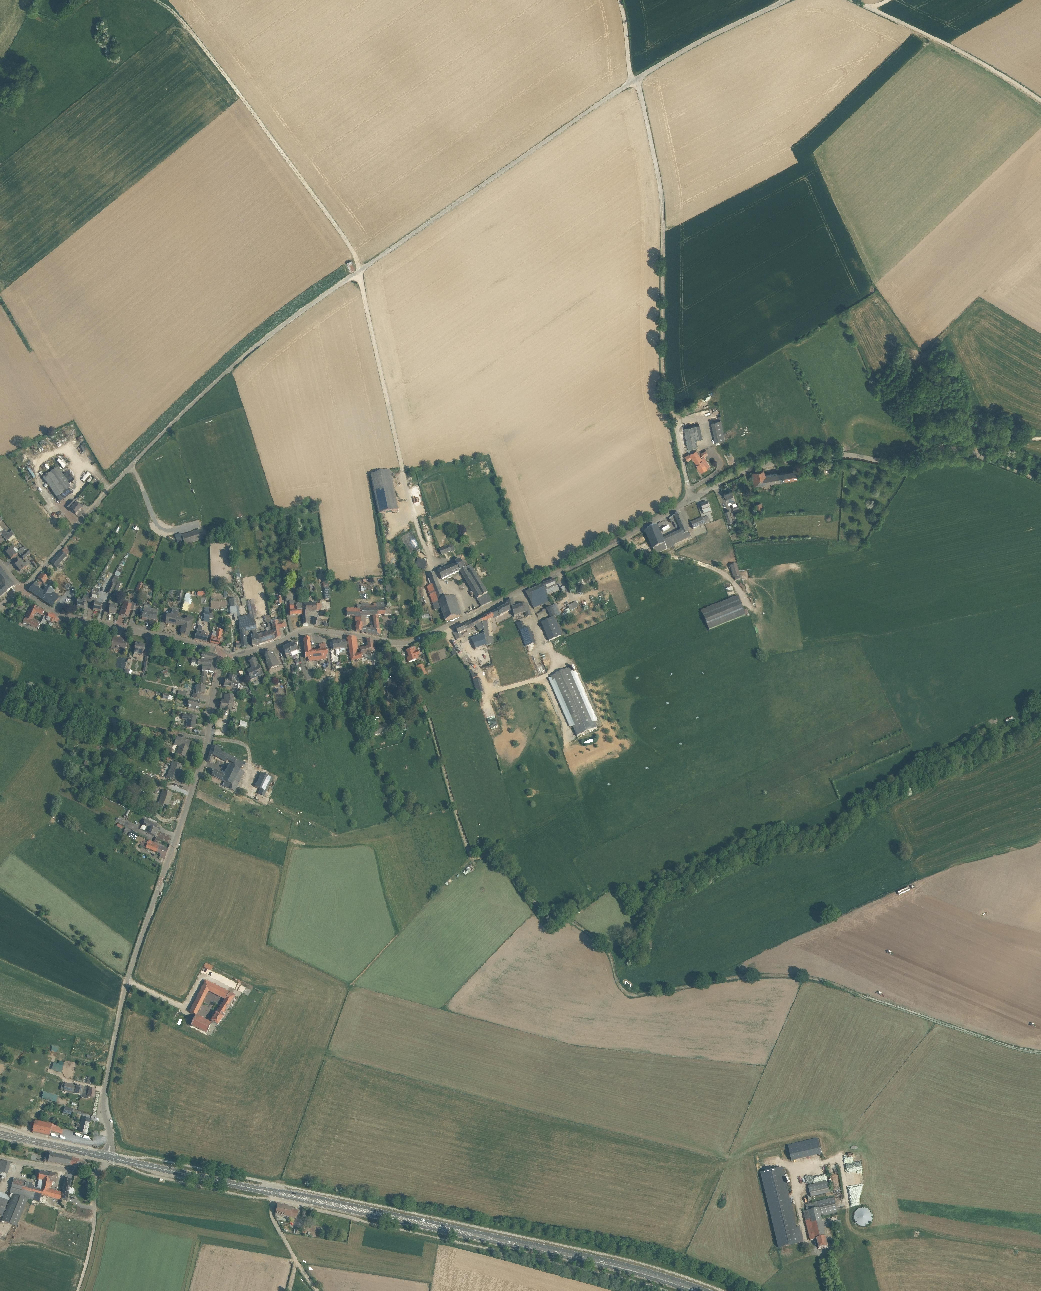
\includegraphics[width=0.3\linewidth]{Figures/full tile.png}
    \caption{Full AHN4 Sub-Tile}
    \label{figure1}
\end{figure}


\subsection{Step 2: Preparing the Dataset}
\noindent
The assigned tile has the following minimum and maximum x,y,z points(Table~\ref{table1}. The information was retrieved from using pdal.


\begin{minted}{bash}
pdal info 69BZ2_19.LAZ --summary
\end{minted}


\begin{table}[hbt!]
    \centering
    \renewcommand{\arraystretch}{1.5}
    \caption{X,Y,Z Boundaries of the Full Tile}
    \small
    \vspace{0.5\abovecaptionskip}
    \label{table1}
    \begin{tabular}{c|c|c}
        \hline
        \multirow{3}{*}{Max} & x & 189019.999\\   
                             & y & 315019.999\\  
                             & z & 206.948\\
         \hline
         \multirow{3}{*}{Min} & x & 187980\\  
                              & y & 313730\\  
                              & z & 132.642\\
        \hline
    \end{tabular}
\end{table}

\noindent Using the bounds \texttt{x:[188250,188750], y:[313992,314492]}, we cropped a 500m x 500m part from the tile as in Figure~\ref{figure2}.\\

\begin{figure}[hbt!]
    \centering
    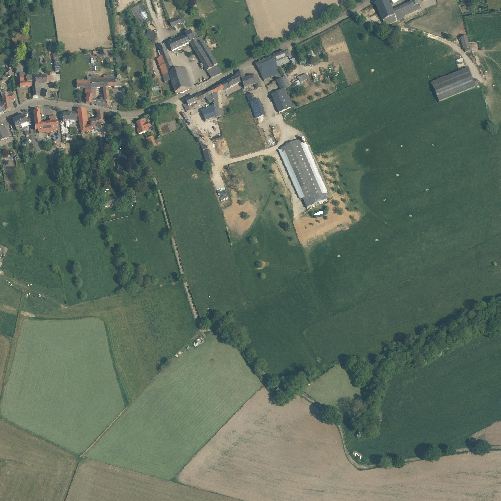
\includegraphics[width=0.4\linewidth]{Figures/cropped tile.png}
    \caption{Cropped 500x500}
    \label{figure2}
\end{figure}

\noindent A simple analysis on the percentages of the different classifications yielded the following result shown in Table~\ref{table2}.

\begin{table}[hbt!]
    \centering
    \renewcommand{\arraystretch}{1.5}
    \small
    \caption{Classification by Percentage}
    \vspace{0.5\abovecaptionskip}
    \begin{tabular}{c|cccc}
        \hline
         Classification  & 1 (unclassified) & 2 (ground)  & 6 (buildings)  & 9 (water)   \\
         \hline
         Percentage (\%) & 14.1316 & 82.5171  & 3.3481  & 0.0033 \\
         \hline
    \end{tabular}
    \label{table2}
\end{table}

\vspace{1cm}

\begin{figure}[hbt!]
    \centering
    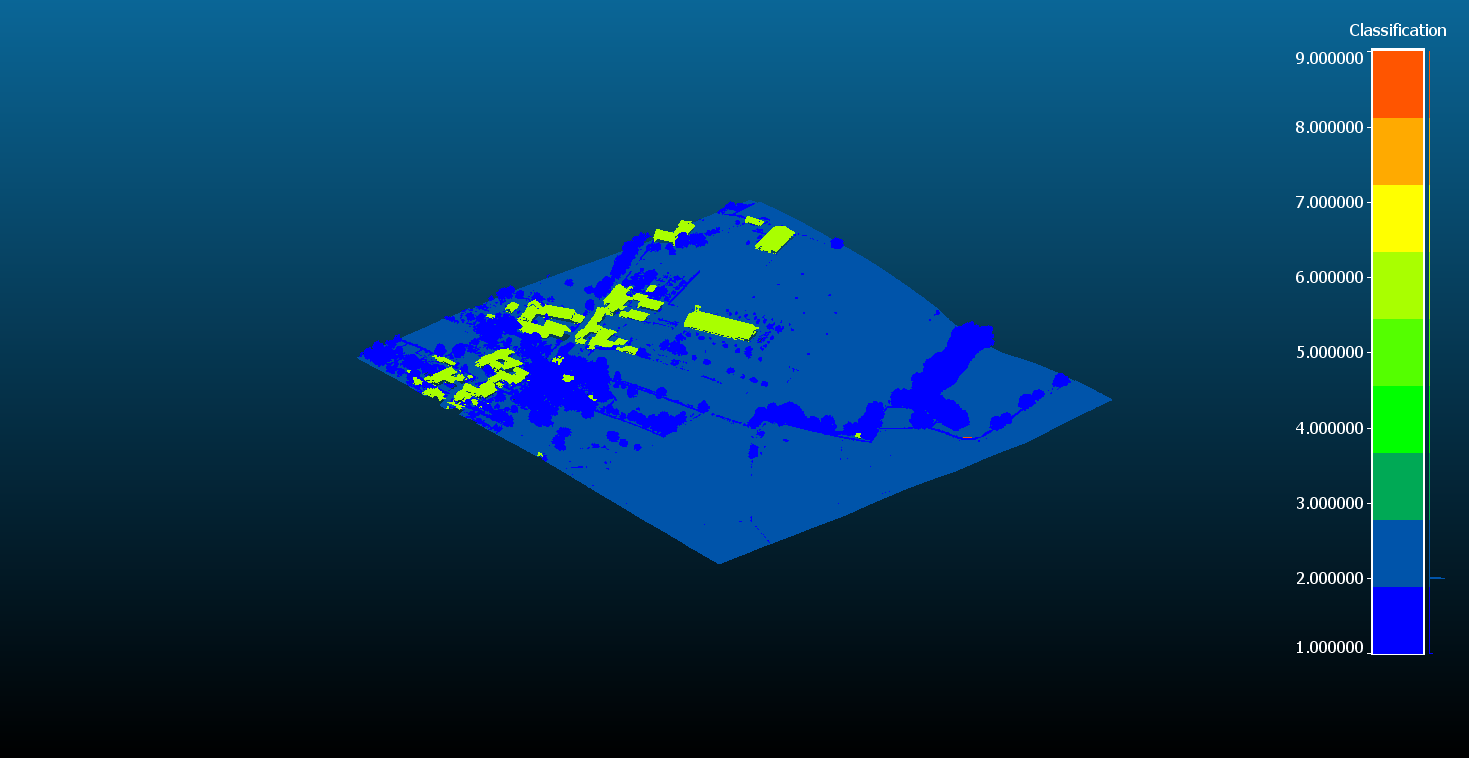
\includegraphics[width=0.6\linewidth]{Figures/classes_3d.png}
  \label{fig:3d_classes}
  \caption{Overview by Classifications in CloudCompare}
\end{figure}


\subsection{Step 3: GFTIN}\label{step3}

In the course of implementing the ground filtering algorithm for Digital Terrain Modeling, we encountered a number of challenges. The first major concern involved determining the optimal configuration for several key parameters: the distance threshold, the maximum angle for triangle slopes, and the size of the grid cells. Each of these parameters plays a crucial role in accurately distinguishing ground points from non-ground points, and finding the right balance was essential for the effectiveness of the algorithm.\\

\noindent The second challenge was managing the treatment of data at the boundaries of the study area. Edge effects can introduce significant distortions in terrain models, and thus require careful handling. Our approach needed to ensure that the algorithm remained robust at these boundary regions, without sacrificing the accuracy and integrity of the terrain model.


\subsubsection{Best Configuration of Key Parameters}
\textbf{Indicators}\\
\noindent In addressing the task of configuring key parameters for our ground filtering algorithm, we adopted a benchmark testing approach. Recognizing the plethora of available metrics to evaluate classification results, we selected accuracy and F1 score as our primary indicators. These metrics are frequently utilized in research focused on point cloud data classification due to their effectiveness in balancing the trade-off between precision and recall.\\

\noindent The formulas for these two metrics are as follows:\\

\noindent \textbf{Accuracy}: This is calculated as the ratio of correctly predicted observations (both true positives and true negatives) to the total observations in the dataset. It is a measure of overall correctness of the classification.

\[Accuracy = TP+TN/(TP+TN+FP+FN)\]

\noindent \textbf{F1 Score}: The F1 Score is the harmonic mean of precision and recall, providing a balance between the two. It is particularly useful in situations where there is an uneven class distribution.\\

\[F1Score = 2*(Precision*Recall)/(Precision+Recall)\]

\noindent Here, TP, TN, FP, and FN represent true positives, true negatives, false positives, and false negatives, respectively.\\

\noindent \textbf{Result}\\
Figure~\ref{fig4} illustrates the variation of both accuracy and F1 score in response to different values of the distance threshold. In this figure, the x-axis represents the distance threshold in meters, while the y-axis quantifies the accuracy and F1 score. This graphical representation is crucial for understanding how changes in the distance threshold impact the performance of our ground filtering algorithm. The dual metrics of accuracy and F1 score offer a comprehensive view of the algorithm's effectiveness, with accuracy reflecting the overall correctness of classifications and the F1 score providing insight into the balance between precision and recall for various threshold settings.\\

\noindent As depicted in Figure~\ref{fig4}, a notable observation is that both accuracy and F1 score reach their peak performance at a 5-meter distance threshold. This finding highlights the optimal setting for the distance threshold in our algorithm, underlining its significance in achieving the most effective balance between accuracy and precision-recall trade-off in point cloud data classification.\\

\begin{figure}[hbt!]
    \centering
    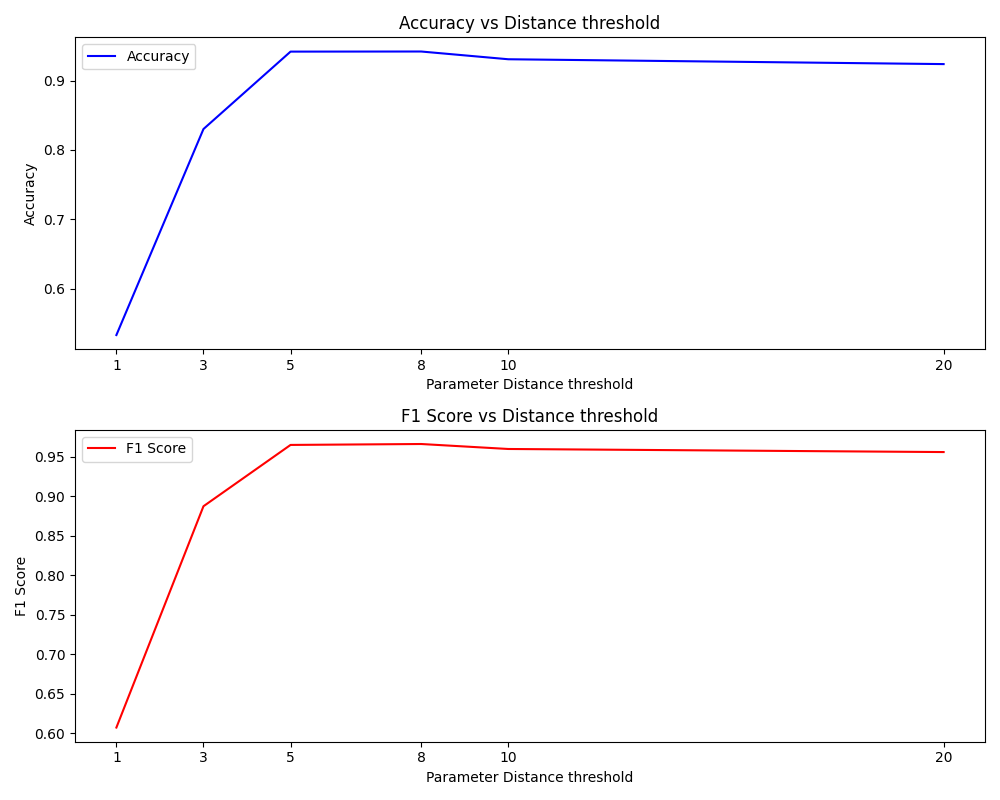
\includegraphics[width=0.6\linewidth]{Figures/benchmark_Distance Threshold.png}
    \caption{Benchmark: Distance Threshold}
    \label{fig4}
\end{figure}

\noindent On the other hand, Figure~\ref{fig5} focuses on the influence of varying the maximum angle in degrees between the triangle planes and perpendicular lines extending from points. This figure is instrumental in illustrating how these angular adjustments affect the chosen indicators of performance. As Figure~\ref{fig5} indicates, the most effective angle for our algorithm appears to be around 30 degrees. This specific angle demonstrates the optimal balance in our ground filtering process, as reflected in the performance metrics.\\

\begin{figure}[hbt!]
    \centering
    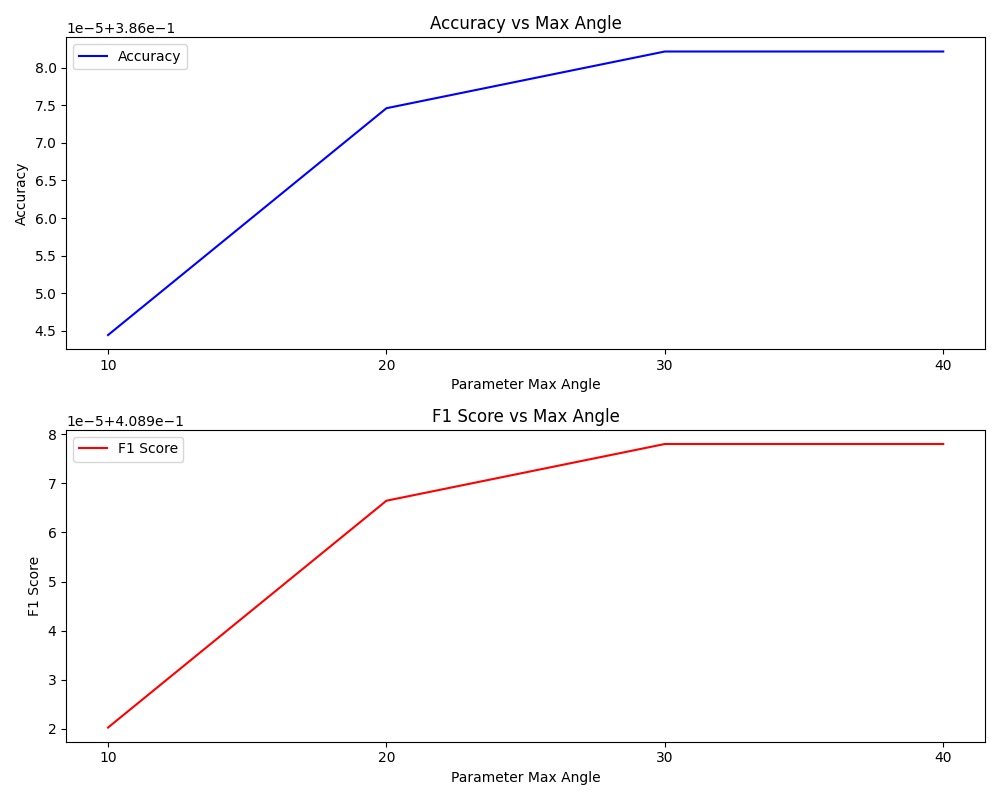
\includegraphics[width=0.6\linewidth]{Figures/benchmark_Max Angle.png}
    \caption{Benchmark: Max Angle}
    \label{fig5}
\end{figure}


\noindent Meanwhile, Figure~\ref{fig6} shifts the focus to the impact of cell size on our algorithm's performance. The cell size is a critical parameter in the process of extracting the lowest points for triangulation. As illustrated in Figure~\ref{fig6}, a cell size of 90 meters yields the best performance in terms of both accuracy and F1 score. This insight is significant as it guides the optimal setting for cell size in our algorithm, ensuring the most effective triangulation process for our digital terrain modeling.\\


\begin{figure}[hbt!]
    \centering
    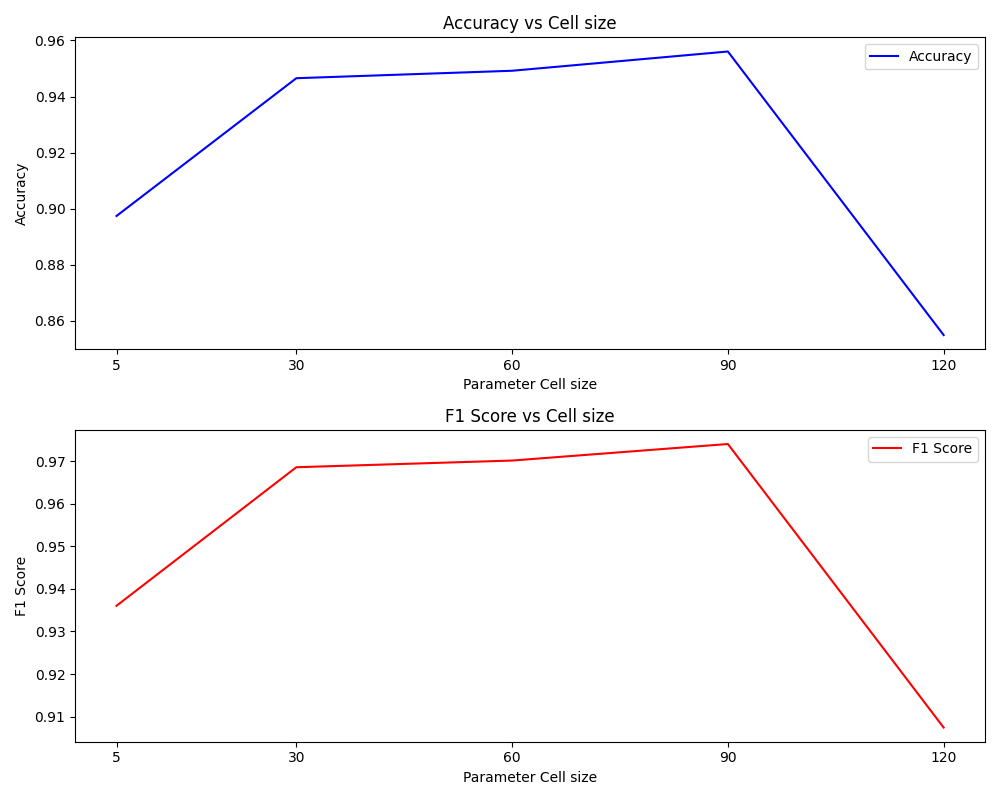
\includegraphics[width=0.6\linewidth]{Figures/benchmark_Cell size.png}
    \caption{Benchmark: Cell Size}
    \label{fig6}
\end{figure}

\noindent This benchmark analysis has conclusively identified the optimal configurations for the three key parameters in our ground filtering algorithm. Specifically, the ideal settings are determined to be a distance threshold of 5 meters, a maximum angle of 30 degrees, and a cell size of 90 meters. These configurations represent the most effective combination for achieving superior accuracy and F1 score in our digital terrain modeling process.

\subsubsection{Handling Data at the Boundaries}
The next challenge we faced was effectively handling the data at the boundaries of our study area. In our algorithm, a triangular network is constructed using the lowest point of each grid cell. However, we encountered an issue where numerous points fell outside the convex hull of the triangulation network. This scenario posed a significant problem because points not underlain by any triangle in the network couldn't be definitively classified as ground or non-ground.\\

\noindent To address this issue, we implemented a solution involving the addition of a buffered area around the study region. This buffer ensured that the triangulation network extended beyond the actual boundaries of our study area, thereby encompassing all points within its scope. As a result of this approach, the problem of unclassified points at the edges was effectively resolved. The triangulation network now adequately covers the entire study area, allowing for a complete and accurate ground classification.

\subsubsection{Evaluation of Our Program}

In the final stage of step 3, we conducted an evaluation of our program's performance. To rigorously evaluate the performance of our program, we employed two distinct approaches. The first approach involved a comparative analysis with the AHN DTM. By overlaying our program's DTM output with the AHN DTM, we were able to conduct a detailed spatial comparison. This allowed us to pinpoint specific areas where our model achieved high accuracy, as well as identify regions where accuracy was comparatively lower. This comparative method is particularly valuable as it provides a visual and spatial understanding of our model's performance against a well-established ground truth.\\

\noindent The second approach was centered around the calculation of statistical indicators. This involved deriving quantitative metrics such as accuracy, precision, recall, and F1 score, among others, from our model's outputs. These indicators offer a comprehensive view of the model's performance by quantifying its effectiveness in terms of error rates, the balance between sensitivity and specificity, and overall classification correctness. This statistical analysis complements the spatial comparison by providing a numerical basis for evaluating and benchmarking our model's performance.\\

\noindent \textbf{Comparison with AHN4's DTM}\\
Figure~\ref{fig7} introduces our study area, providing a baseline for comparison. Figure~\ref{fig8} and Figure~\ref{fig9} are particularly pivotal, as they display DTM of the same area. Figure~\ref{fig8} presents the DTM provided by the AHN, which serves as our ground truth, while Figure~\ref{fig9} showcases the DTM generated by our program. A key observation is the conspicuous similarity between our program's output and the AHN DTM, affirming the effectiveness of our methodology. Notably, the AHN DTM exhibits 'no data' values in regions where buildings are located.\\

\begin{figure}[H]
    \centering
    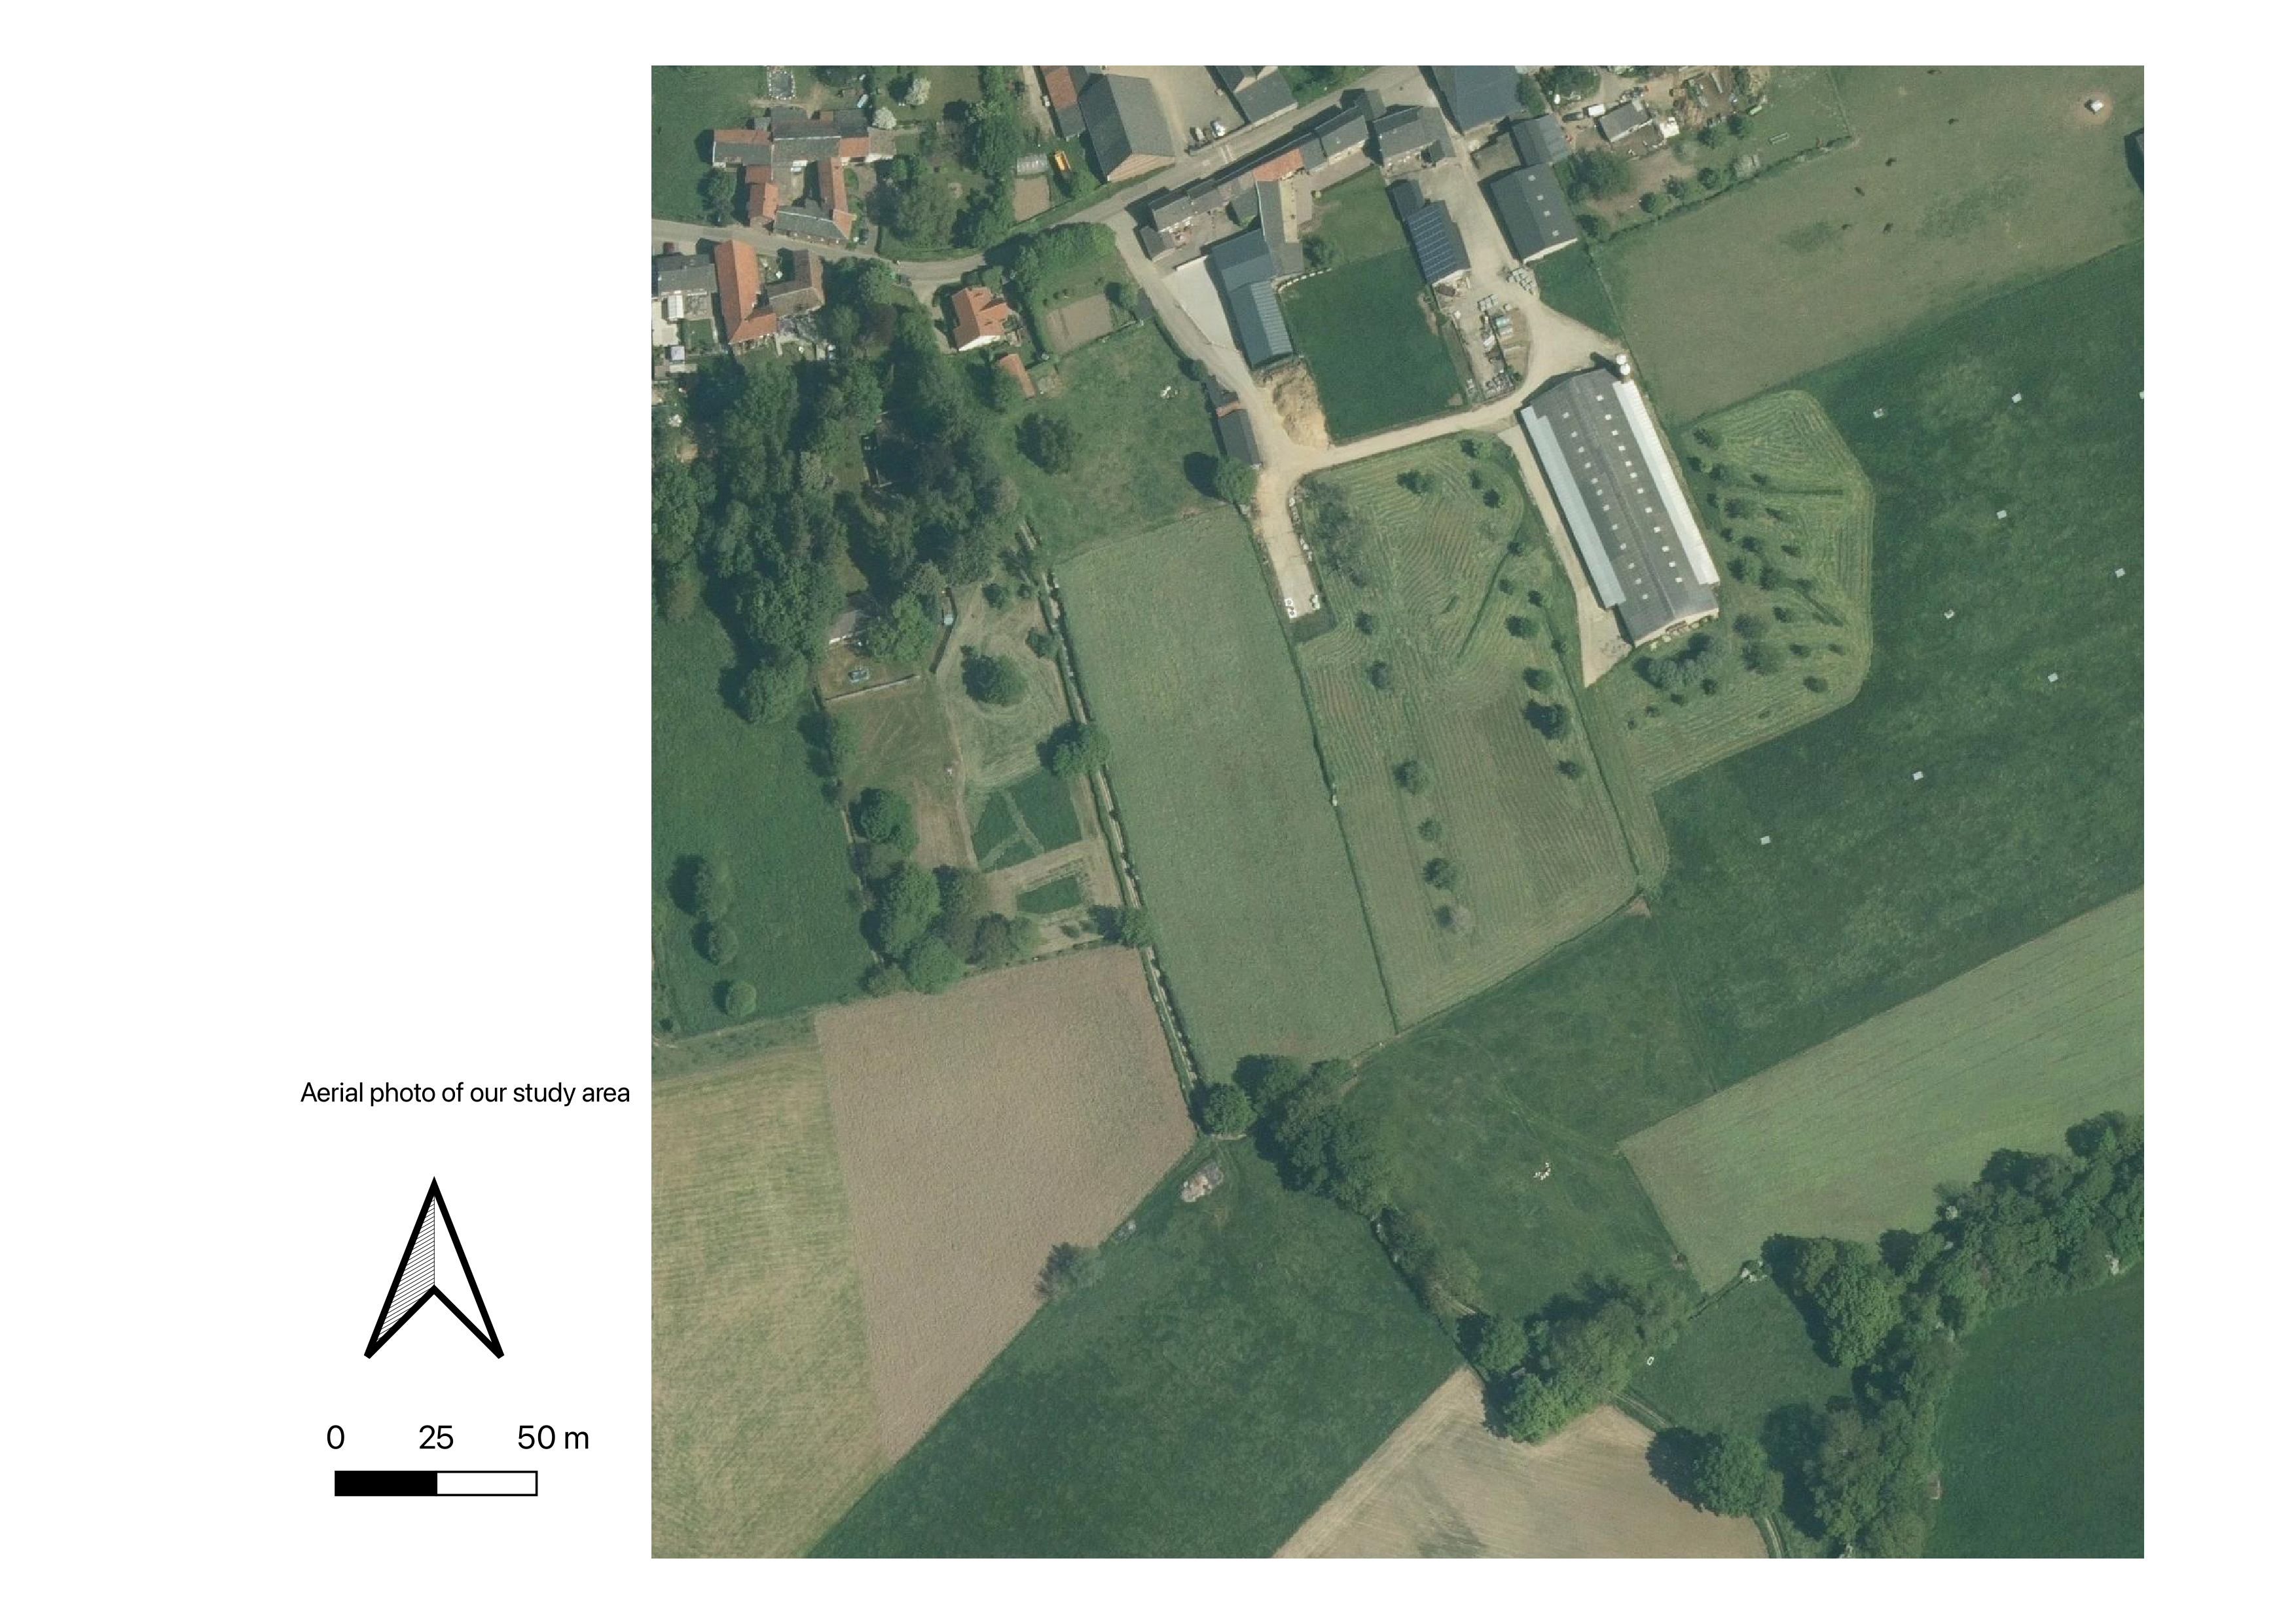
\includegraphics[width=0.5\linewidth]{Figures/fg7.png}
    \caption{Aerial Photo}
    \label{fig7}
\end{figure}


\begin{figure}[H]
    \centering
    \subfloat[ANH4 DTM]{%
        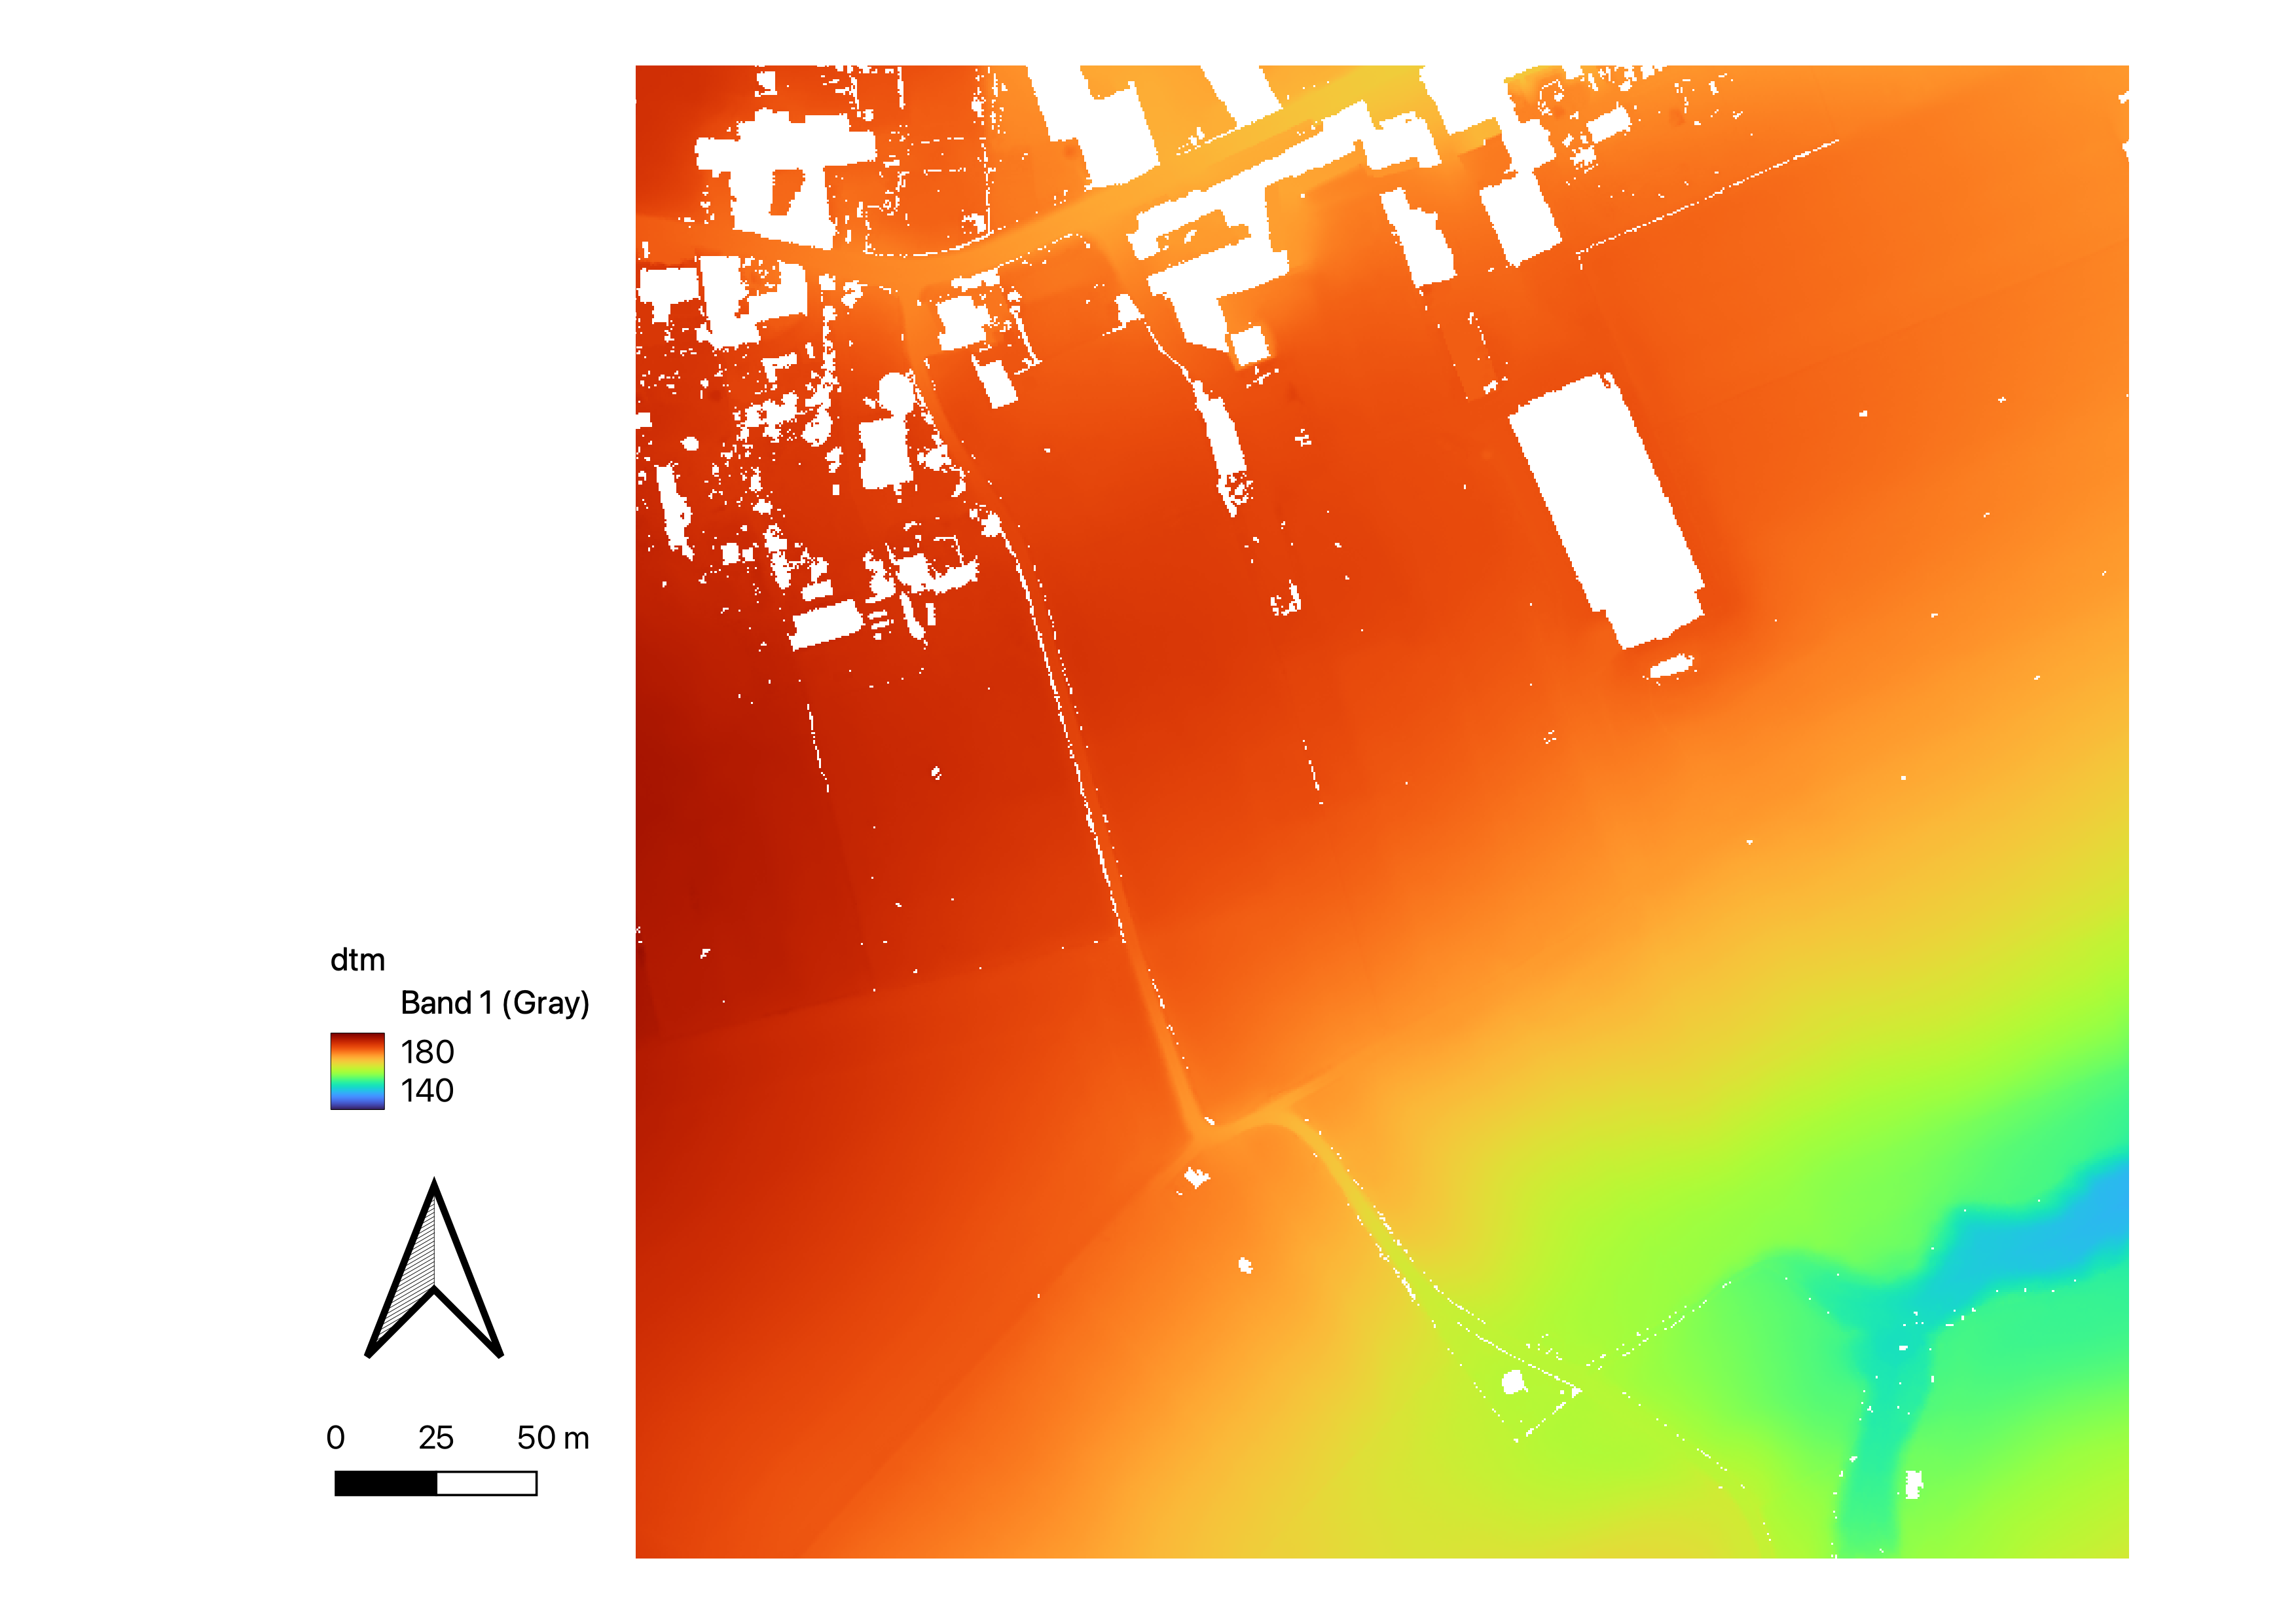
\includegraphics[width=0.45\linewidth]{Figures/fig8.png}
        \label{fig8}
    }
    \hspace{0.5cm}
    \subfloat[Our DTM]{%
        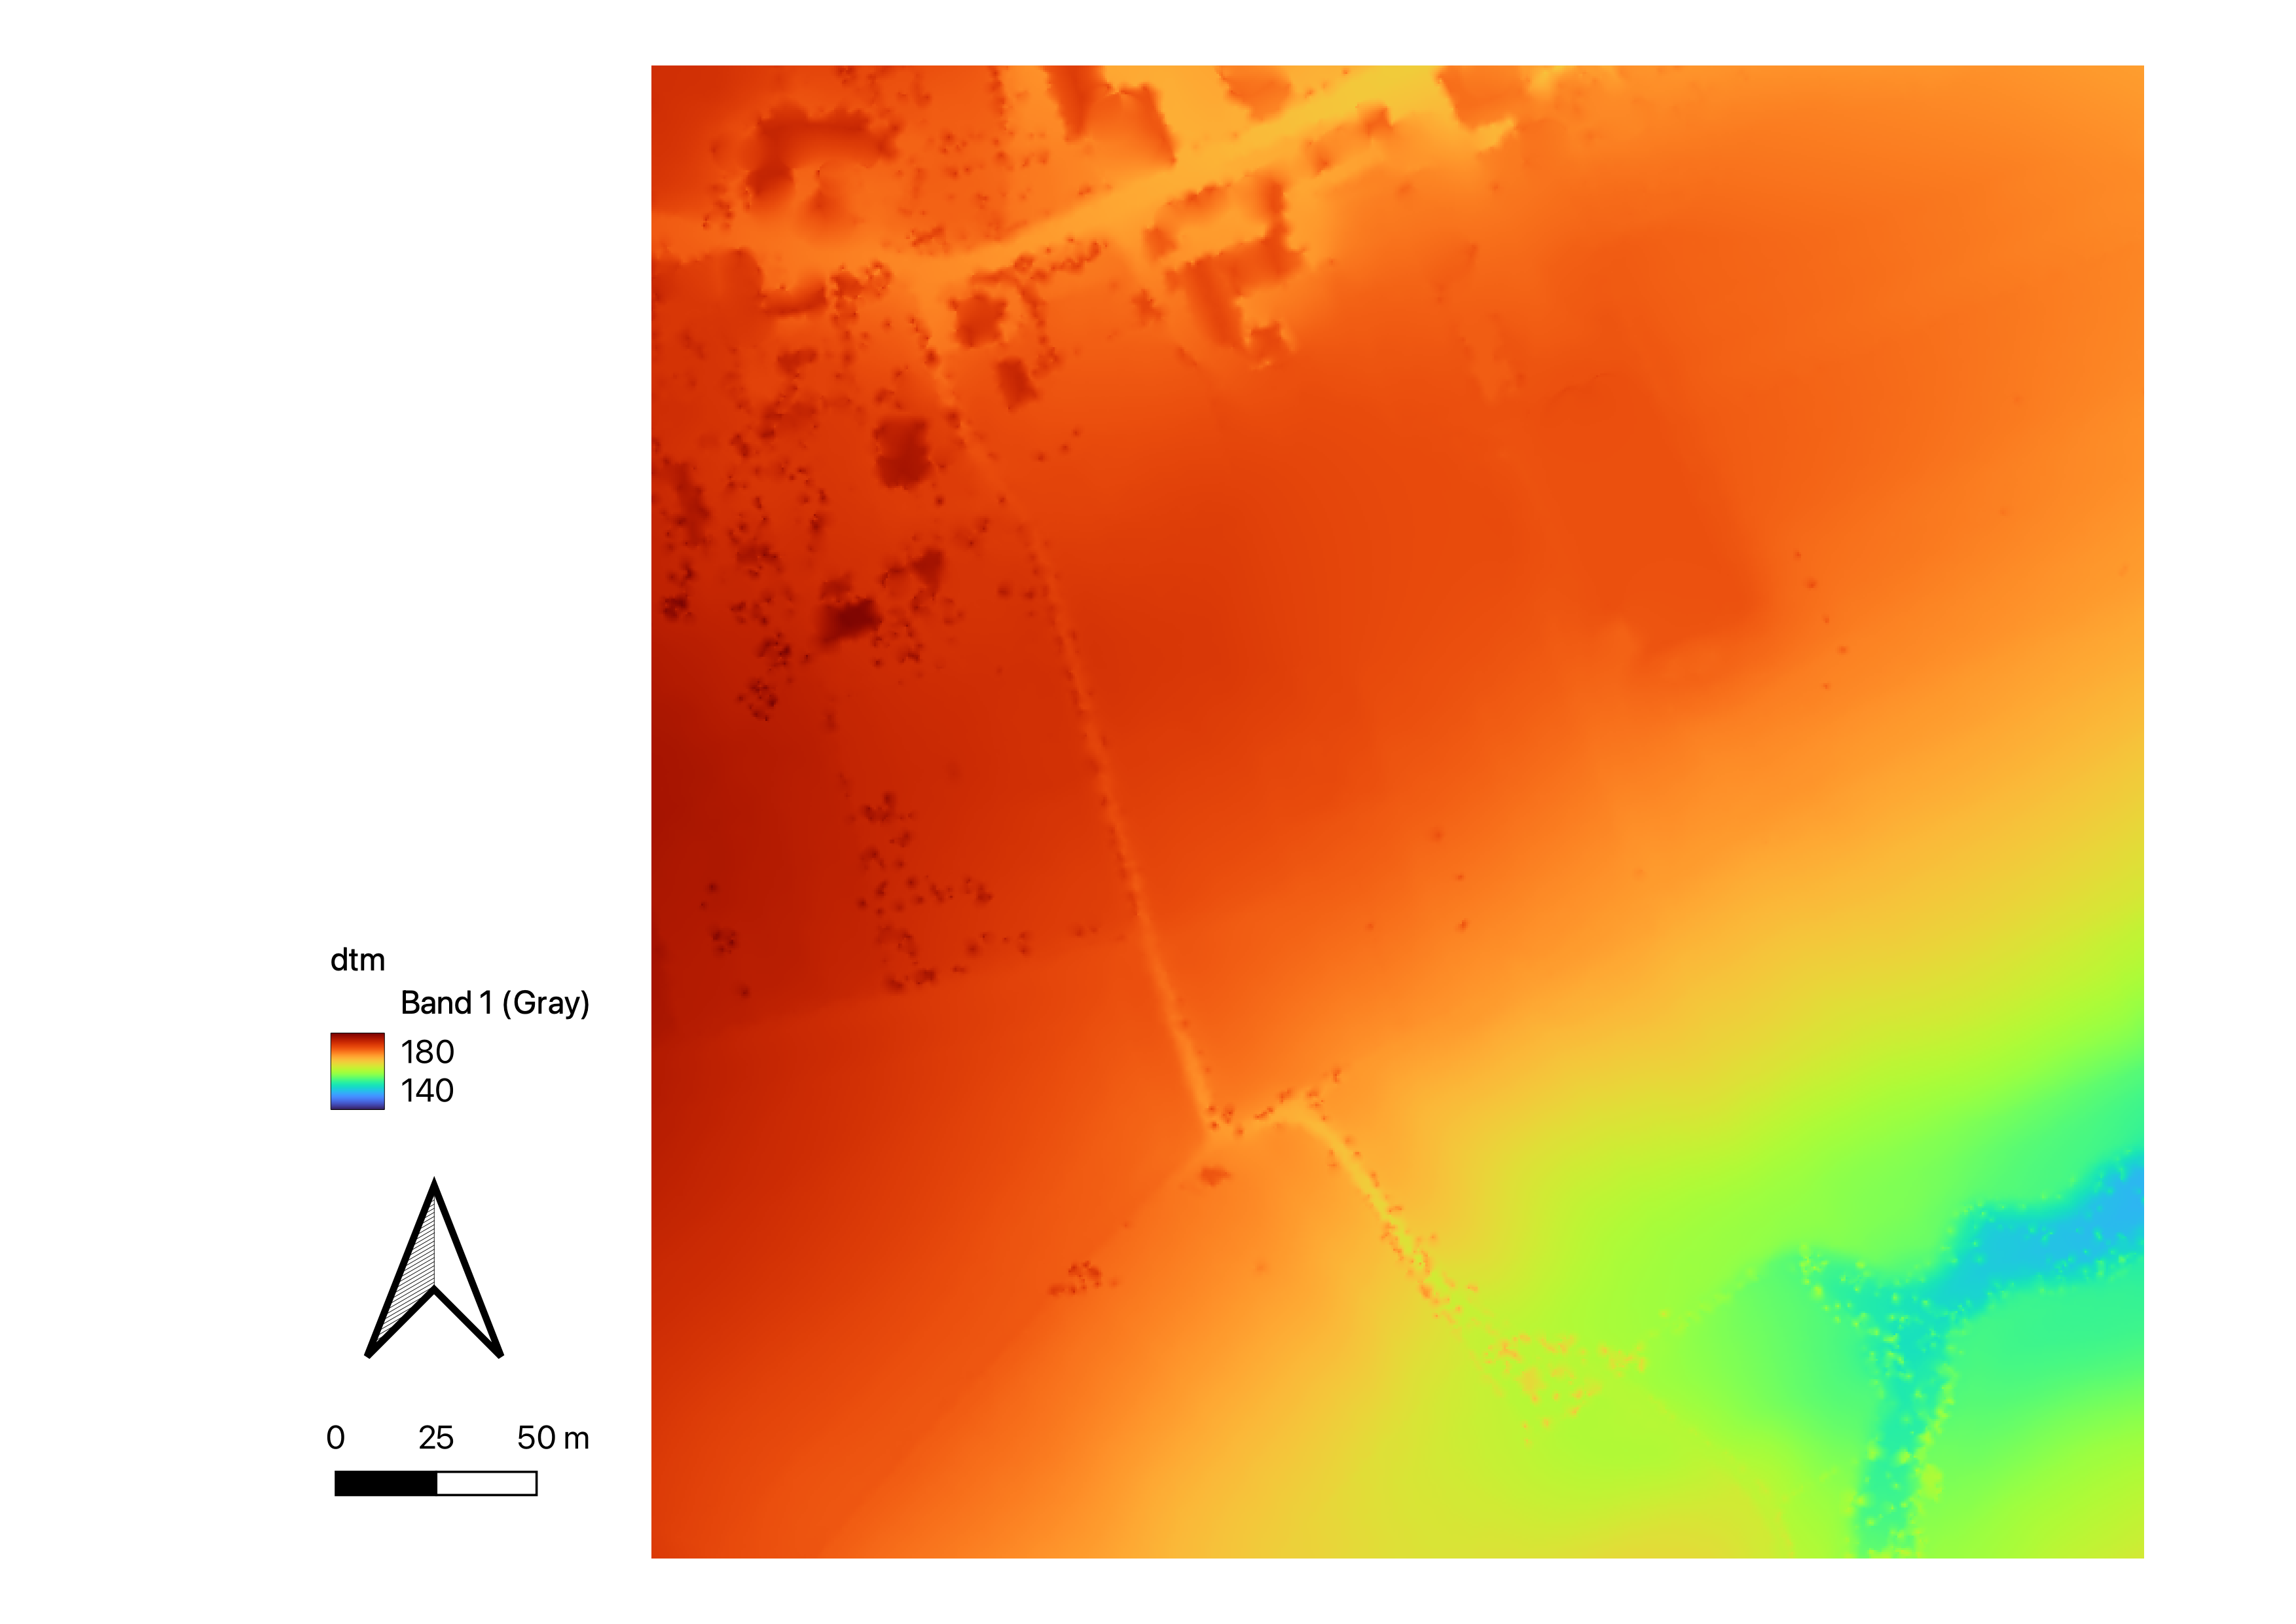
\includegraphics[width=0.45\linewidth]{Figures/fig9.png}
        \label{fig9}
    }
    \caption{Comparison of DTMs}
    \label{fig:comparison}
\end{figure}

\noindent Figure~\ref{fig10} is instrumental in detailing the height differences between the AHN DTM and our program's DTM. In this figure, all values are represented as absolute values to account for both positive and negative discrepancies. This comparison allows for a nuanced understanding of the variances in elevation data between the two models.\\

\noindent Finally, Figures~\ref{fig11} and Figure~\ref{fig12} are dedicated to illustrating areas of varying accuracy within our program's DTM. Figure Figure~\ref{fig11} highlights regions where our model demonstrates high accuracy, while Figure~\ref{fig12} identifies areas where the accuracy is relatively lower. This granular analysis is crucial in understanding the spatial distribution of our model's performance across the study area.\\

\begin{figure}[H]
    \centering
    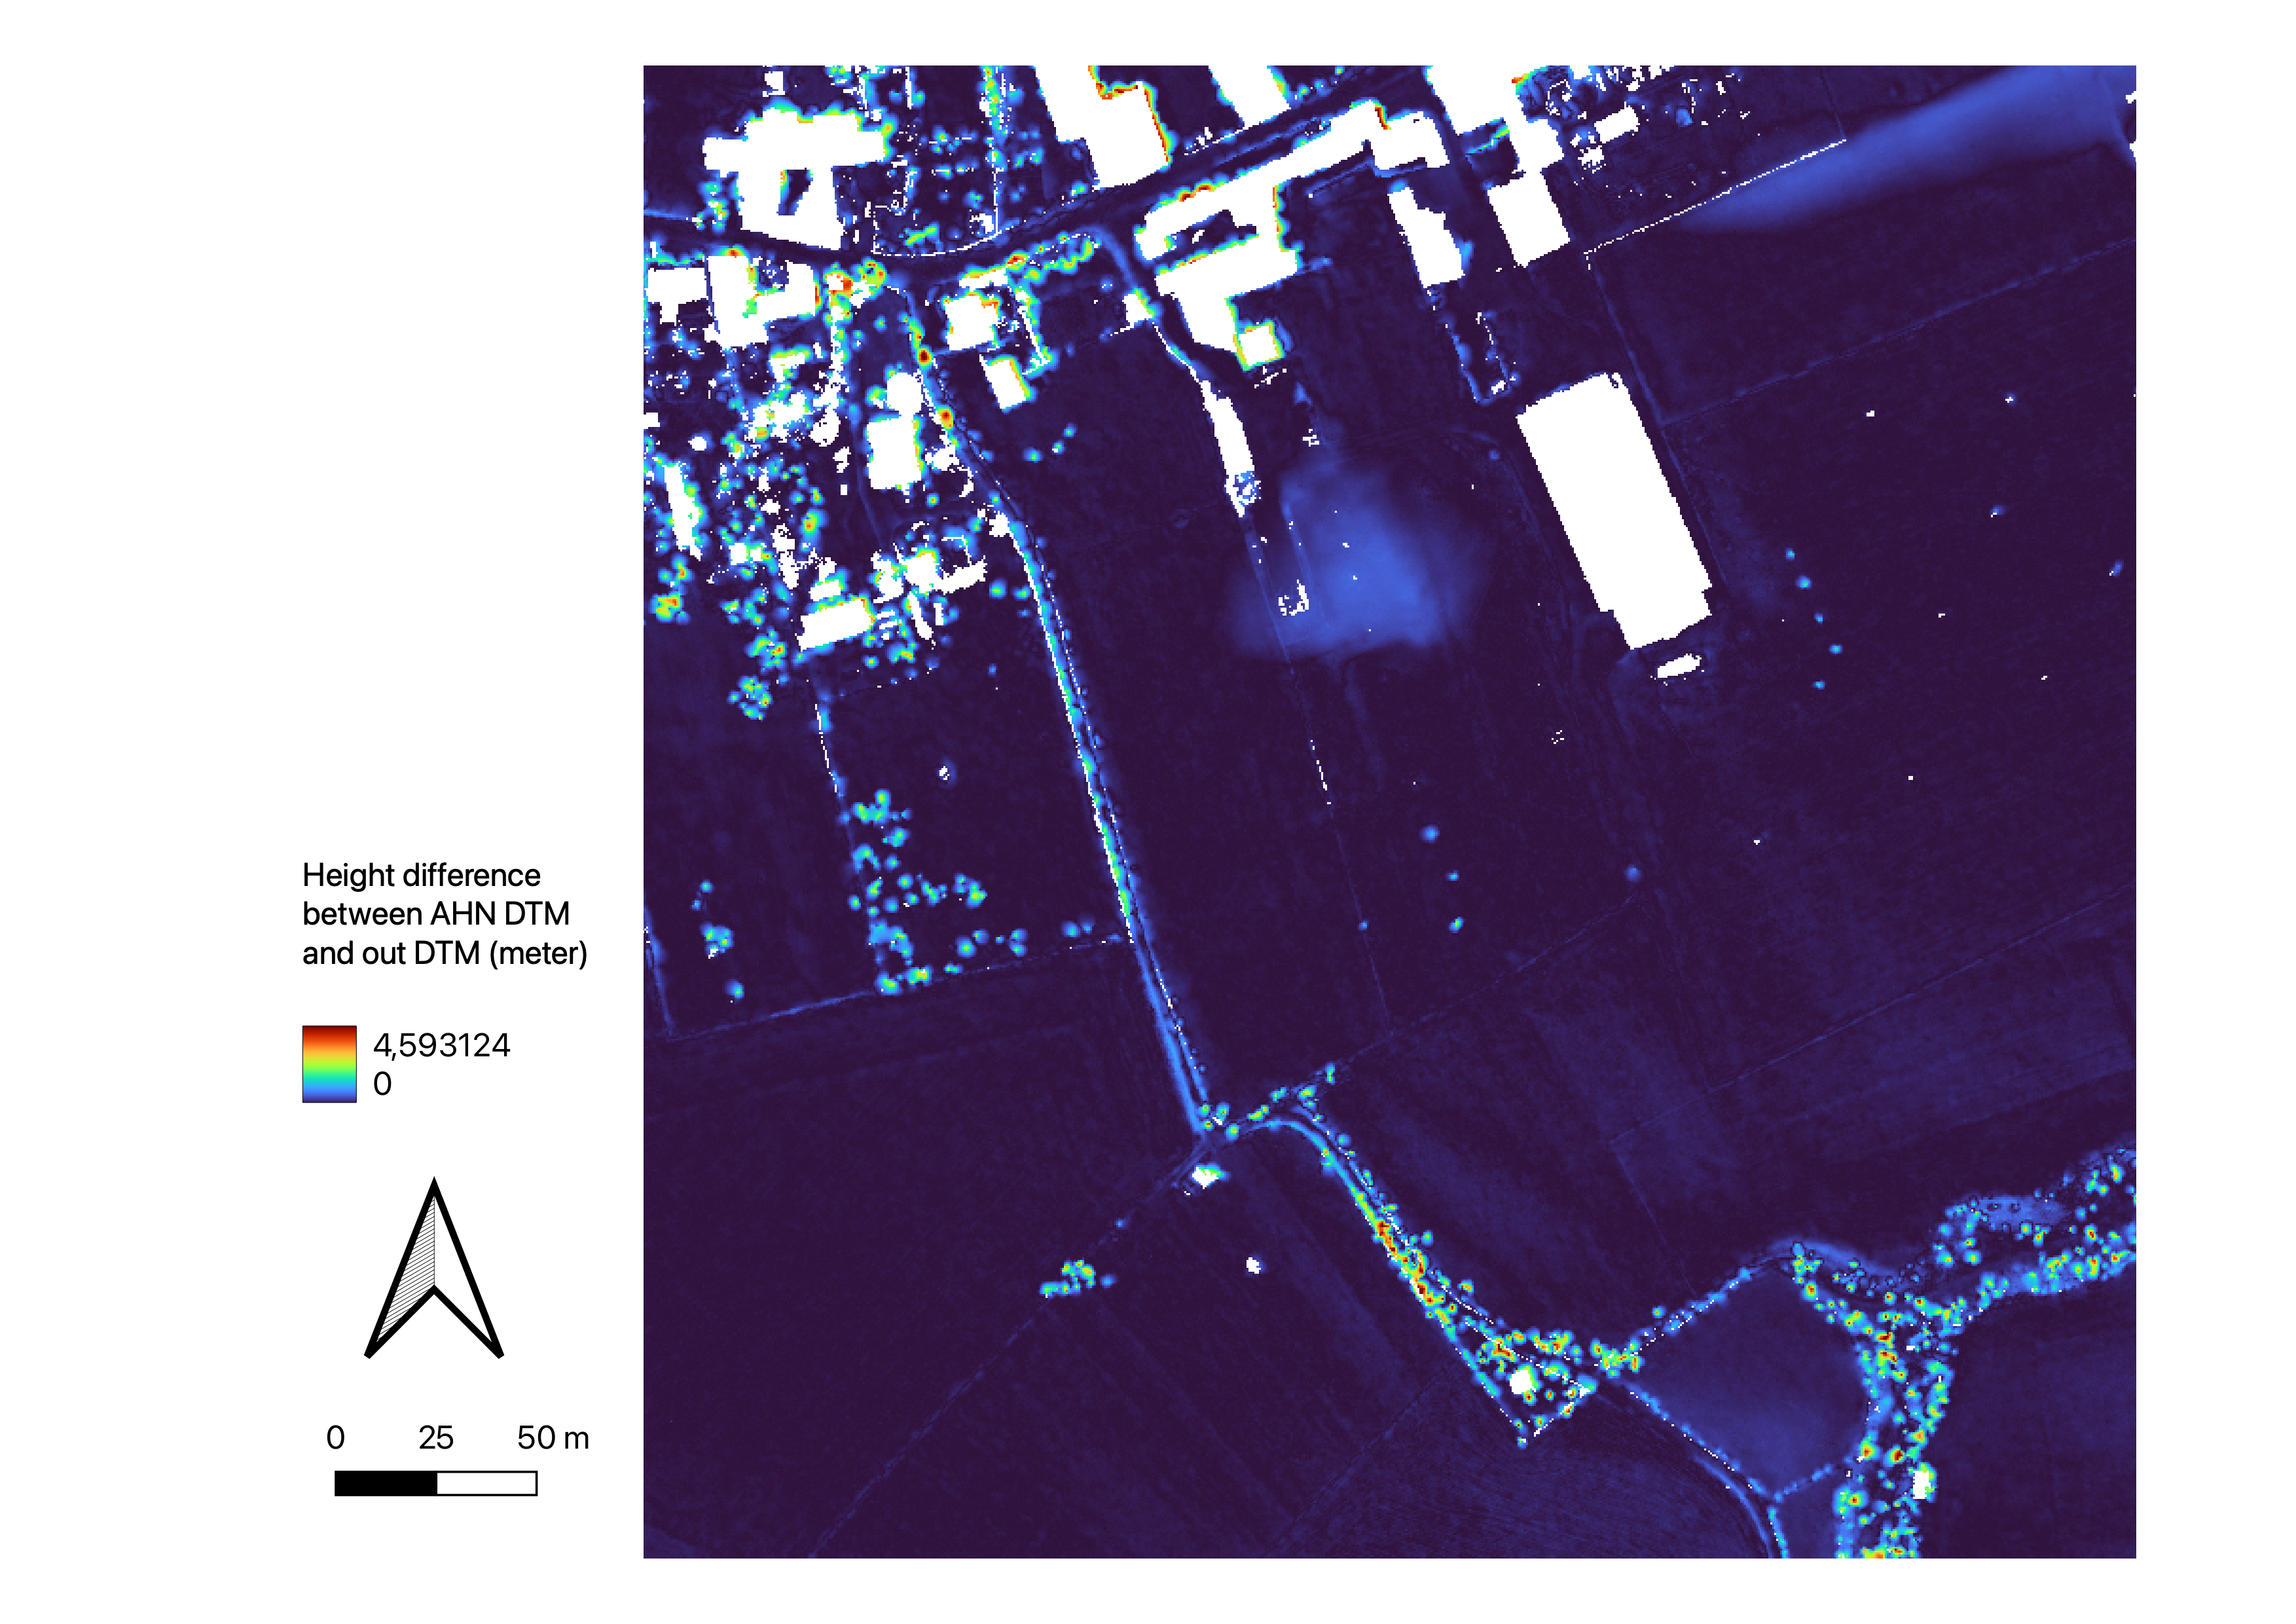
\includegraphics[width=0.7\linewidth]{Figures/fig10.png}
    \caption{Height Difference with AHN}
    \label{fig10}
\end{figure}

\noindent Figure~\ref{fig11} provides compelling evidence of the high performance of our program in areas dominated by grass and soil. In these regions, the error margin is impressively small, typically ranging from 0 to 0.5 meters. This accuracy underscores our program's effectiveness in handling terrain with relatively uniform and low-lying features.\\

\noindent Conversely, Figure~\ref{fig12} highlights the challenges our program faces in accurately modeling areas with tall objects. Here, the accuracy is notably lower, suggesting a need for further refinement in our approach for these types of landscapes. To address this issue, adjusting the three key parameters—distance threshold, maximum angle, and cell size—is crucial. However, this tuning presents a trade-off: reducing the distance threshold and maximum angle may indeed enhance the exclusion of high tall objects, thereby improving accuracy in these specific areas. Yet, such adjustments could simultaneously lead to an increase in the number of false positives, indicating a lower likelihood of incorrectly classifying ground points as non-ground.\\

\noindent This observation points to a fundamental challenge in digital terrain modeling: finding the optimal balance between accurately capturing complex features like tall objects and maintaining overall classification accuracy. Our future efforts will focus on fine-tuning these parameters to achieve a more balanced and accurate representation across varied terrain types.\\




\begin{figure}[H]
    \centering
    \subfloat[Less Difference Around Grass]{%
        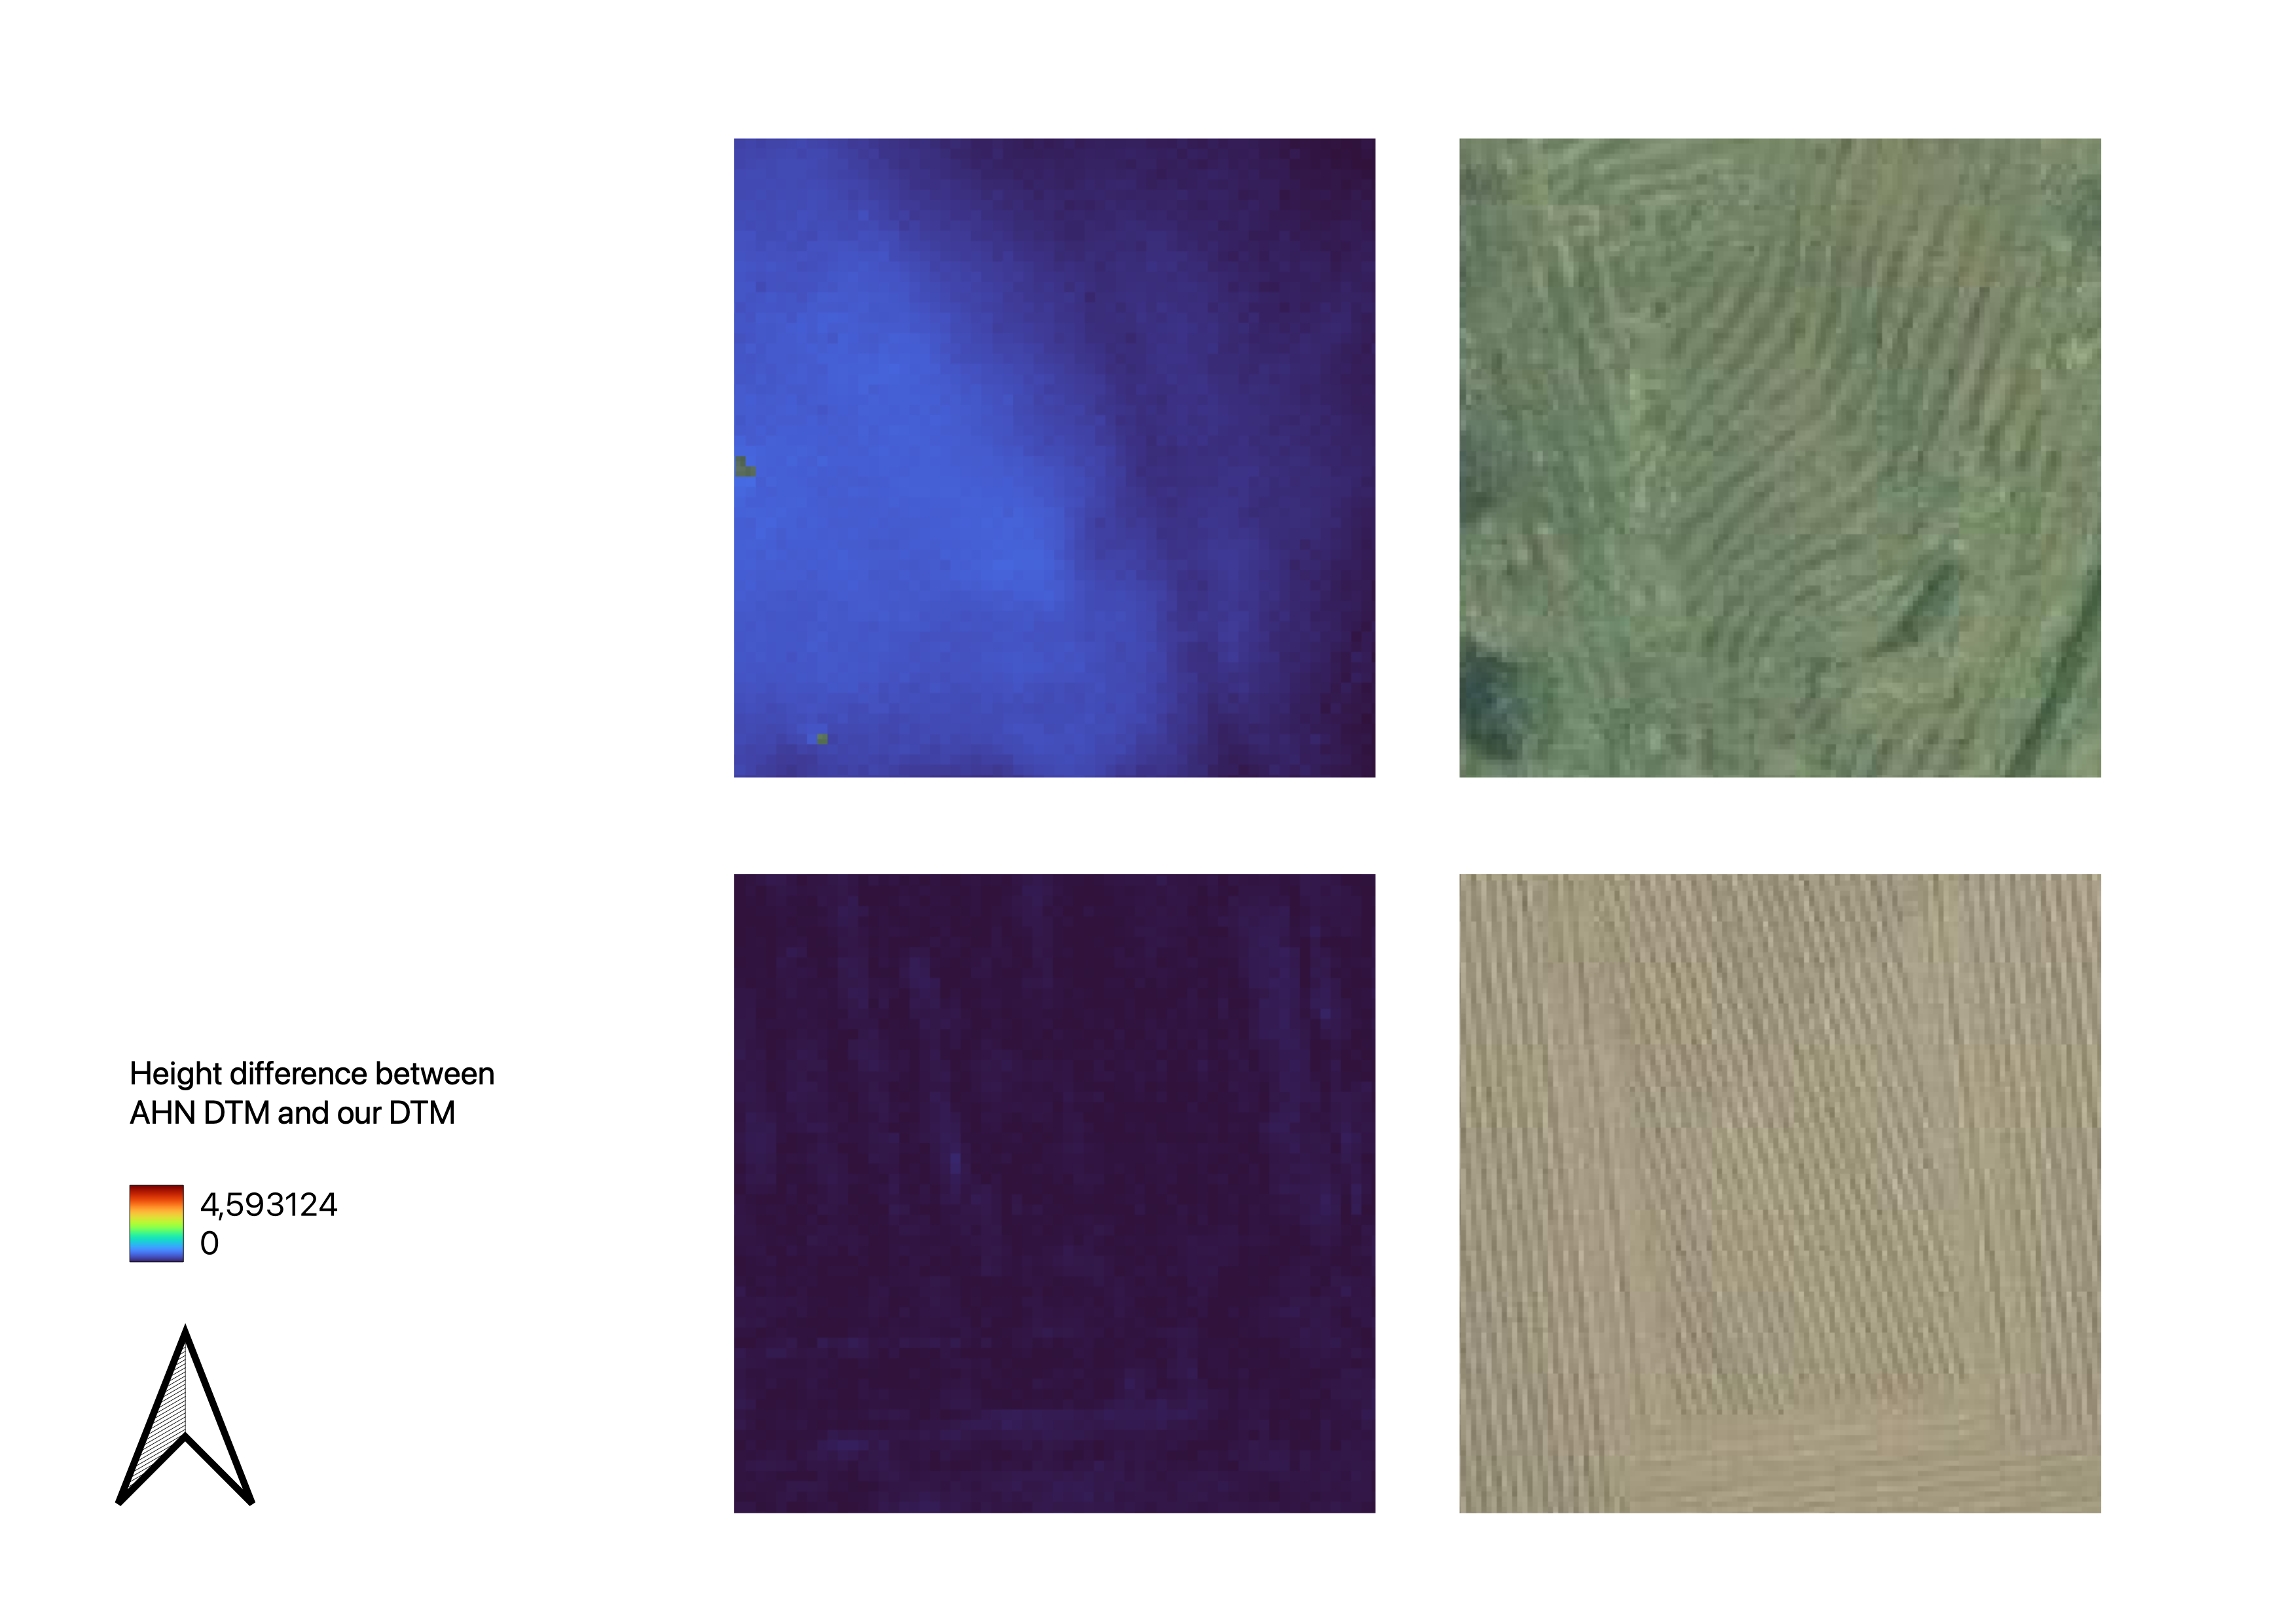
\includegraphics[width=0.45\linewidth]{Figures/fig11.png}
        \label{fig11}
    }
    \hspace{0.5cm}
    \subfloat[More Difference Around Higher Objects]{%
        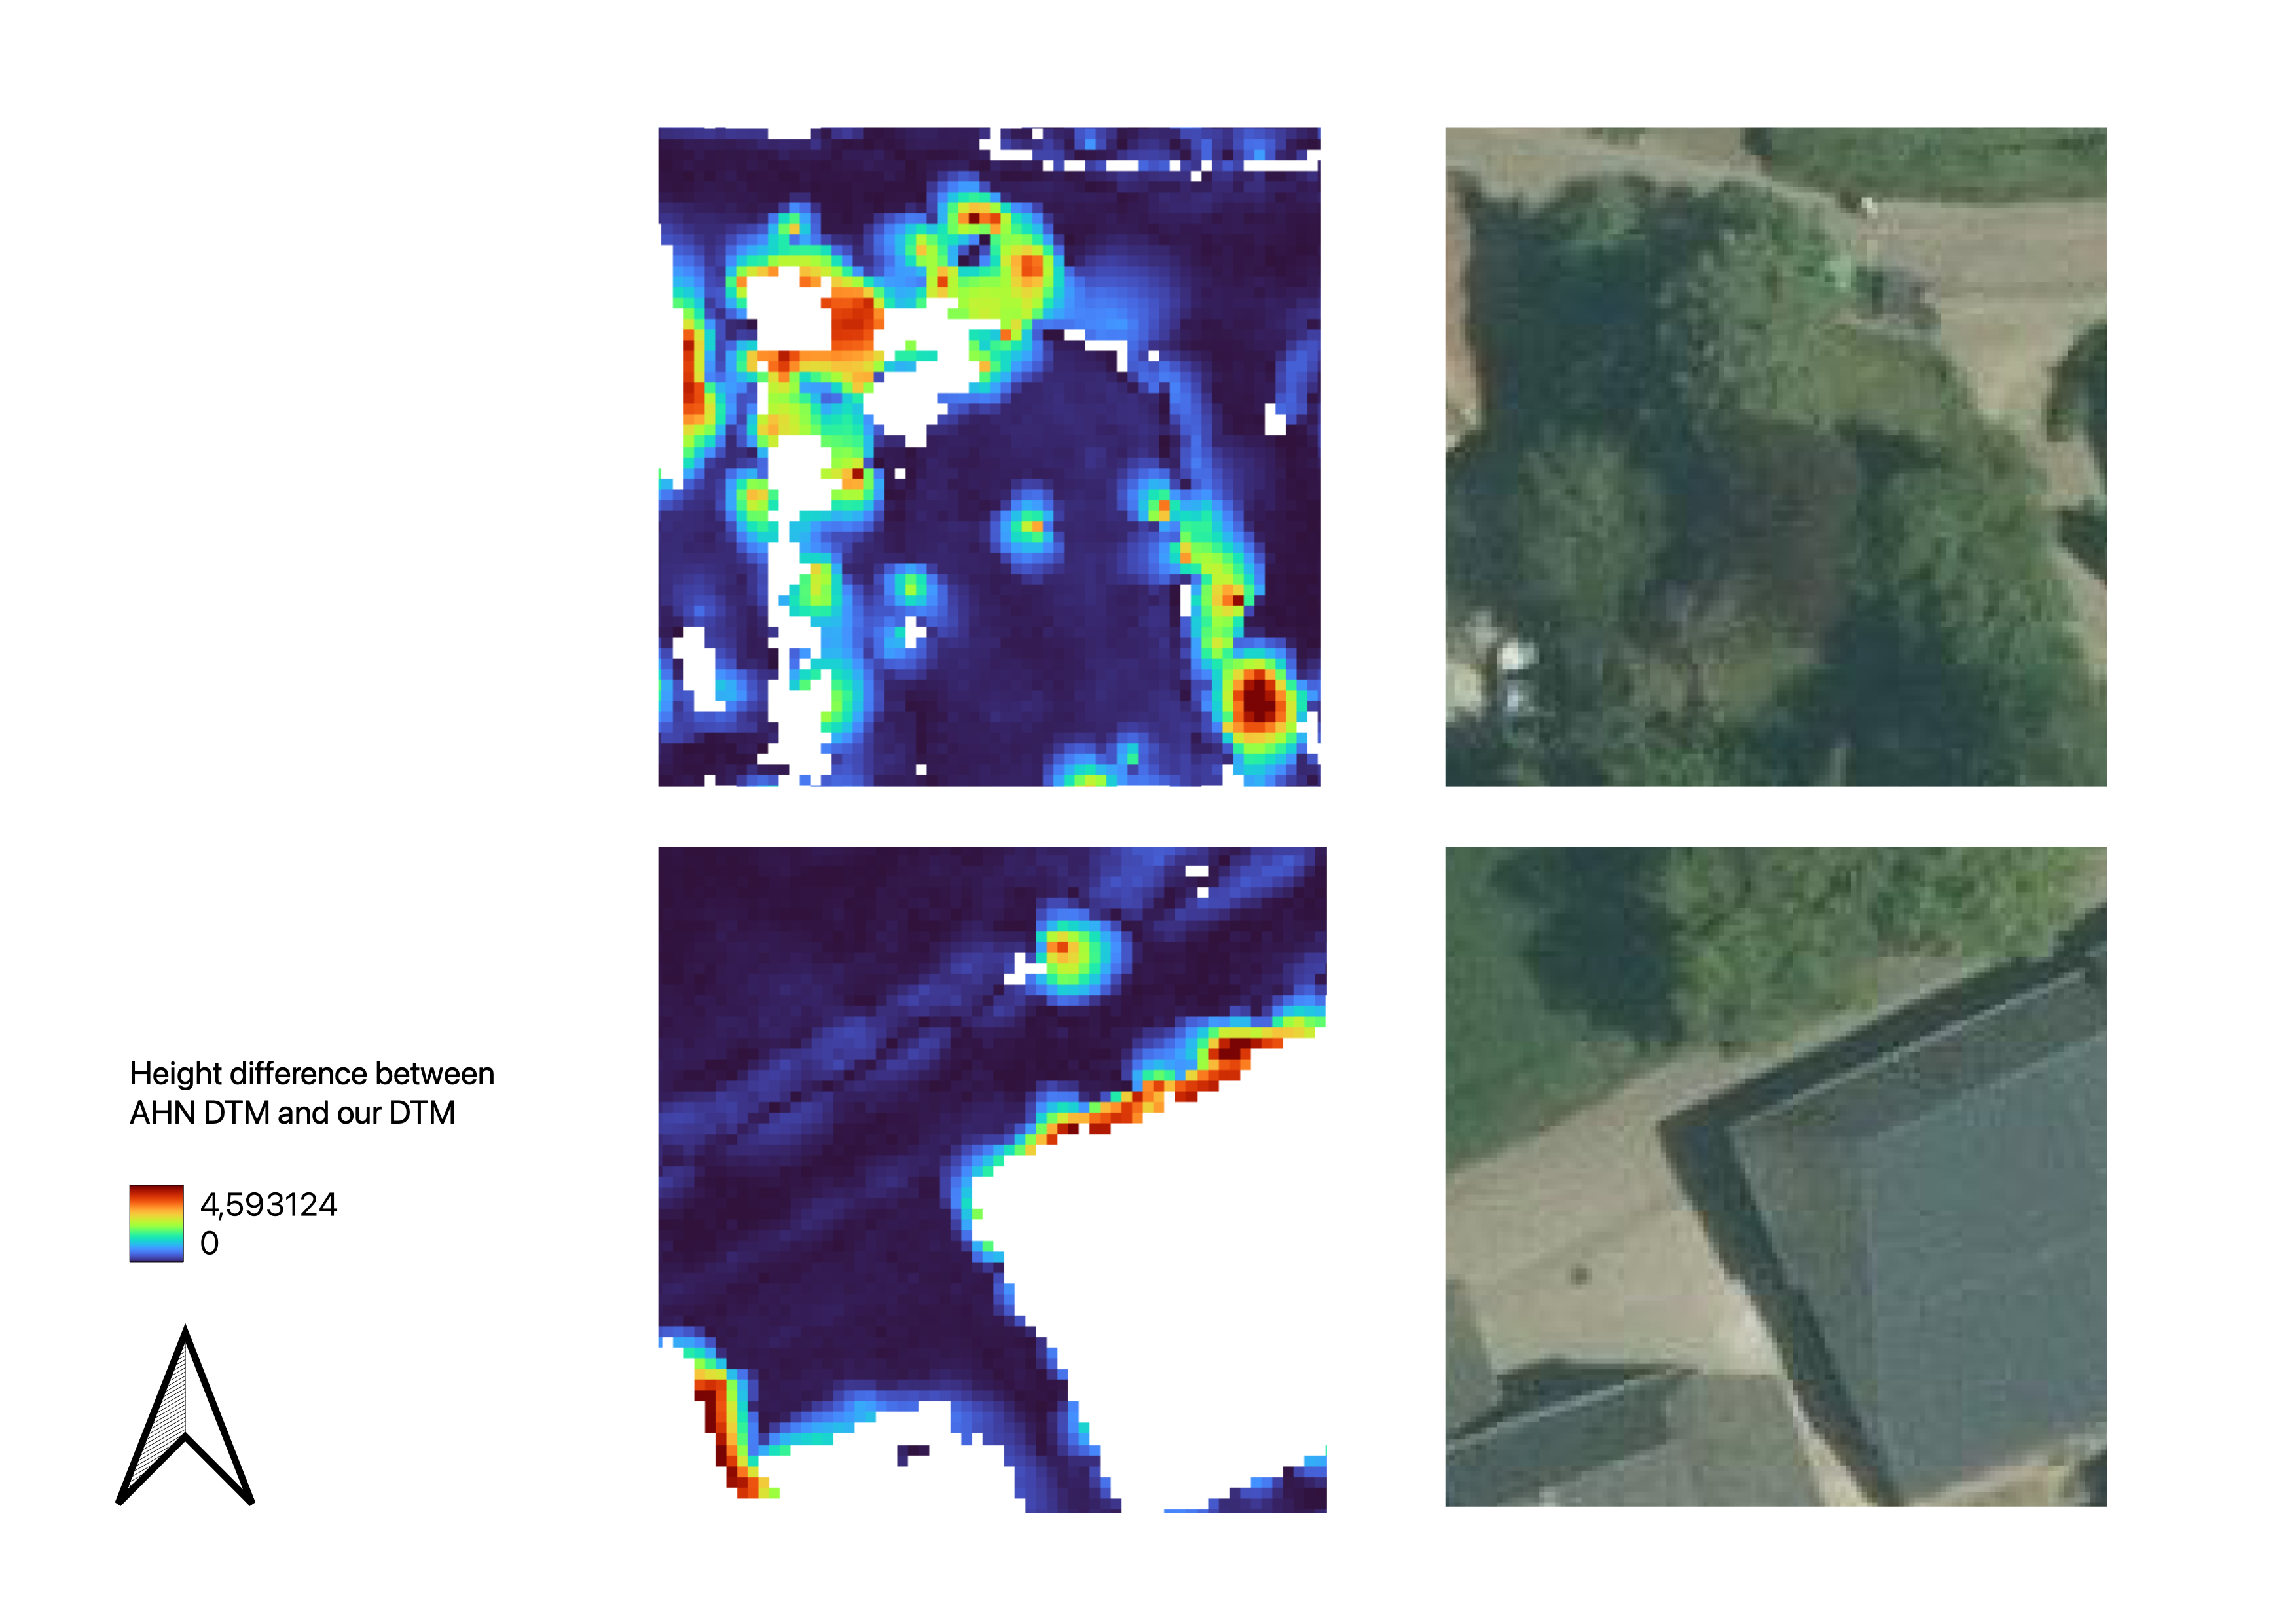
\includegraphics[width=0.45\linewidth]{Figures/fig12.png}
        \label{fig12}
    }
    \caption{Comparison of Results}
    \label{fig:comparison}
\end{figure}


\noindent \textbf{Statistical Indicators}\\
The Table~\ref{table3} presented elucidates the results achieved using the optimal configuration of parameters as determined by our benchmark analysis. Upon processing a substantial dataset of 3,313,199 points, the algorithm demonstrated impressive performance metrics: an accuracy of 96\% and an F1 score of 0.97. These results are particularly noteworthy, underscoring the effectiveness of the selected parameters - a distance threshold of 5 meters, a maximum angle of 30 degrees, and a cell size of 90 meters - in our ground filtering process. We consider these outcomes to be highly favorable, reflecting the robustness and precision of our digital terrain modeling approach.


\begin{table}[H]
    \centering
    \caption{Benchmarks}
    \small
    \begin{tabular}{c|c}
         \hline
         True positives & 2708271 / 3313199\\
         True negatives & 457584 / 3313199\\
         False positives & 123755 / 3313199\\
         False negatives& 23589 / 3313199\\
         Accuracy & 95.55281768466065\% \\
         F1 Score & 0.9735177895449332\\
         \hline
    \end{tabular}
    \label{table3}
\end{table}

\subsection{Step 4: Extracting Vegetation Points}\label{step4}
To provide a comprehensive understanding of Step 4, we have organized our explanation into a structured sequence. Initially, we break down the specific objectives of this step to offer a clear understanding of its purpose and significance. This involves detailing the goals and the expected outcomes, thereby setting the stage for the subsequent analysis.\\

\noindent Next, we delve into an analysis of the 'unclassified' classification within our dataset. This involves identifying and examining the various city objects that fall into this category. By understanding what is encompassed under 'unclassified', we can better tailor our approach to handle these elements effectively.\\

\noindent Following this, we explore and compare multiple methodologies for extracting vegetation from the given data. This comparative analysis is crucial as it allows us to weigh the advantages and limitations of each method in the context of our specific dataset and project goals. Through this evaluation, we aim to identify the most suitable technique for vegetation extraction in our scenario.\\

\noindent Finally, we describe the approaches we have employed and provide a thorough evaluation of their effectiveness. This includes detailing the methodologies implemented, the rationale behind their selection, and assessing their performance. This evaluation is not just a measure of success but also an opportunity to glean insights for future improvements and refinements in our process. \\

\noindent \textbf{The Primary Objective of This Step}\\
The primary objective of this step revolves around a nuanced understanding and definition of 'vegetation' within the context of our study. Recognizing the varied interpretations of what constitutes vegetation, we have chosen to specifically define it as tall trees, deliberately excluding other general forms of vegetation such as grasses and bushes. This decision is informed by our observations - as illustrated in Figure~\ref{fig13} - which indicate that most grasses are already classified as ground in our dataset. The light blue indicates classification 1 (unclassified).\\

\begin{figure}[H]
    \centering
    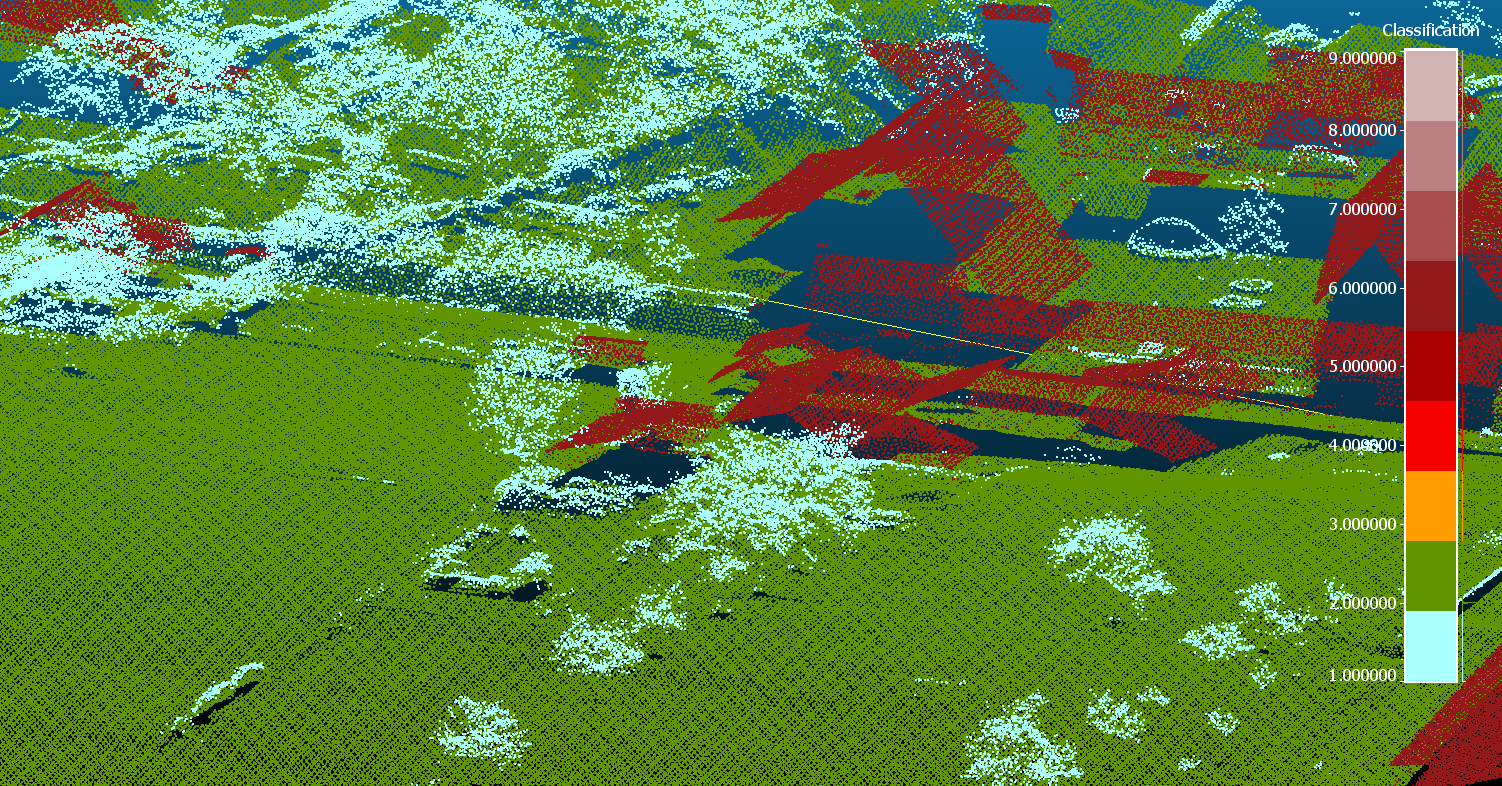
\includegraphics[width=0.7\linewidth]{Figures/heights_3d.png}
    \caption{Vegetation = Tall Trees}
    \label{fig13}
\end{figure}

\noindent Our rationale behind focusing exclusively on trees stems from the assumption that the primary purpose of extracting vegetation from point cloud data is to monitor the health of these trees and to assess their impact on the landscape. By concentrating on trees, we aim to provide more targeted insights into these aspects. Therefore, in this step, our efforts are directed towards developing and implementing a methodology that effectively isolates tree data from the point cloud, distinguishing it from other vegetative and non-vegetative elements.\\

\noindent \textbf{What is Included in 'Unclassified'?}\\
\noindent In our analysis, we delve into understanding the potential composition of the 'unclassified' category in terms of city objects. To facilitate this, we refer to a figure that categorizes city objects as per various common 3D geospatial data formats, such as CityJSON and CityGML. These formats typically define a range of similar categories for representing urban elements.\\

\noindent Comparatively, Table~\ref{table4} delineates the classification system employed by AHN (Actueel Hoogtebestand Nederland). In AHN's framework, certain urban features are categorized distinctly - for instance, utility poles are classified under 'High tension', while roads, tunnels, and bridges fall within the 'Ground' class \citeA{citygml2023} \citeA{cityjson2023} \citeA{geoforum2023} \citeA{leusink2019}.\\

\begin{table}[H]
  \centering
  \caption{Classifications in CityJSON, CityGML, and AHN4}
  \label{table4}
  \small
  \begin{tabular}{c|c|c}
    \hline
    \textbf{CityJSON} & \textbf{CityGML} & \textbf{AHN4} \\
    \Xhline{1pt}
    Bridge & & Ground \\
    \Xhline{0.05pt}
    Building & Building & Building \\
    \Xhline{0.05pt}
    CityFurniture & City furniture & Civil structure/Building/High tension \\
    \Xhline{0.05pt}
    CityObjectGroup & & \\
    \Xhline{0.05pt}
    GenericCityObject & & \\
    \Xhline{0.05pt}
    LandUse & Land use & \\
    \Xhline{0.05pt}
    OtherConstruction & & Ground \\
    \Xhline{0.05pt}
    PlantCover & Vegetation & Unclassified/Ground \\
    \Xhline{0.05pt}
    Solitary VegetationObject & Vegetation & Unclassified \\
    \Xhline{0.05pt}
    TINRelief & Digital Terrain Model & Ground \\
    \Xhline{0.05pt}
    Transportation & Transportation & Ground \\
    \Xhline{0.05pt}
    Tunnel & & Ground \\
    \Xhline{0.05pt}
    WaterBody & Water bodies & Water \\
    \hline
  \end{tabular}
\end{table}

\noindent Taking these classification schemas into account, we postulate that the 'unclassified' category in our dataset likely encompasses a range of objects not specifically categorized by AHN. These may include vegetation (which we are focusing on as tall trees), light poles, cars, and even people. This assumption is pivotal as it guides our methodology in segregating these 'unclassified' objects, particularly in isolating vegetation (trees) from other urban elements that fall into the same category.

\subsubsection{Multiple Methodologies}
In our endeavor to extract vegetation from the provided AHN data, we have conducted a thorough review of methodologies employed in previous research projects. This investigation revealed a diversity of approaches, each leveraging unique aspects of the data and distinct technological advances.\\

\noindent One notable method involves the use of Near-Infrared (NIR) radiation. Vegetation exhibits distinct characteristics when reflecting NIR, making it a potentially effective means for identification. This approach has been effectively utilized in studies by \citeA{xu2020tree} and \citeA{chen2017multispectral}, where NIR reflectance was scanned using Unmanned Aerial Vehicles (UAVs). The success of these studies underscores the viability of NIR-based methods in vegetation detection.\\

\noindent Another approach is density matching, as demonstrated by \citeA{ferrara2018automated}. This method hinges on the analysis of point cloud density, offering a different perspective on vegetation extraction.\\

\noindent Additionally, there is a growing trend in employing machine learning techniques for this task. Pioneering studies by \citeA{carbonell-rivera2024class3dp} and \cite{ozdemir2019aerial} stand out in this domain. These research projects have varied in their feature selection, with some focusing on shape and density, while others incorporate additional dimensions such as RGB color and intensity. The diversity in feature selection reflects the adaptability of machine learning methods to different data characteristics and project goals.\\

\noindent Each of these methods offers unique advantages and potential challenges. Their effectiveness can vary based on the specific characteristics of the dataset and the objectives of the study. Therefore, in selecting a method for our project, we will consider these factors to determine the most suitable approach for extracting vegetation from the AHN data.\\


\begin{table}[H]
  \centering
  \small
  \caption{Pros and Cons of Different Methods}
  \label{table:methods-pros-cons}
  \renewcommand{\arraystretch}{1.5}  
  \begin{tabular}{|l|p{5cm}|p{5cm}|}
    \hline
    \textbf{Method} & \textbf{Pros} & \textbf{Cons} \\
    \hline
    Use NIR & 
    \begin{itemize}
      \item It takes full advantage of vegetation’s characteristics..
    \end{itemize} & 
    \begin{itemize}
      \item Resolution does matter.
      \item It contains all kinds of vegetation, which isn’t the best for our case; grasses and cropland are classified as ground.
    \end{itemize} \\
    \hline
    Machine learning & 
    \begin{itemize}
      \item It may have great accuracy even classifying from scratch.
    \end{itemize} & 
    \begin{itemize}
      \item Need to prepare training data, and polite parameter tuning is needed.
      \item More than our current knowledge.
    \end{itemize} \\
    \hline
  \end{tabular}
\end{table}

\noindent Regarding the approach using Near-Infrared (NIR) data, we initially considered its potential application. However, upon closer examination, we concluded that it might not be viable for our specific case. The main concern lies in the resolution of NIR raster data. As illustrated in Figure~\ref{nir} showing the Sentinel 2 False color image, the resolution does not appear sufficient to classify individual points accurately. This limitation could significantly hinder our ability to distinguish between different types of vegetation or other city objects.\\

\noindent Turning our attention to machine learning approaches, we recognized their potential for high performance in classifying city objects. However, considering the context of our project, where the AHN data has already classified most city objects, employing a complex machine learning model might be excessive for our needs. It could introduce unnecessary complexity without proportionate benefits, especially given the already high level of classification detail in AHN data.\\

\noindent Therefore, after weighing the pros and cons of these methods, we decided to explore two different approaches. These approaches are selected based on their feasibility, the nature of our data, and the specific objectives of our project. Our goal is to find a balance between accuracy, efficiency, and the practicality of implementation, ensuring that the chosen methods are well-suited to extract vegetation effectively from the AHN data.\\

\begin{figure}[H]
    \centering
    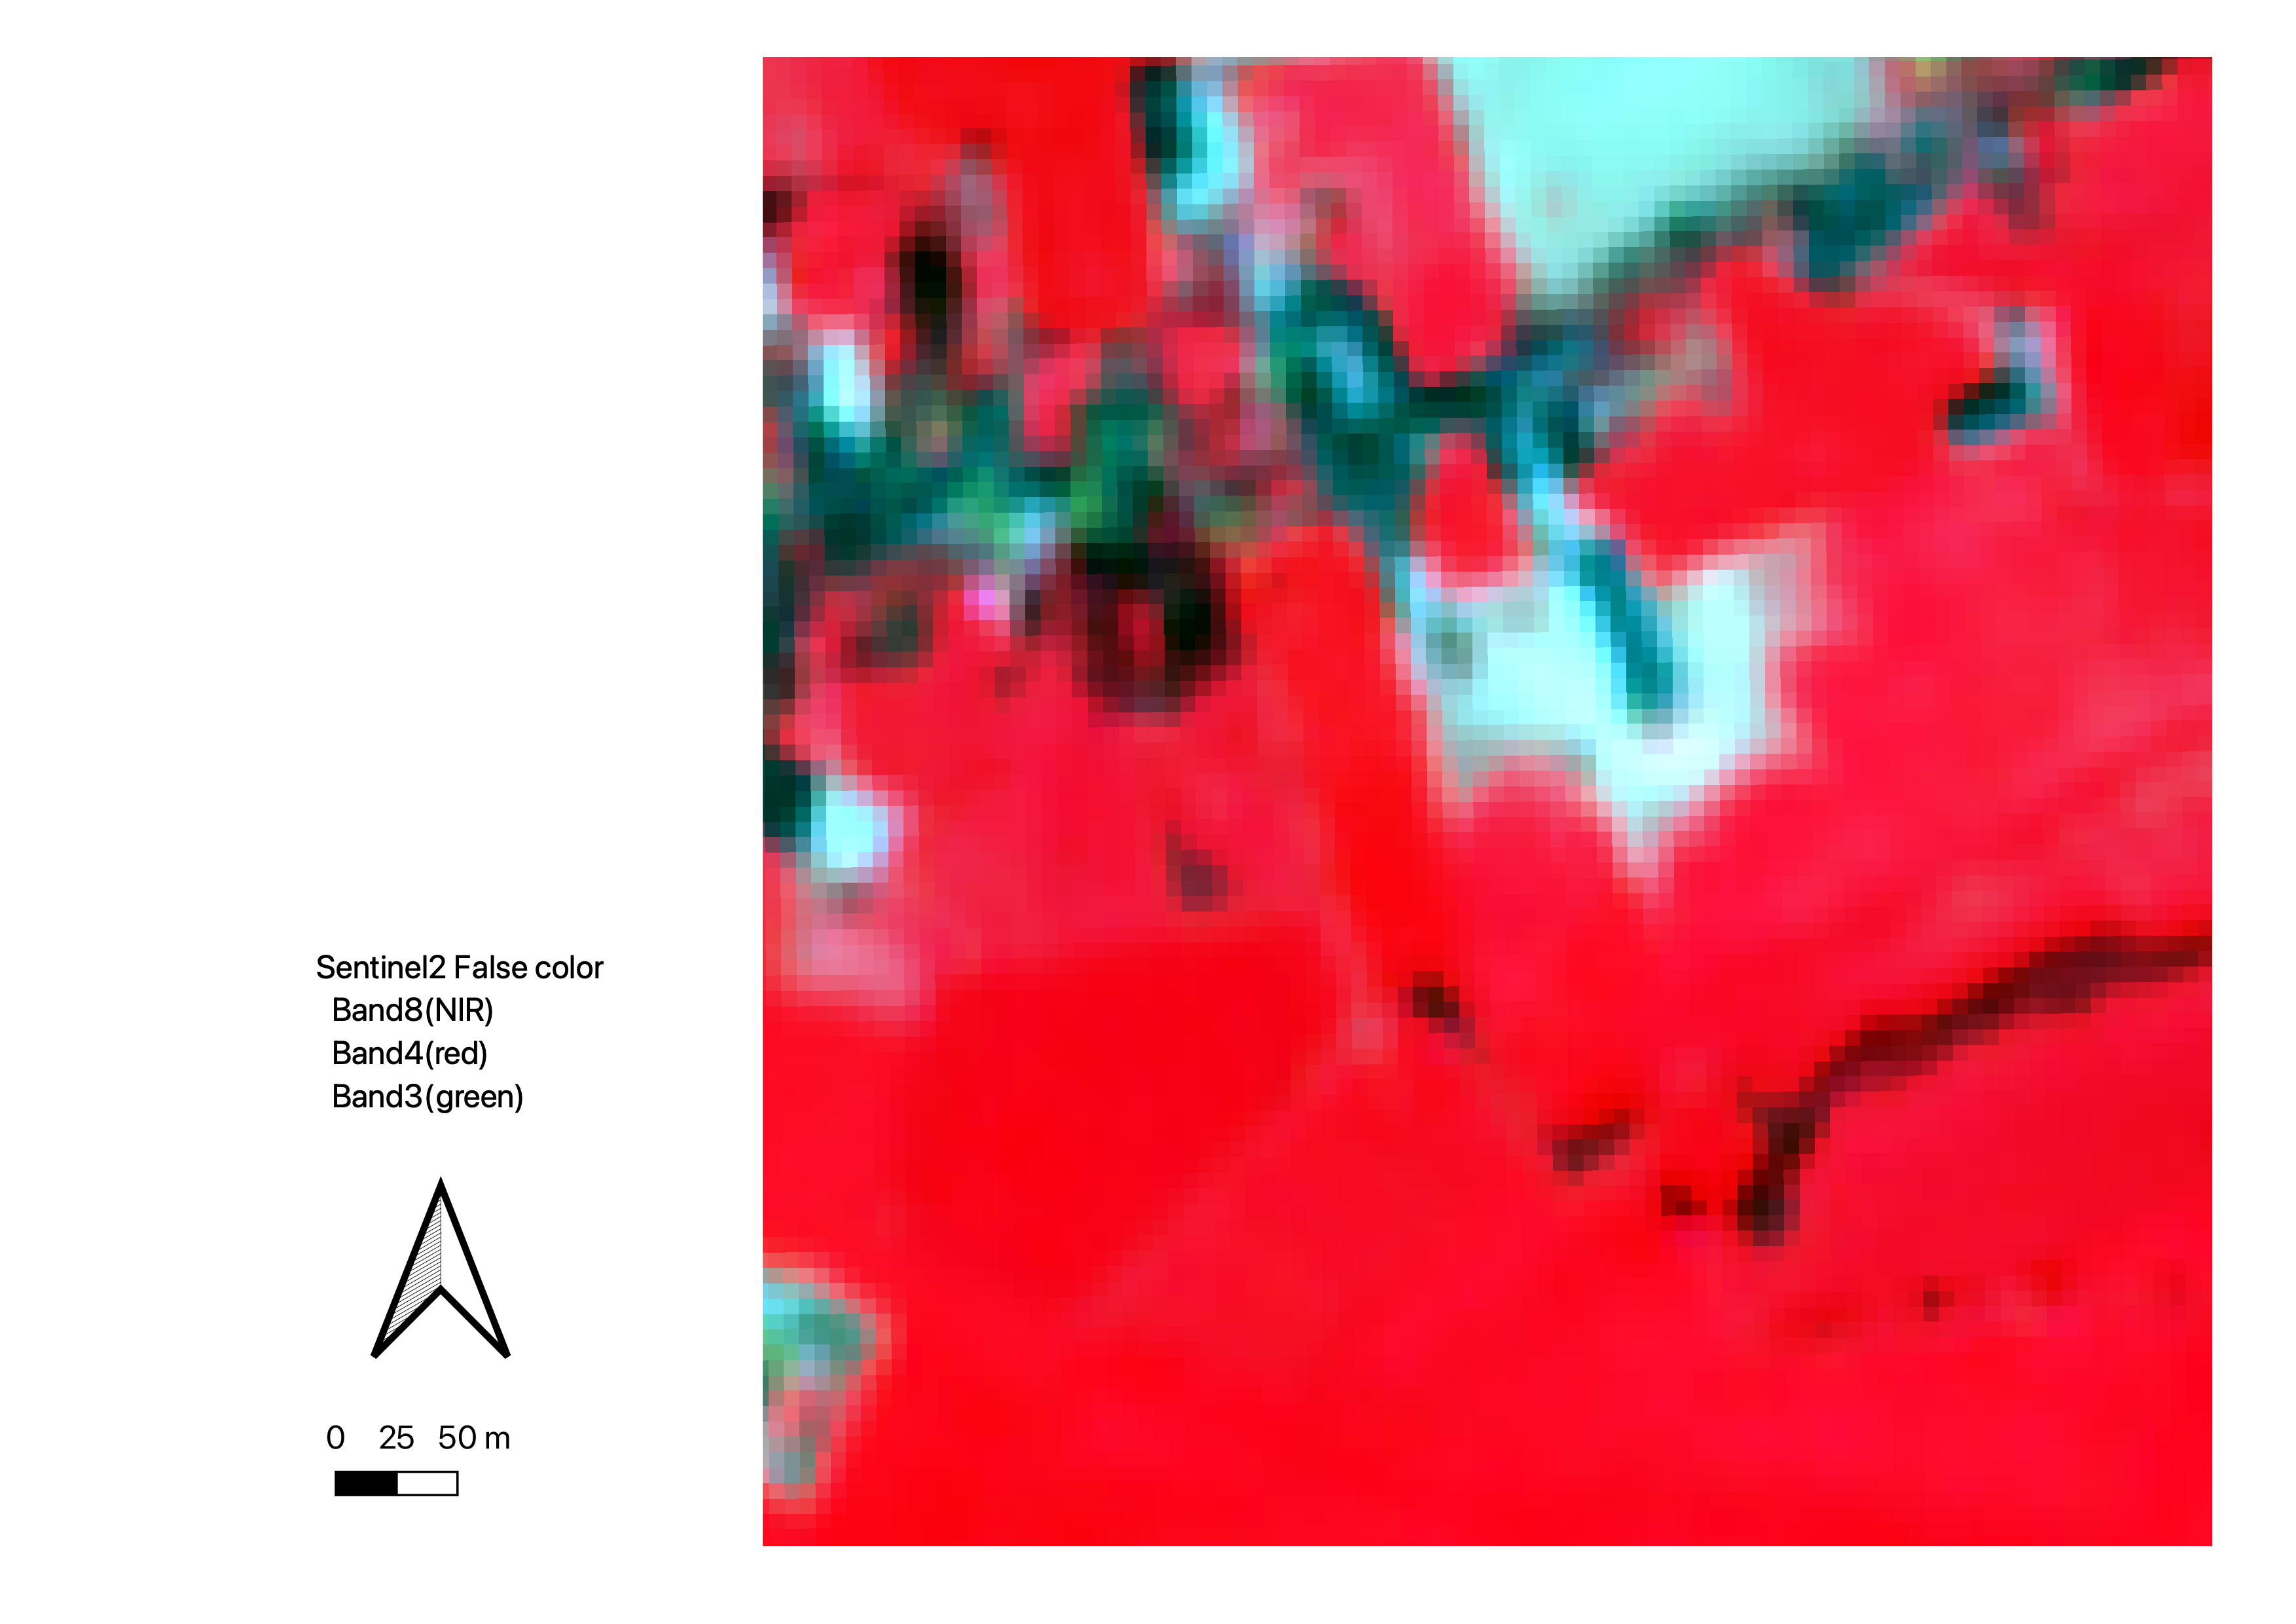
\includegraphics[width=0.7\linewidth]{Figures/nir.png}
    \caption{Sentinel 2 False Color Image}
    \label{nir}
\end{figure}

\subsubsection{Our Approach}
\noindent \textbf{Using Number of Returns and DBSCAN}\\
\noindent The first approach we employed combines the use of DBSCAN clustering with an analysis of the number of returns from the LiDAR data. DBSCAN, or Density-Based Spatial Clustering of Applications with Noise, is particularly adept at identifying clusters based on the density of points. By implementing DBSCAN as the initial step, we effectively isolate denser clusters, allowing us to eliminate smaller, less significant clusters. These smaller clusters often represent low-lying vegetation or other forms of noise that are not our primary focus.\\

\noindent Following the clustering, the next stage involves filtering out clusters with a lower number of returns. The rationale behind this is that taller trees are more likely to have a higher number of returns due to the reflection of radio waves by their leaves and branches. This characteristic becomes a critical filter, enabling us to exclude objects that do not meet the criteria, such as cars, people, and low-lying vegetation like bushes.\\

\noindent Having isolated the clusters likely to represent taller trees, we then focus on extracting the vegetation surface. For this, we consider only the first return from the remaining tree clusters, as this is most representative of the uppermost vegetation layer. The final step in this approach is the rasterization process, where we extract the highest point within each grid cell. This method allows us to create a more accurate representation of the tree canopy, which is our primary target in extracting vegetation from the AHN data.\\

\noindent\textbf{Intensity}\\
\noindent The second approach attempted uses intensity scores of the LiDAR data. Intensity is recorded as the strength of each return per scan. To implement this step, we firstly filtered for unclassified points using PDAL. In return, this gives us all points of vegetation and other unclassified points such as lamp posts, cars or unidentified buildings. We then filtered the points in a range where the intensity values cover vegetation. After inspection of the data, it indicated that lower intensity values can be classified as vegetation and higher values are the other unclassified objects. This is due to factors such as surface material, absorption and the number of returns. Surface materials affect the intensity as organic material, tree leaves, in this case, tend to scatter the laser light more in multiple directions. Leaves and other vegetation also tend to absorb more of the laser beams in certain wavelengths giving lower overall intensity values. Finally, as trees will have more canopy levels, there will be a higher number of returns. With each reflection, the intensity value lowers the laser signal strength also giving lower intensity values.\\

\noindent Initially, we implemented a hardcoded range where we filtered for a range of 0 to 900. This gave good results as the overall range of our given AHN4 tile was approximate from 0 to 2500, as shown in the histogram in Figure~\ref{histogram}. The fitlered result in shown in Figure~\ref{filterintensity}. However, further testing in different tiles, it was clear that the range of the given values was not the same for each tile. This meant that selecting a range of 0 to 900 would not work in every tile.


\begin{figure}[H]
    \centering
    \subfloat[Range of Intensity in Our Tile]{%
        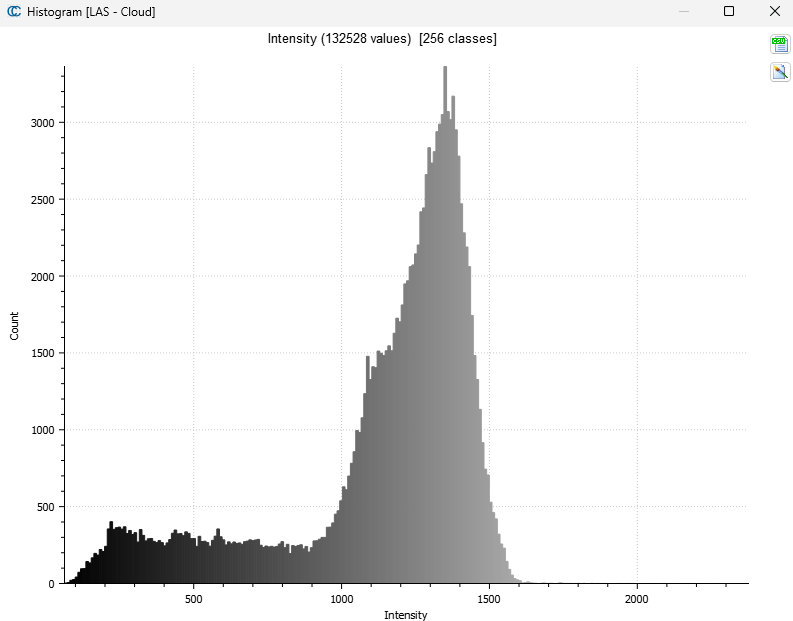
\includegraphics[width=0.4\linewidth]{Figures/histogram.png}
        \label{histogram}
    }
    \hspace{0.5cm}
    \subfloat[Filtered Result Using Intensity]{%
        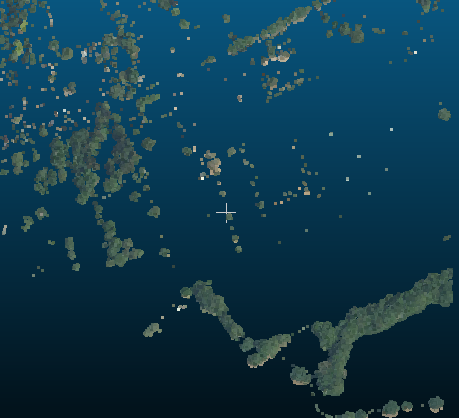
\includegraphics[width=0.4\linewidth]{Figures/veg_filter.png}
        \label{filterintensity}
    }
    \caption{Intensity Application for Filtering}
    \label{fig:comparison}
\end{figure}

\noindent Additionally, further research indicated that intensity values can be affected by a wider range of factors. Different measuring instruments will give a different scale of intensity compared to the 0 to 2500 in our dataset. This can be due to the calibration of the measuring instrument, angle of scanning, atmospheric conditions, and wavelength of the laser \citeA{lackova2023unlocking}.\\

\noindent To implement this in a way that will filter the data for different datasets, we attempted to normalise the data. Our first attempt at normalising the data was converting the range into a linear function. This method allowed us to filter the bottom 30 to 40\% of the range for every dataset. For our thinned point cloud, this yielded a good result as we can see in Figure~\ref{filterintensity}.  However, when testing with the bigger area of the original point cloud data (before cropping to 500x500), it showed that it did not filter as well. We can see Figure~\ref{fullintensity} showing the results that there are many other unclassified buildings or street furniture included.\\

\begin{figure}[H]
    \centering
    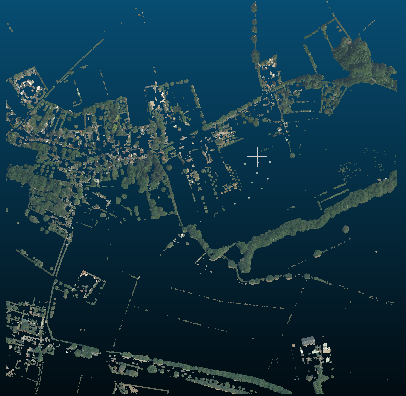
\includegraphics[width=0.5\linewidth]{Figures/fullintensity.png}
    \caption{Intensity Range Applied to Bigger Area of the Pointcloud Tile}
    \label{fullintensity}
\end{figure}

\noindent Another statistical method to normalize and filter the data range attempted was calculating the z-scores and creating a z-score range that can successfully filter for our designated vegetation points only. Z scores describe the intensities’ relationship to the mean in our group of values. The z score is measured in number of standard deviations to the mean.  Z is the Z score, X is the Intensity, $\mu$ is the mean of the group of values and $\sigma$ is the standard deviation of the group of values.\\

\[Z = (X - \mu )/ \sigma\]

\noindent When testing different Z score ranges to implement, again, it gave good results in our thinned dataset in Figure~\ref{ournormalised} , but not a bigger area as seen in Figure~\ref{ourfulltile} and Figure~\ref{othersfulltile} respectively.\\


% \begin{figure}[H]
%     \centering
%     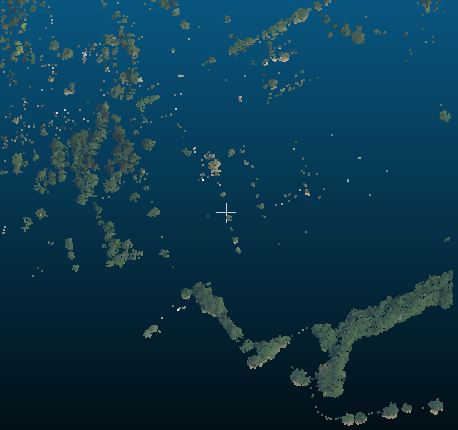
\includegraphics[width=0.5\linewidth]{Figures/ournormalized.png}
%     \caption{Vegetation Filtering on Cropped Tile Using Normalized Intensity}
%     \label{ournormalised}
% \end{figure}

% \begin{figure}[H]
%     \centering
%     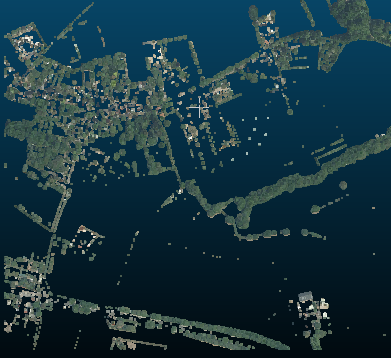
\includegraphics[width=0.5\linewidth]{Figures/ourfulltile.png}
%     \caption{Vegetation Filtering on Bigger Area Using Normalized Intensity}
%     \label{ourfulltile}
% \end{figure}

\begin{figure}[H]
    \centering
    \subfloat[Vegetation Filtering on Cropped Tile Using Normalized Intensity]{%
        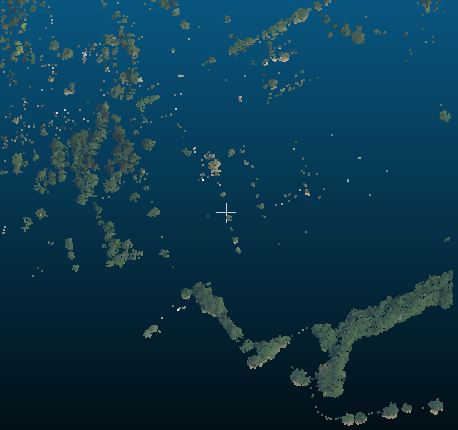
\includegraphics[width=0.4\linewidth]{Figures/ournormalized.png}
        \label{ournormalised}
    }
    \hspace{0.5cm}
    \subfloat[Vegetation Filtering on Bigger Area Using Normalized Intensity]{%
        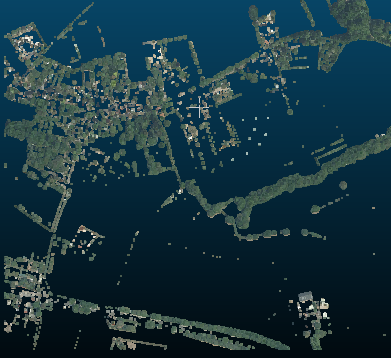
\includegraphics[width=0.4\linewidth]{Figures/ourfulltile.png}
        \label{ourfulltile}
    }
    \caption{Intensity Application for Filtering}
    \label{fig:comparison}
\end{figure}

\begin{figure}[H]
    \centering
    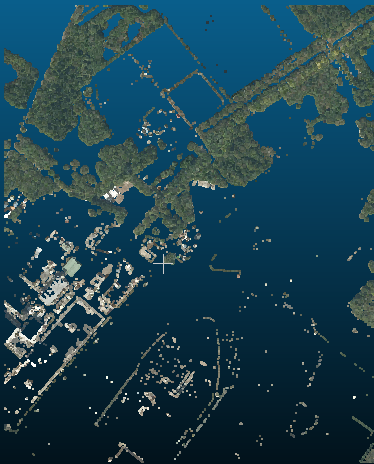
\includegraphics[width=0.4\linewidth]{Figures/othersfultile.png}
    \caption{Vegetation Filtering on Bigger Area Using Normalized Intensity (other dataset)}
    \label{othersfulltile}
\end{figure}


\subsubsection{Evaluation}
\noindent \textbf{Number of Returns}\\
\noindent The following four figures provide a visual demonstration of how each step in our process contributes effectively towards achieving our key objectives. Figure~\ref{beforedbscan} and Figure~\ref{afterdbscan} display the point cloud data before and after the application of the DBSCAN clustering algorithm, respectively. In Figure~\ref{beforedbscan}, we observe the original distribution of point clouds, including various tiny clusters. After applying DBSCAN, as shown in Figure~\ref{afterdbscan}, there is a noticeable reduction in these small clusters. This change indicates the effectiveness of DBSCAN in filtering out elements that we do not classify as trees, which are likely to be bushes or mounds of sand. The algorithm's ability to discriminate between tree-like structures and smaller, less significant clusters is clearly evident.\\

\noindent Figure~\ref{beforenumofreturn} and Figure~\ref{afternumofreturn} further illustrate the process, showing the point cloud data before and after filtering based on the number of returns. Figure~\ref{beforenumofreturn} presents the data with all features intact, while Figure~\ref{afternumofreturn} reveals the data post-filtering. The latter figure exhibits a significant reduction in features that do not resemble trees. This outcome confirms the success of our approach in isolating tree structures from the point cloud data. The filtering process effectively removes non-tree elements, leaving behind a cleaner and more focused representation of the tree canopy.\\

\noindent These visual comparisons serve as a compelling testament to the efficacy of our methodologies. Each step, from DBSCAN clustering to filtering based on returns, plays a crucial role in refining the data and aligning it more closely with our objective of accurately extracting tree structures from the point cloud data.\\


\begin{figure}[H]
    \centering
    \subfloat[Before Running DBSCAN]{%
        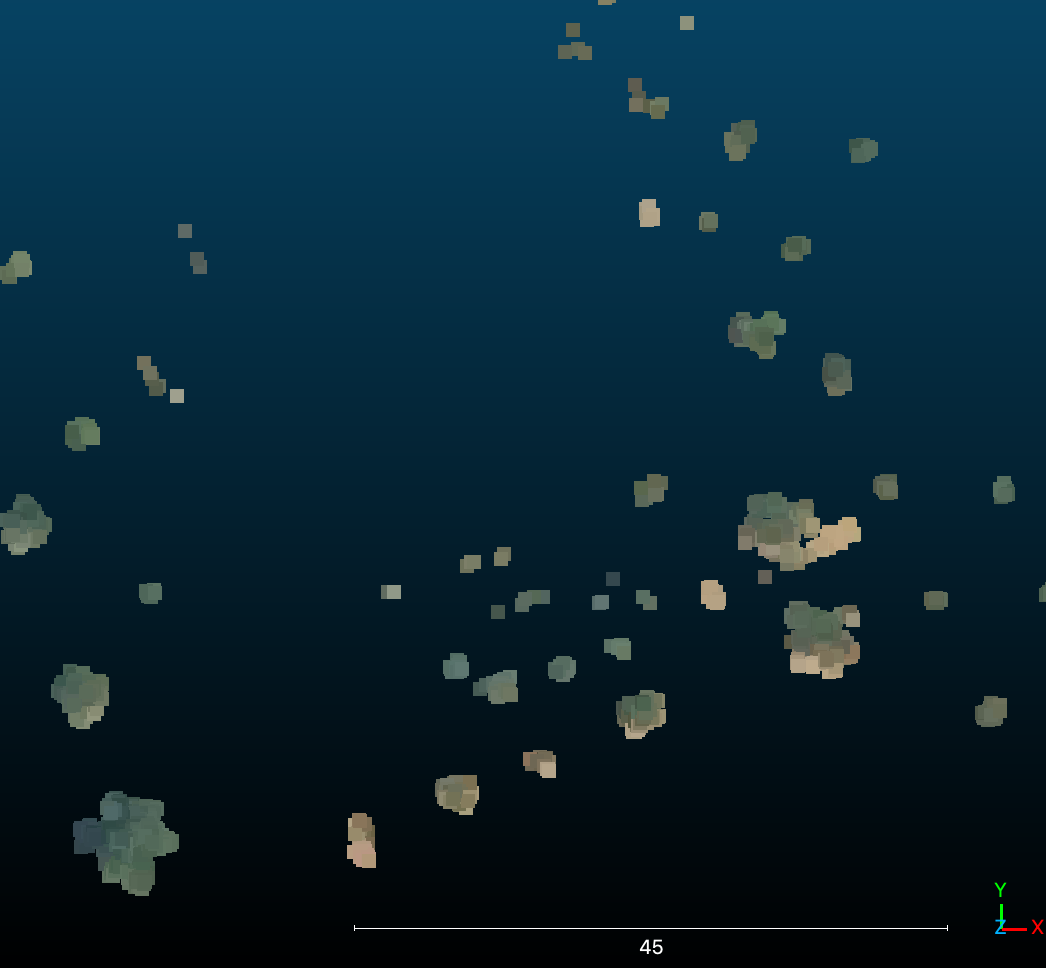
\includegraphics[width=0.4\linewidth]{Figures/beforedbscan.png}
        \label{beforedbscan}
    }
    \hspace{0.5cm}
    \subfloat[After Running DBSCAN]{%
        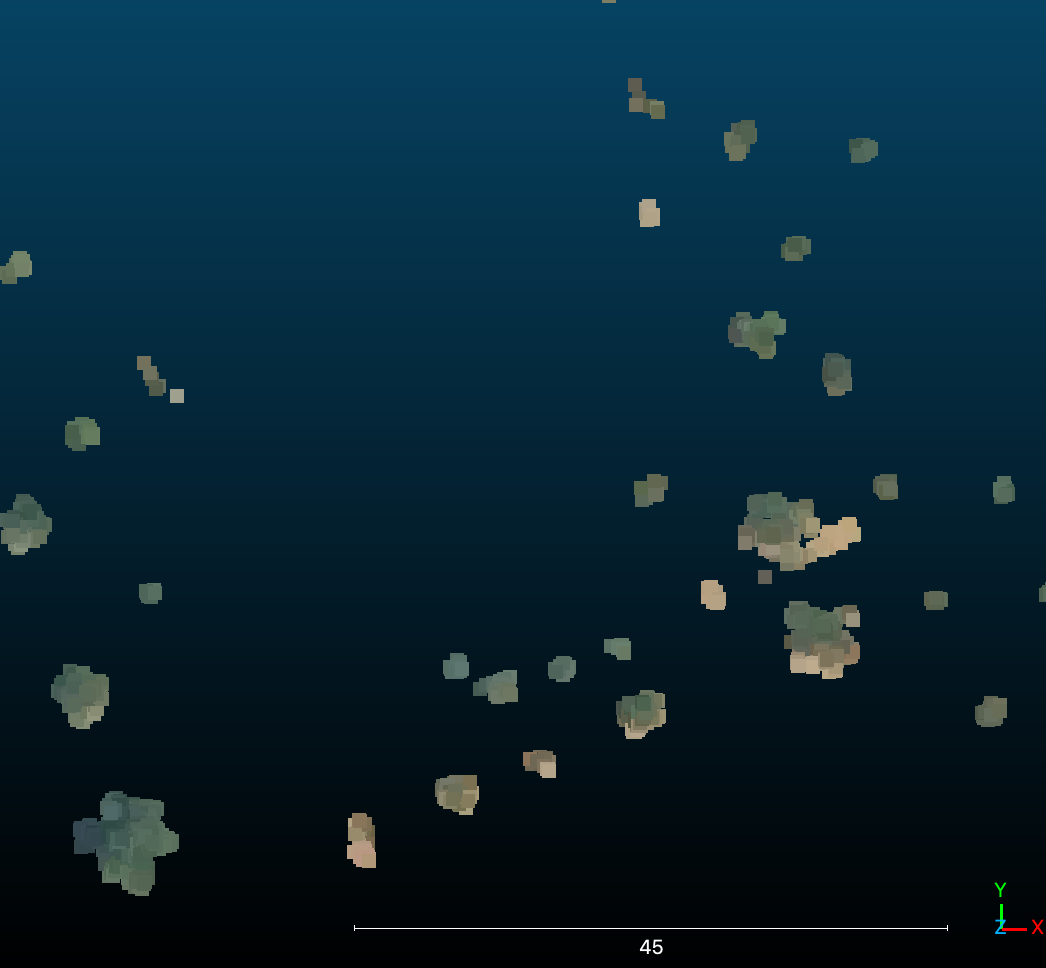
\includegraphics[width=0.4\linewidth]{Figures/afterdbscan.png}
        \label{afterdbscan}
    }
    \caption{DBSCAN Implementation}
    \label{fig:comparison}
\end{figure}


\begin{figure}[H]
    \centering
    \subfloat[Before Filtering by Number of Returns]{%
        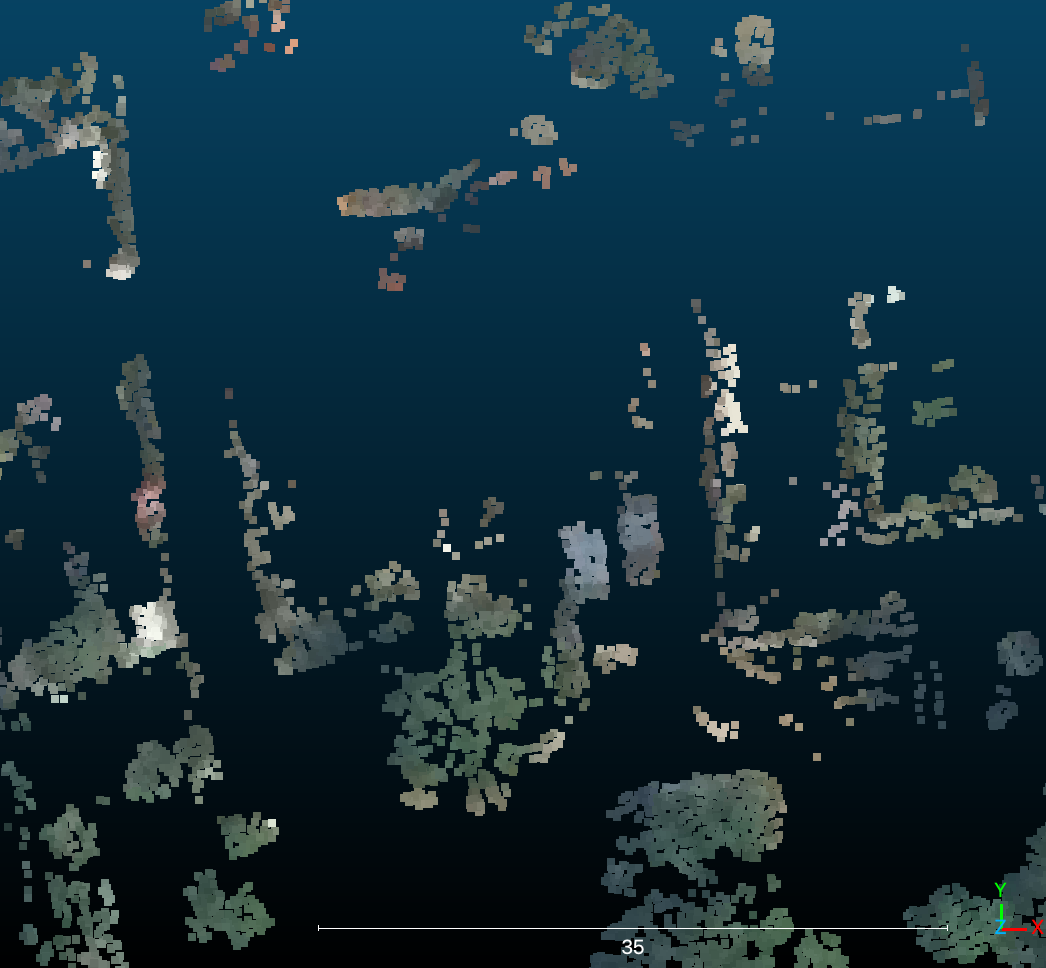
\includegraphics[width=0.4\linewidth]{Figures/beforenumofreturn.png}
        \label{beforenumofreturn}
    }
    \hspace{0.5cm}
    \subfloat[After Filtering by Number of Returns]{%
        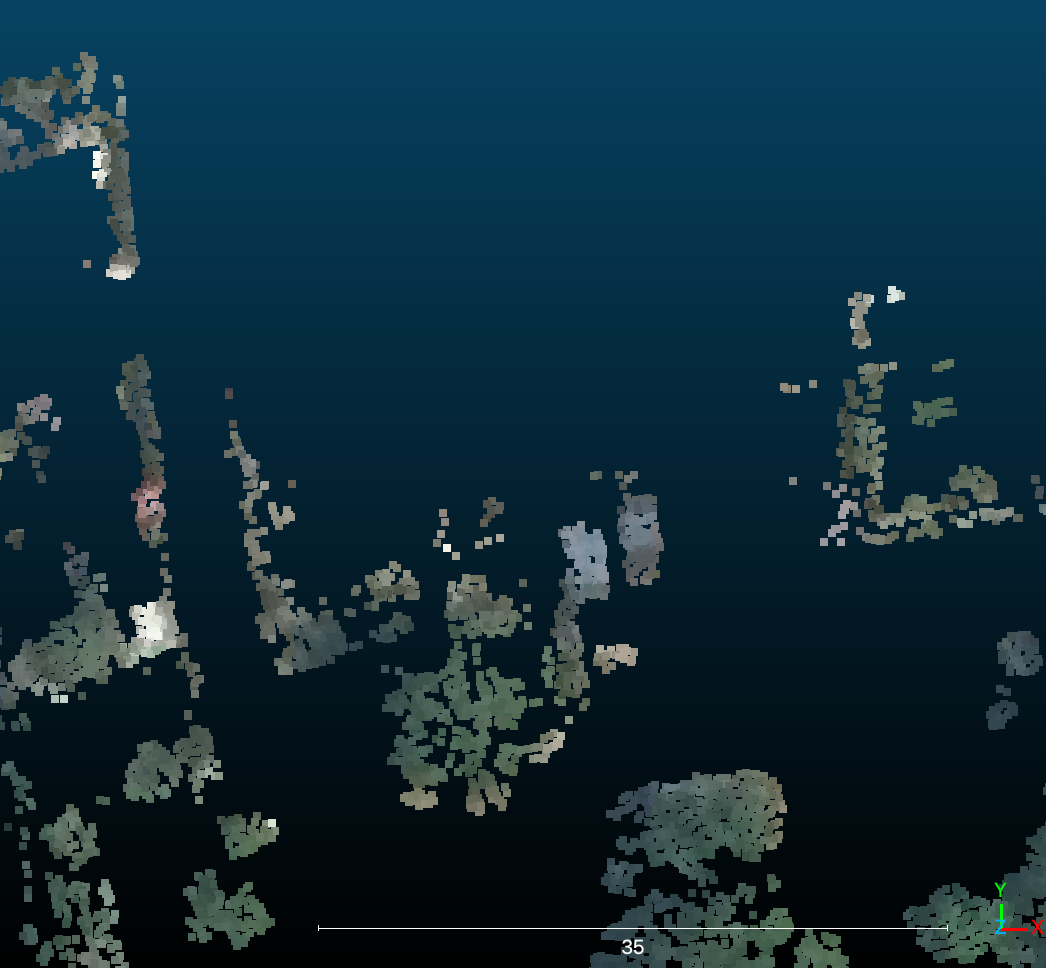
\includegraphics[width=0.4\linewidth]{Figures/afternumofreturn.png}
        \label{afternumofreturn}
    }
    \caption{Number-of-Returns Implementation}
    \label{fig:comparison}
\end{figure}

\noindent In evaluating our approach to extracting tall trees from the 'unclassified' classes in AHN data, we conducted a comparison with aerial photographs provided by AHN. Figure~\ref{vege}, Figure~\ref{vegwithdtm} and Figure~\ref{vegwithaerial} play a crucial role in this evaluation, showcasing how our extracted vegetation data overlaps with the aerial imagery. As evident from the figure, our program demonstrates a commendable capability in identifying vegetation areas. The overlay of extracted vegetation on the aerial photo indicates that densely forested areas are particularly well-represented by our method.\\

\noindent Upon closer inspection, as highlighted in Figure~\ref{vegwithaerial}, it is observed that our approach successfully discriminates between tall trees and other 'unclassified' city objects, such as cars. This effective exclusion of non-vegetative elements reaffirms the precision of our methodology.\\

\begin{figure}[H]
    \centering
    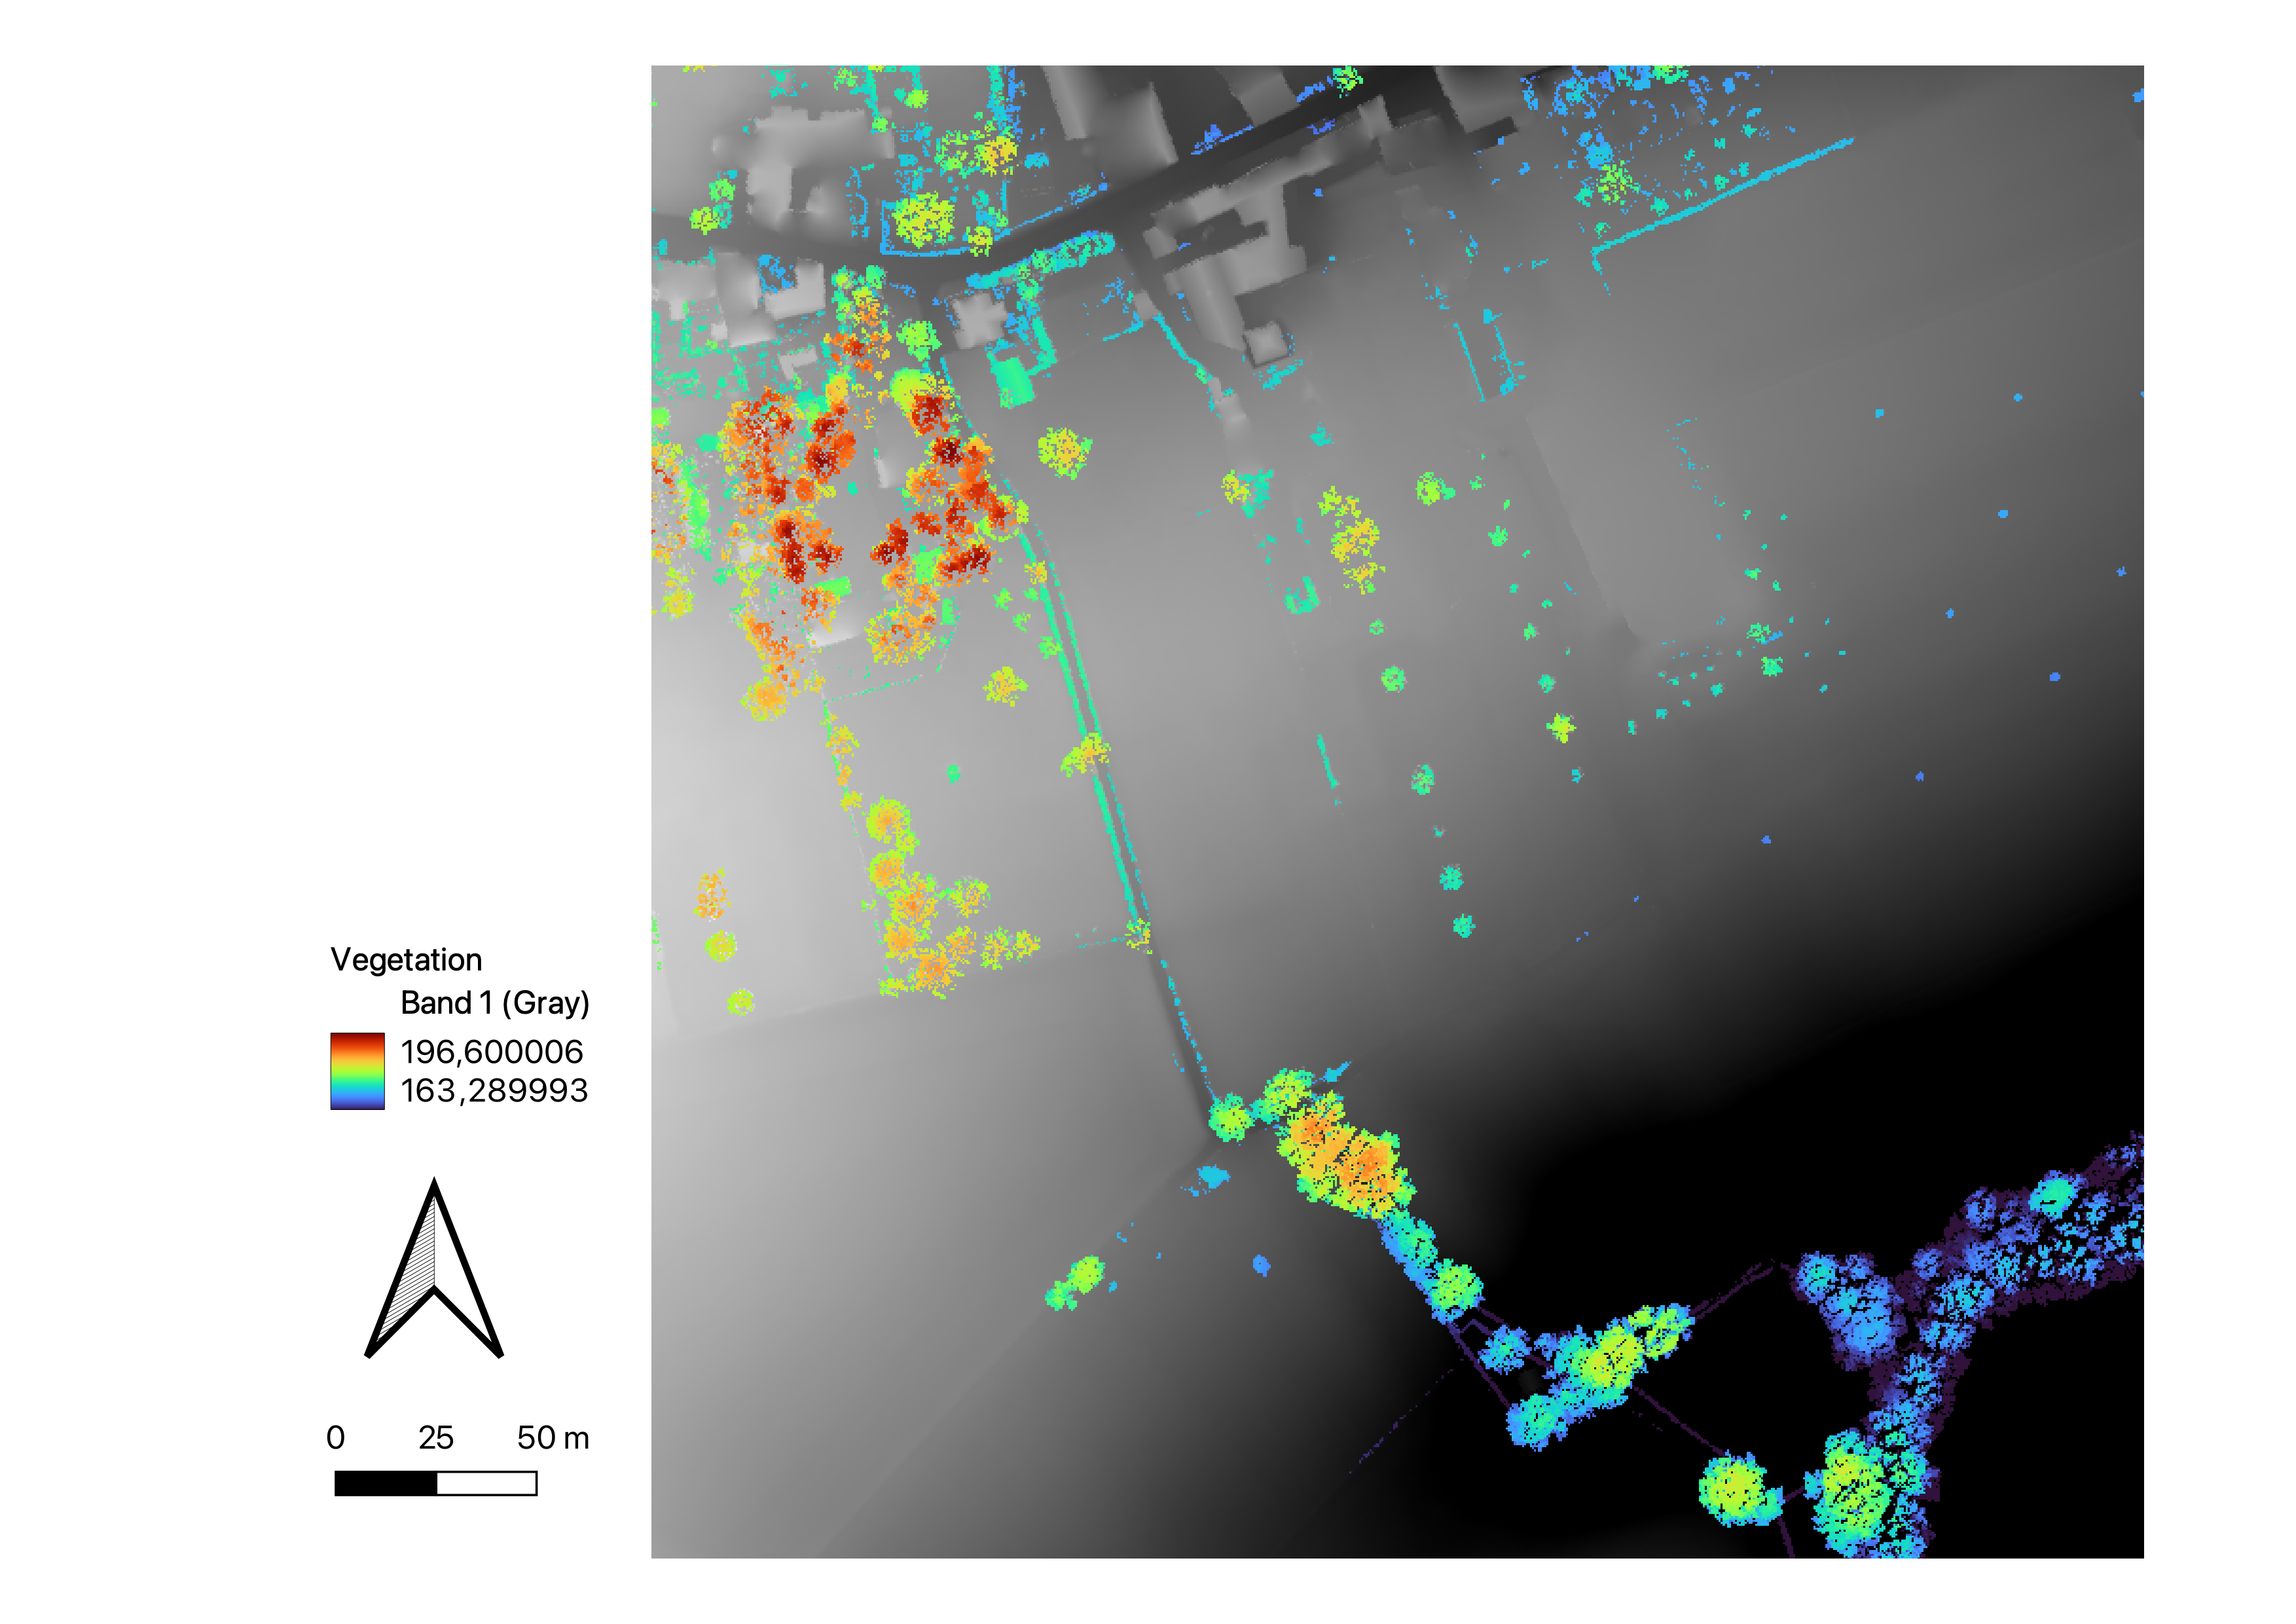
\includegraphics[width=0.7\linewidth]{Figures/vegetation.png}
    \caption{Extracted Vegetation Points Using Number of Returns}
    \label{vege}
\end{figure}


\begin{figure}[H]
    \centering
    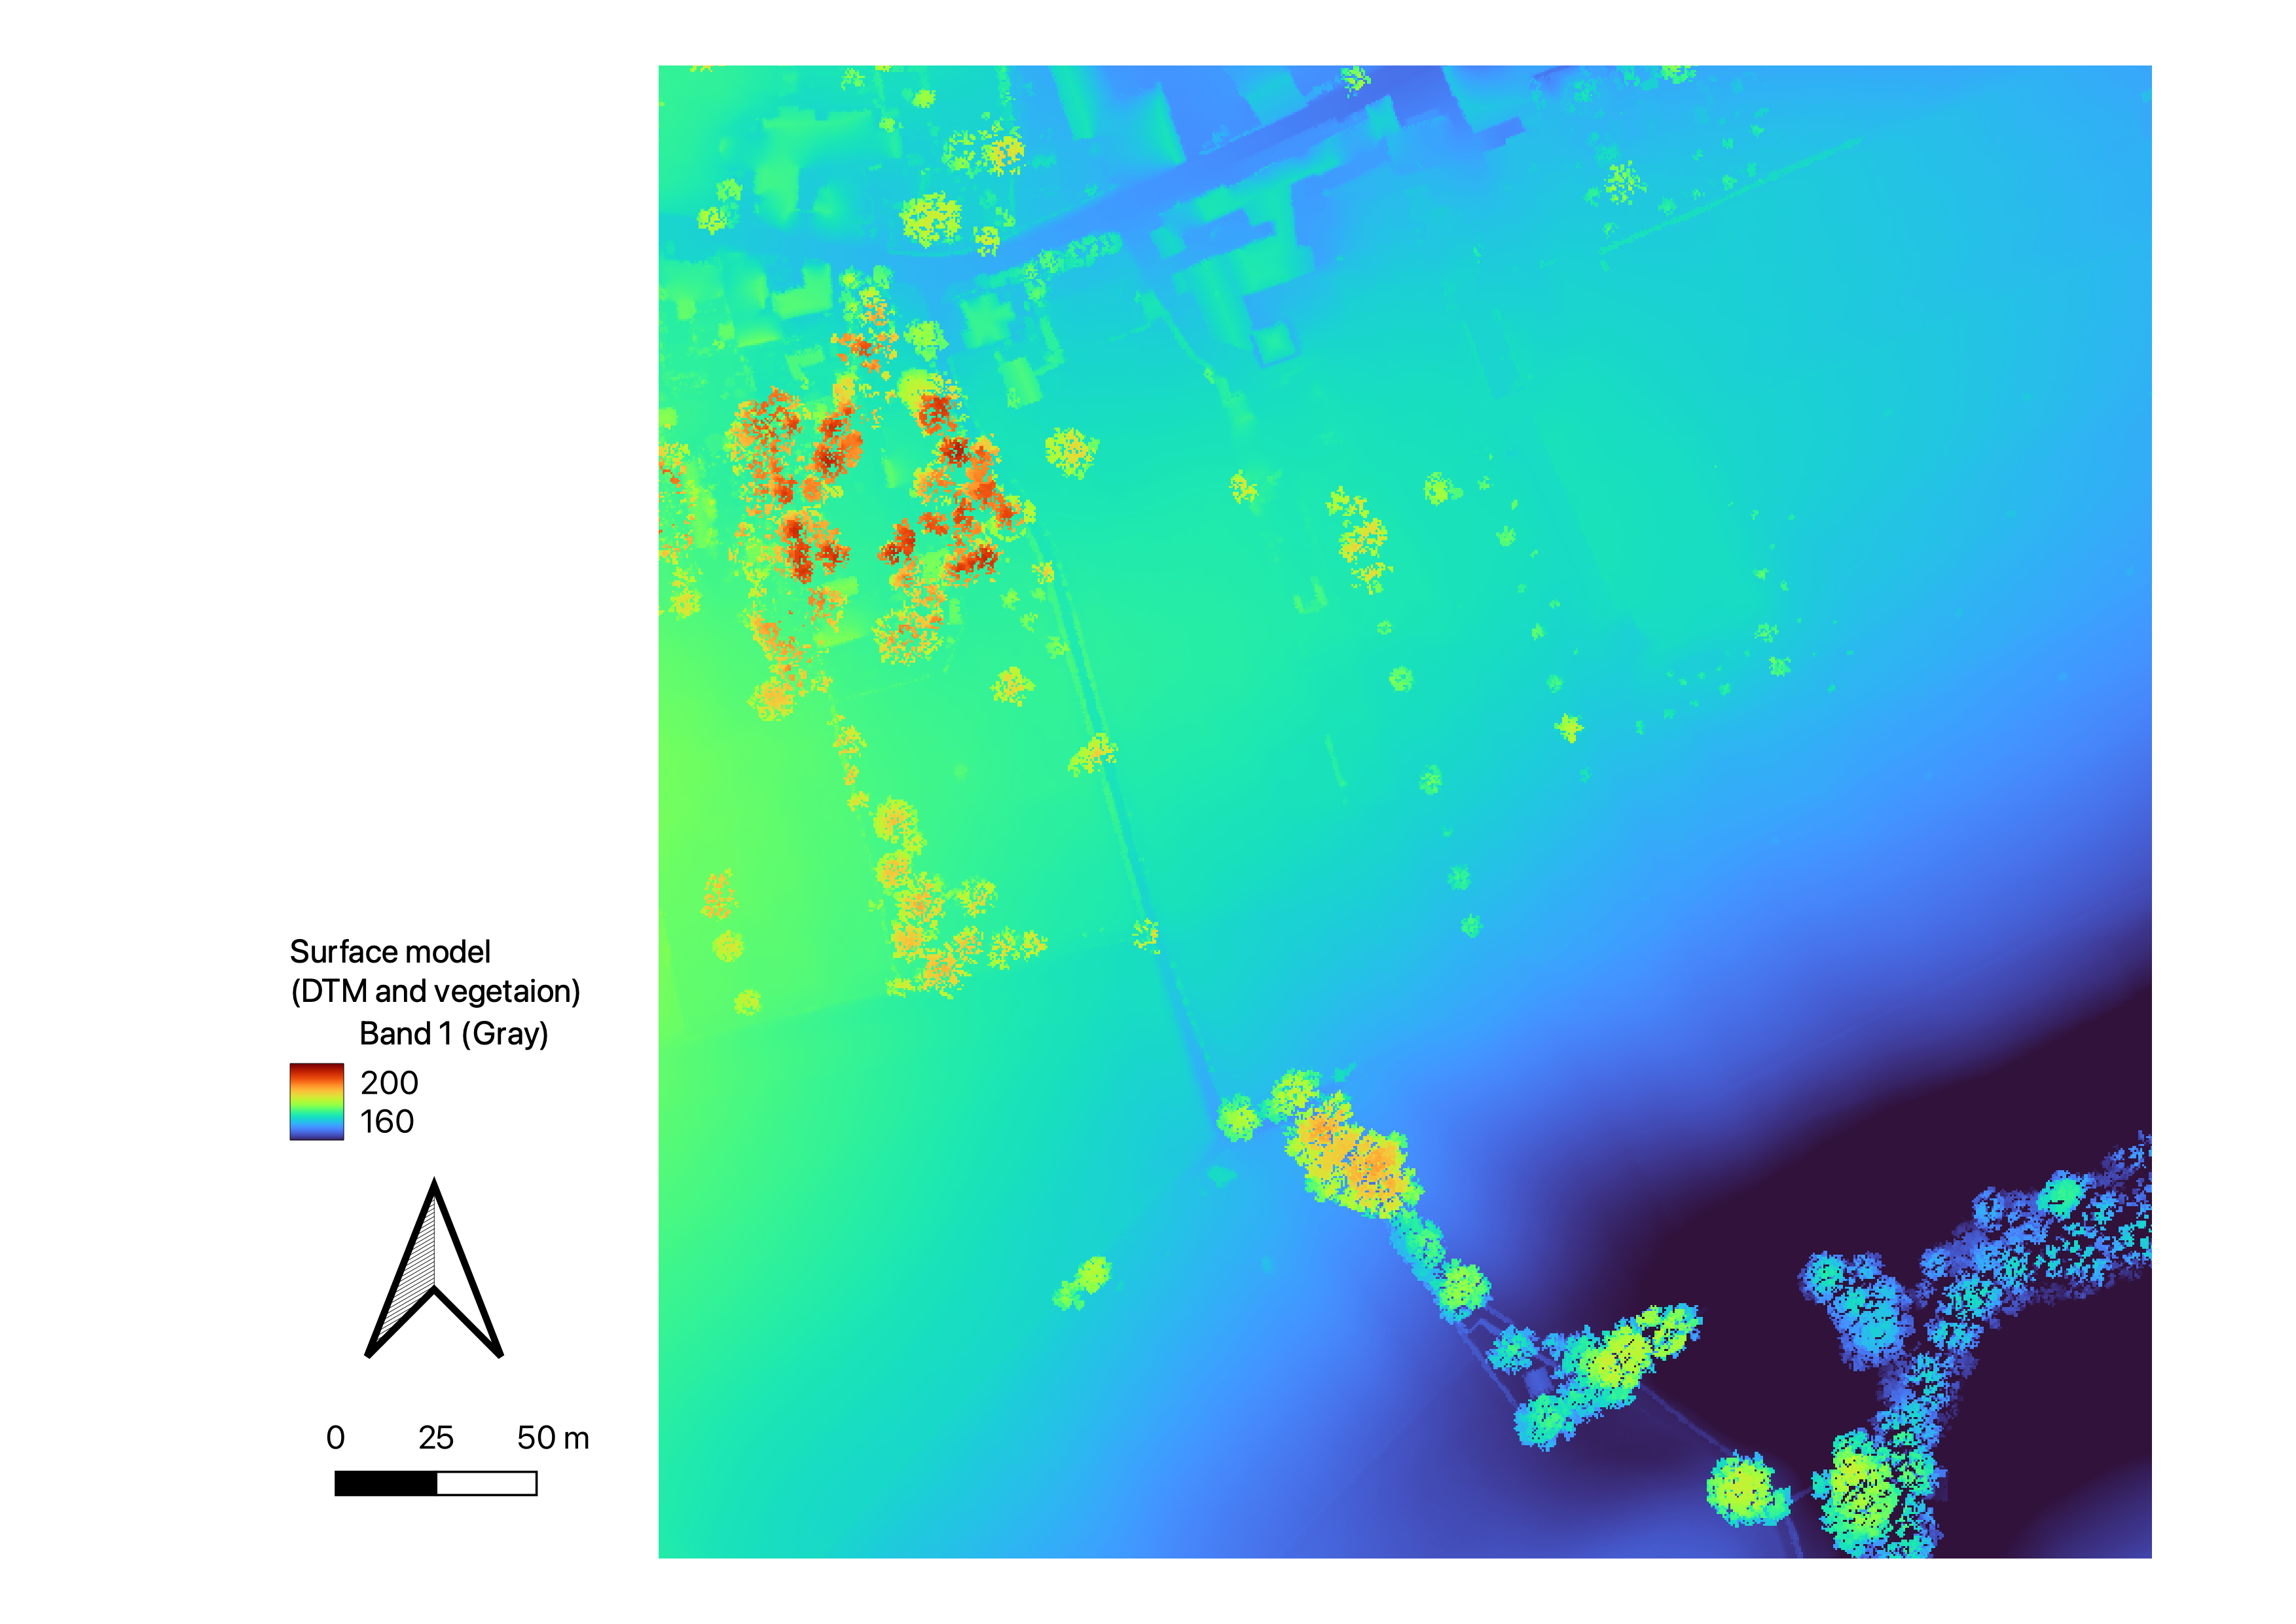
\includegraphics[width=0.7\linewidth]{Figures/vegeation and DTM.png}
    \caption{Extracted Vegetation Points on DTM}
    \label{vegwithdtm}
\end{figure}

\begin{figure}[H]
    \centering
    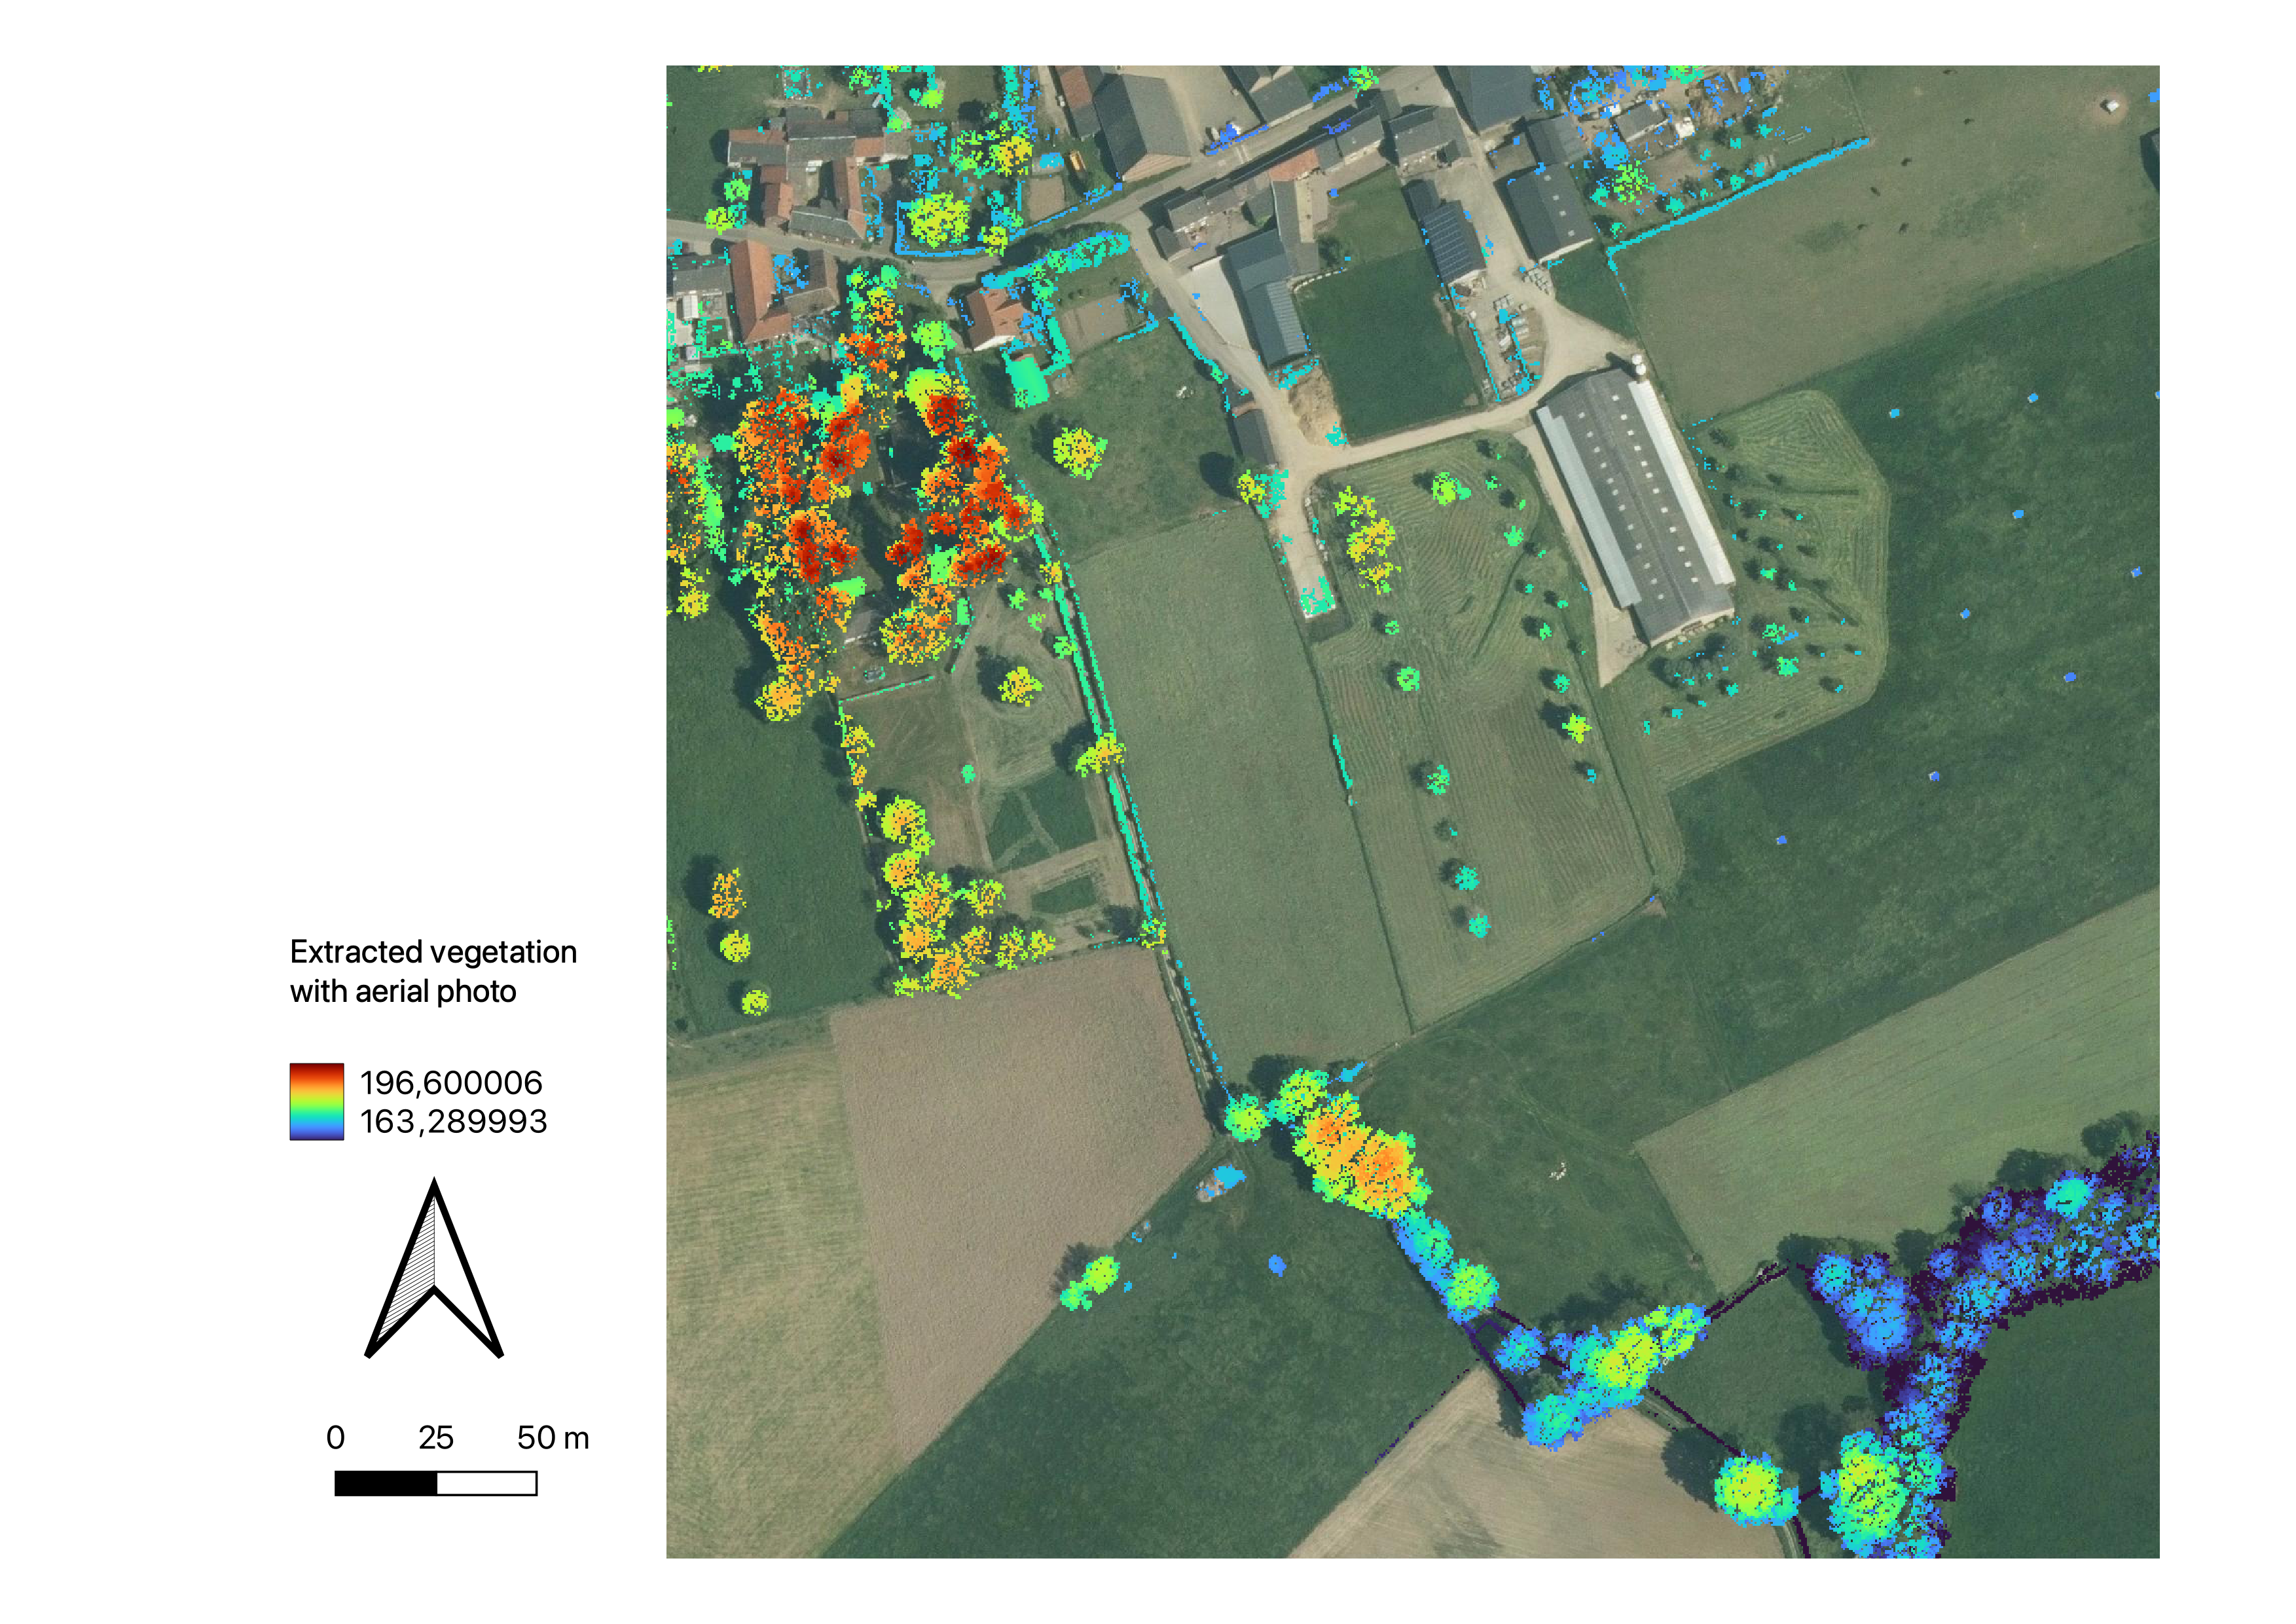
\includegraphics[width=0.7\linewidth]{Figures/vegetation on aerial.png}
    \caption{Extracted Vegetation Point on Aerial Photo}
    \label{vegwithaerial}
\end{figure}

\noindent However, we have identified areas for improvement. One significant issue is the handling of empty pixels within tree clusters. According to the specifications of the AHN point cloud data, as noted by the 3D Geoinformation Research Group, the average density is approximately 8 points per square meter. Given that our target raster data resolution is 0.5 meters per pixel, and considering our implementation of a 50\% thinning process to reduce data size, it's conceivable that some 0.5-meter square grids may have fewer points. Consequently, this can lead to empty pixels even within areas classified as vegetation. This is illustrated in Figure~\ref{numofreturnsimprovement}.\\

\begin{figure}[H]
    \centering
    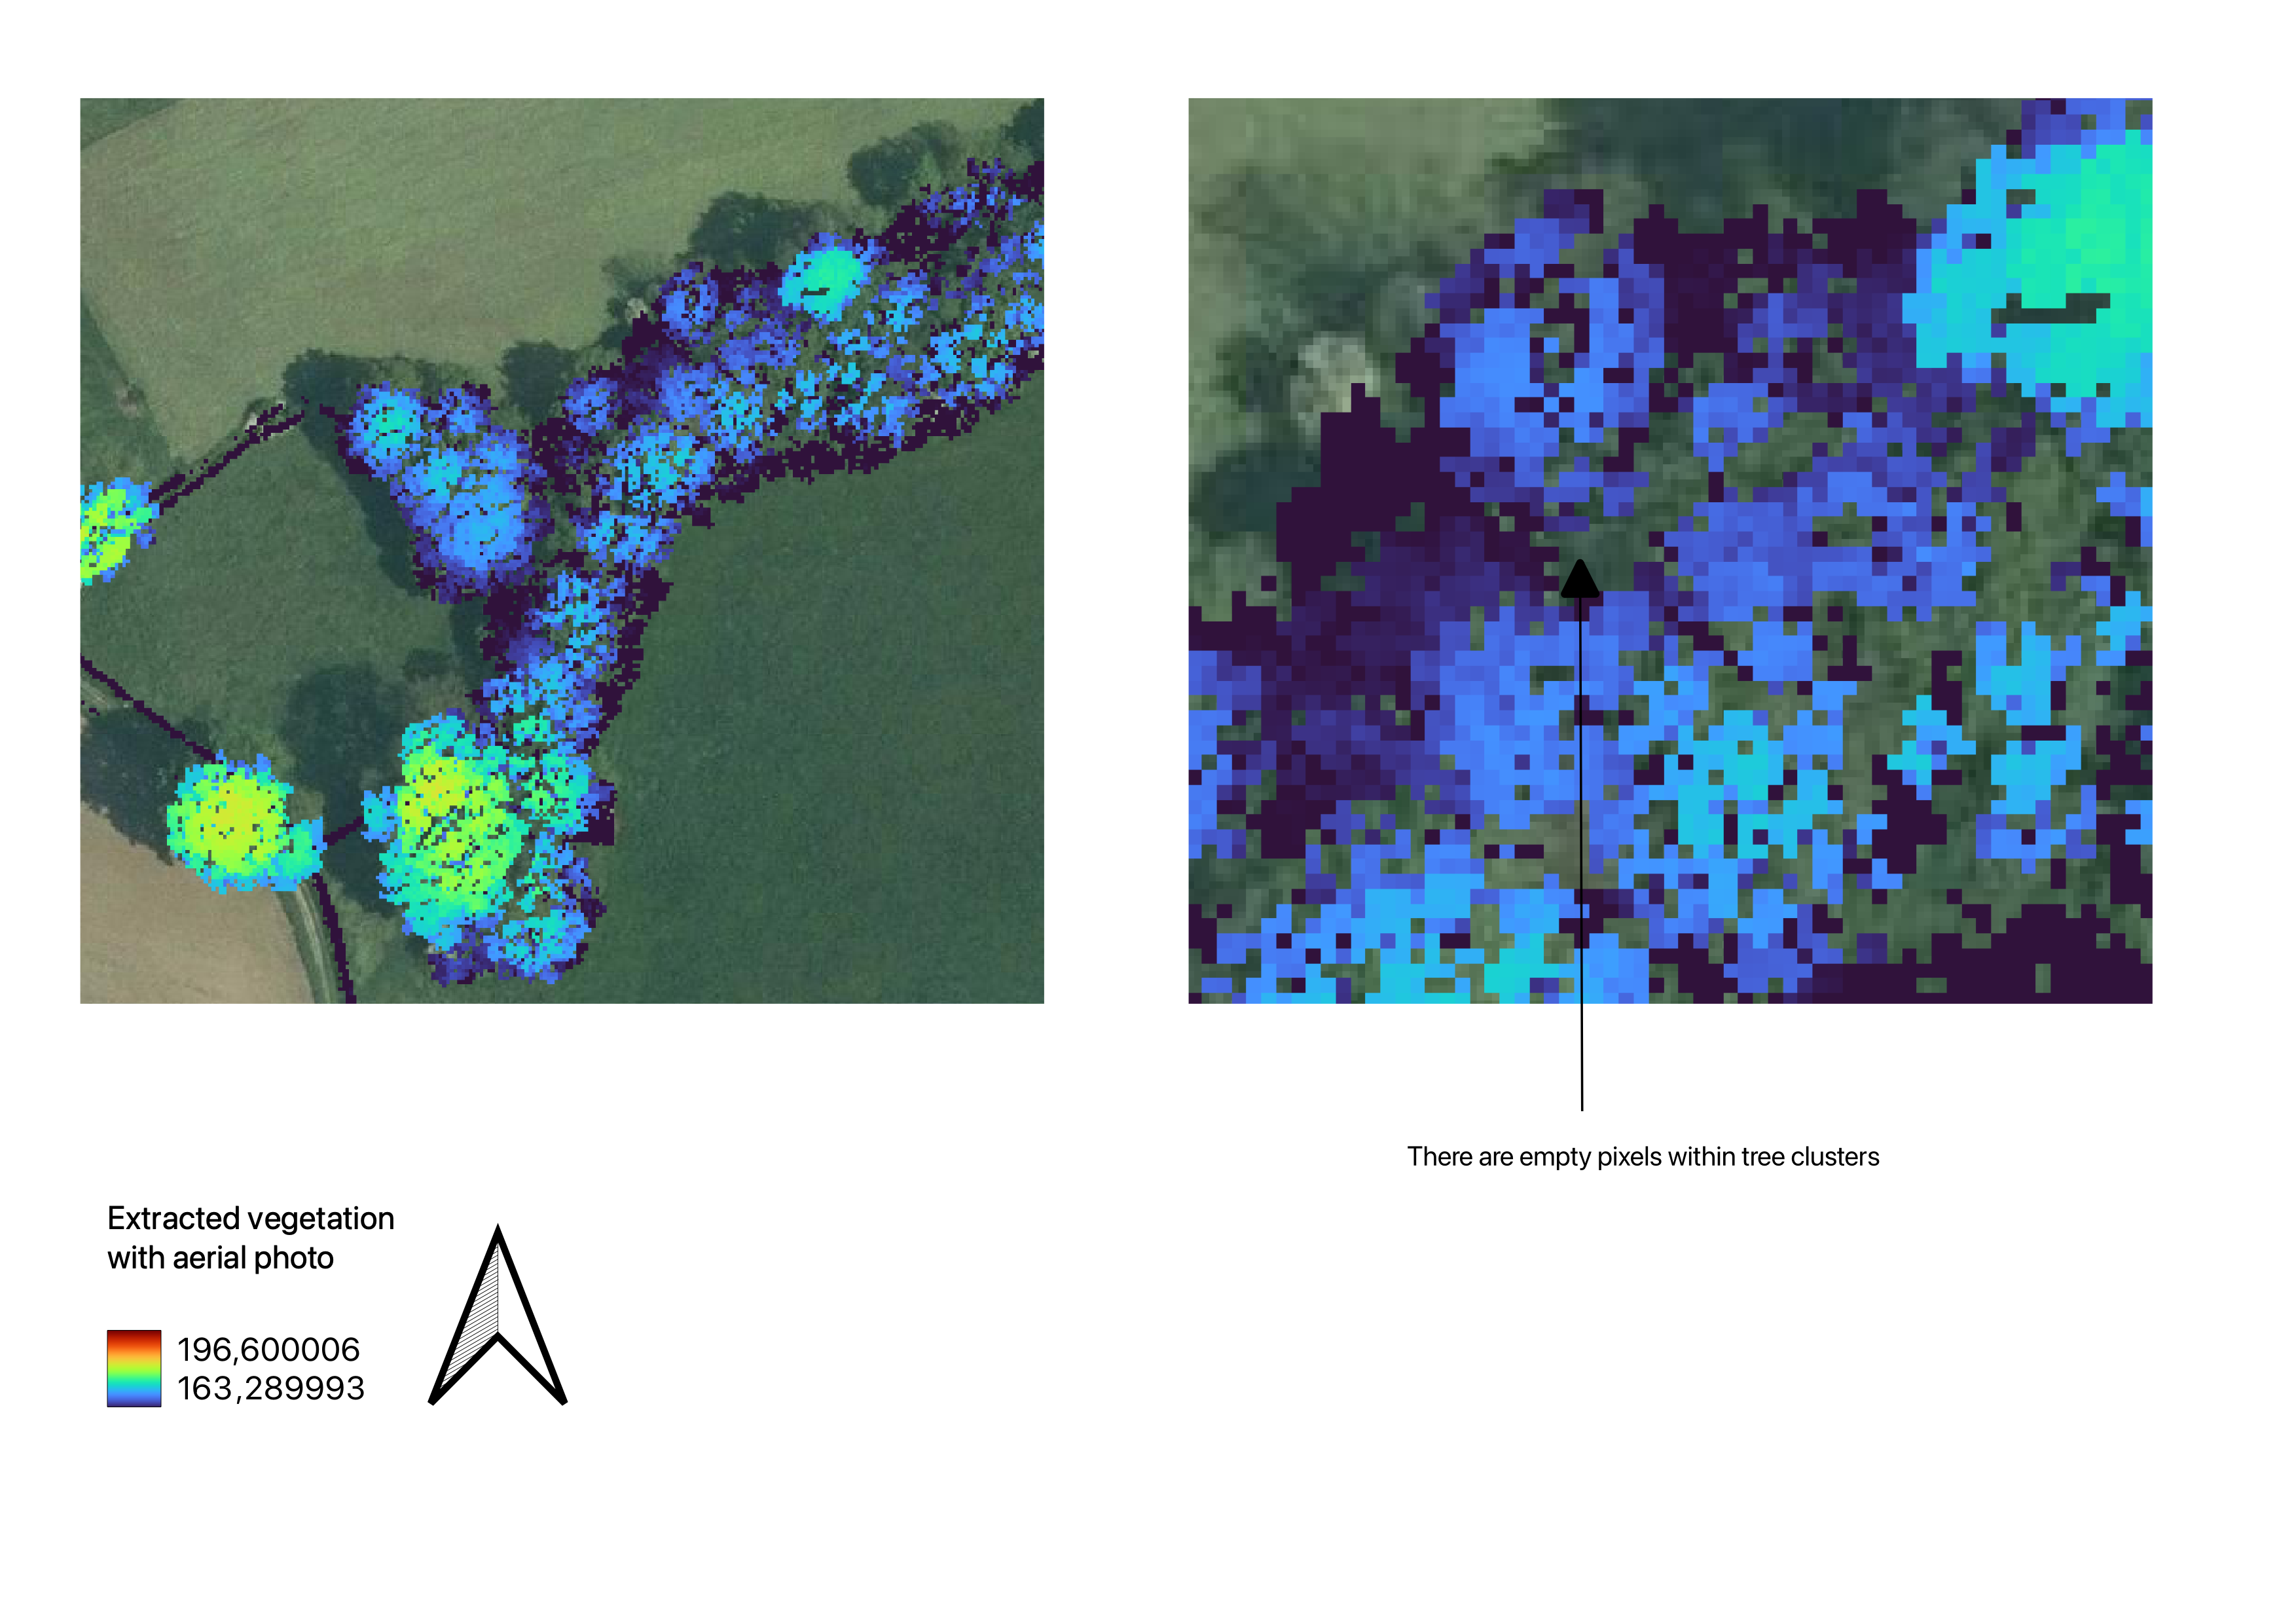
\includegraphics[width=0.7\linewidth]{Figures/numofreturnimprovment.png}
    \caption{Zoomed-in Result Using Number of Returns}
    \label{numofreturnsimprovement}
\end{figure}

\noindent To address this, we propose a strategy of filling in pixel values within the convex hull of each tree cluster. Once we have identified and assigned unique cluster IDs to trees during the vegetation extraction process, we can apply interpolation to fill in these empty cells located within the convex hulls of these tree clusters during rasterization. We anticipate that this approach will effectively resolve the issue of empty pixels within tree areas, ensuring a more continuous and accurate representation of the vegetation in our rasterized data.\\

\noindent \textbf{Intensity}\\
Overall, we decided to not go into the direction of implementing intensity into the main code. This was due to the fact that we were not able to find acceptable parameters that could fit different datasets. We found that the AHN4 dataset includes some inconsistencies in classifying vegetation from unidentified buildings. This tile we found while testing, showed in Figure~\ref{testc} on the right, depicted that even though there are many buildings on the from the aerial RGB photo (left Figure~\ref{testrgb}), they are not classified as buildings. This then changes the range of values when attempting to calculate statistical methods such as Z-Score to accurately extract vegetation only. The range of intensity changing affects extraction because there are now buildings that have intensities in the same range as vegetation. \\


\begin{figure}[H]
    \centering
    \subfloat[Test Tile]{%
        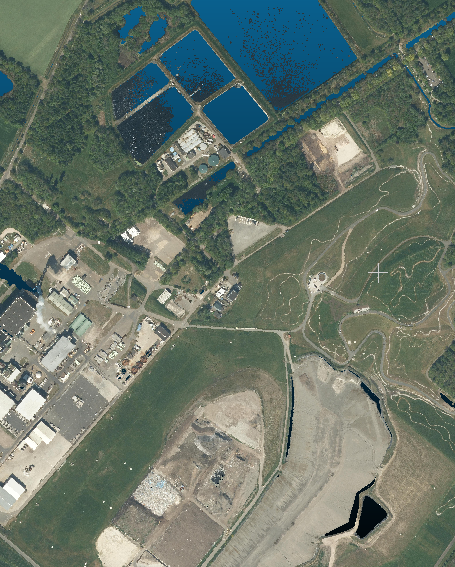
\includegraphics[width=0.3\linewidth]{Figures/testrgb.png}
        \label{testrgb}
    }
    \hspace{0.5cm}
    \subfloat[Test Tile Classification]{%
        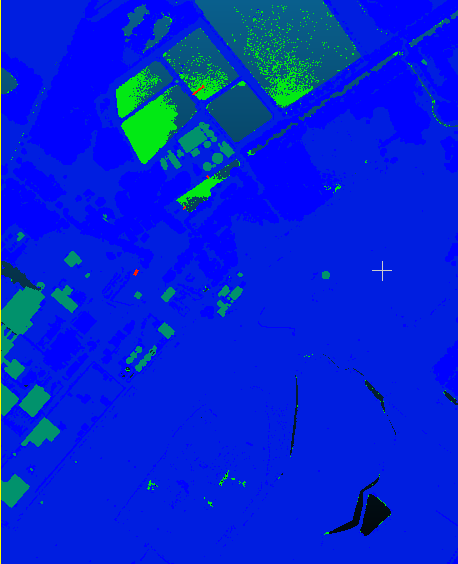
\includegraphics[width=0.3\linewidth]{Figures/testclass.png}
        \label{testc}
    }
    \caption{Classification (unclassified) Inconsistency}
    \label{fig:comparison}
\end{figure}


\subsection{Step 5: Canopy Height Model}
In the final phase of our research assignment, we successfully generated a Canopy Height Model (CHM) using data derived from previous steps. The process for creating the CHM was straightforward yet effective. We utilized the Digital Terrain Model (DTM) developed in Step 3 and the vegetation data extracted in Step 4. By subtracting the DTM values from the vegetation data, we were able to calculate the height of the vegetation canopy above the ground, thus creating the CHM. Figure~\ref{step5} shows this.\\

\begin{figure}[H]
    \centering
    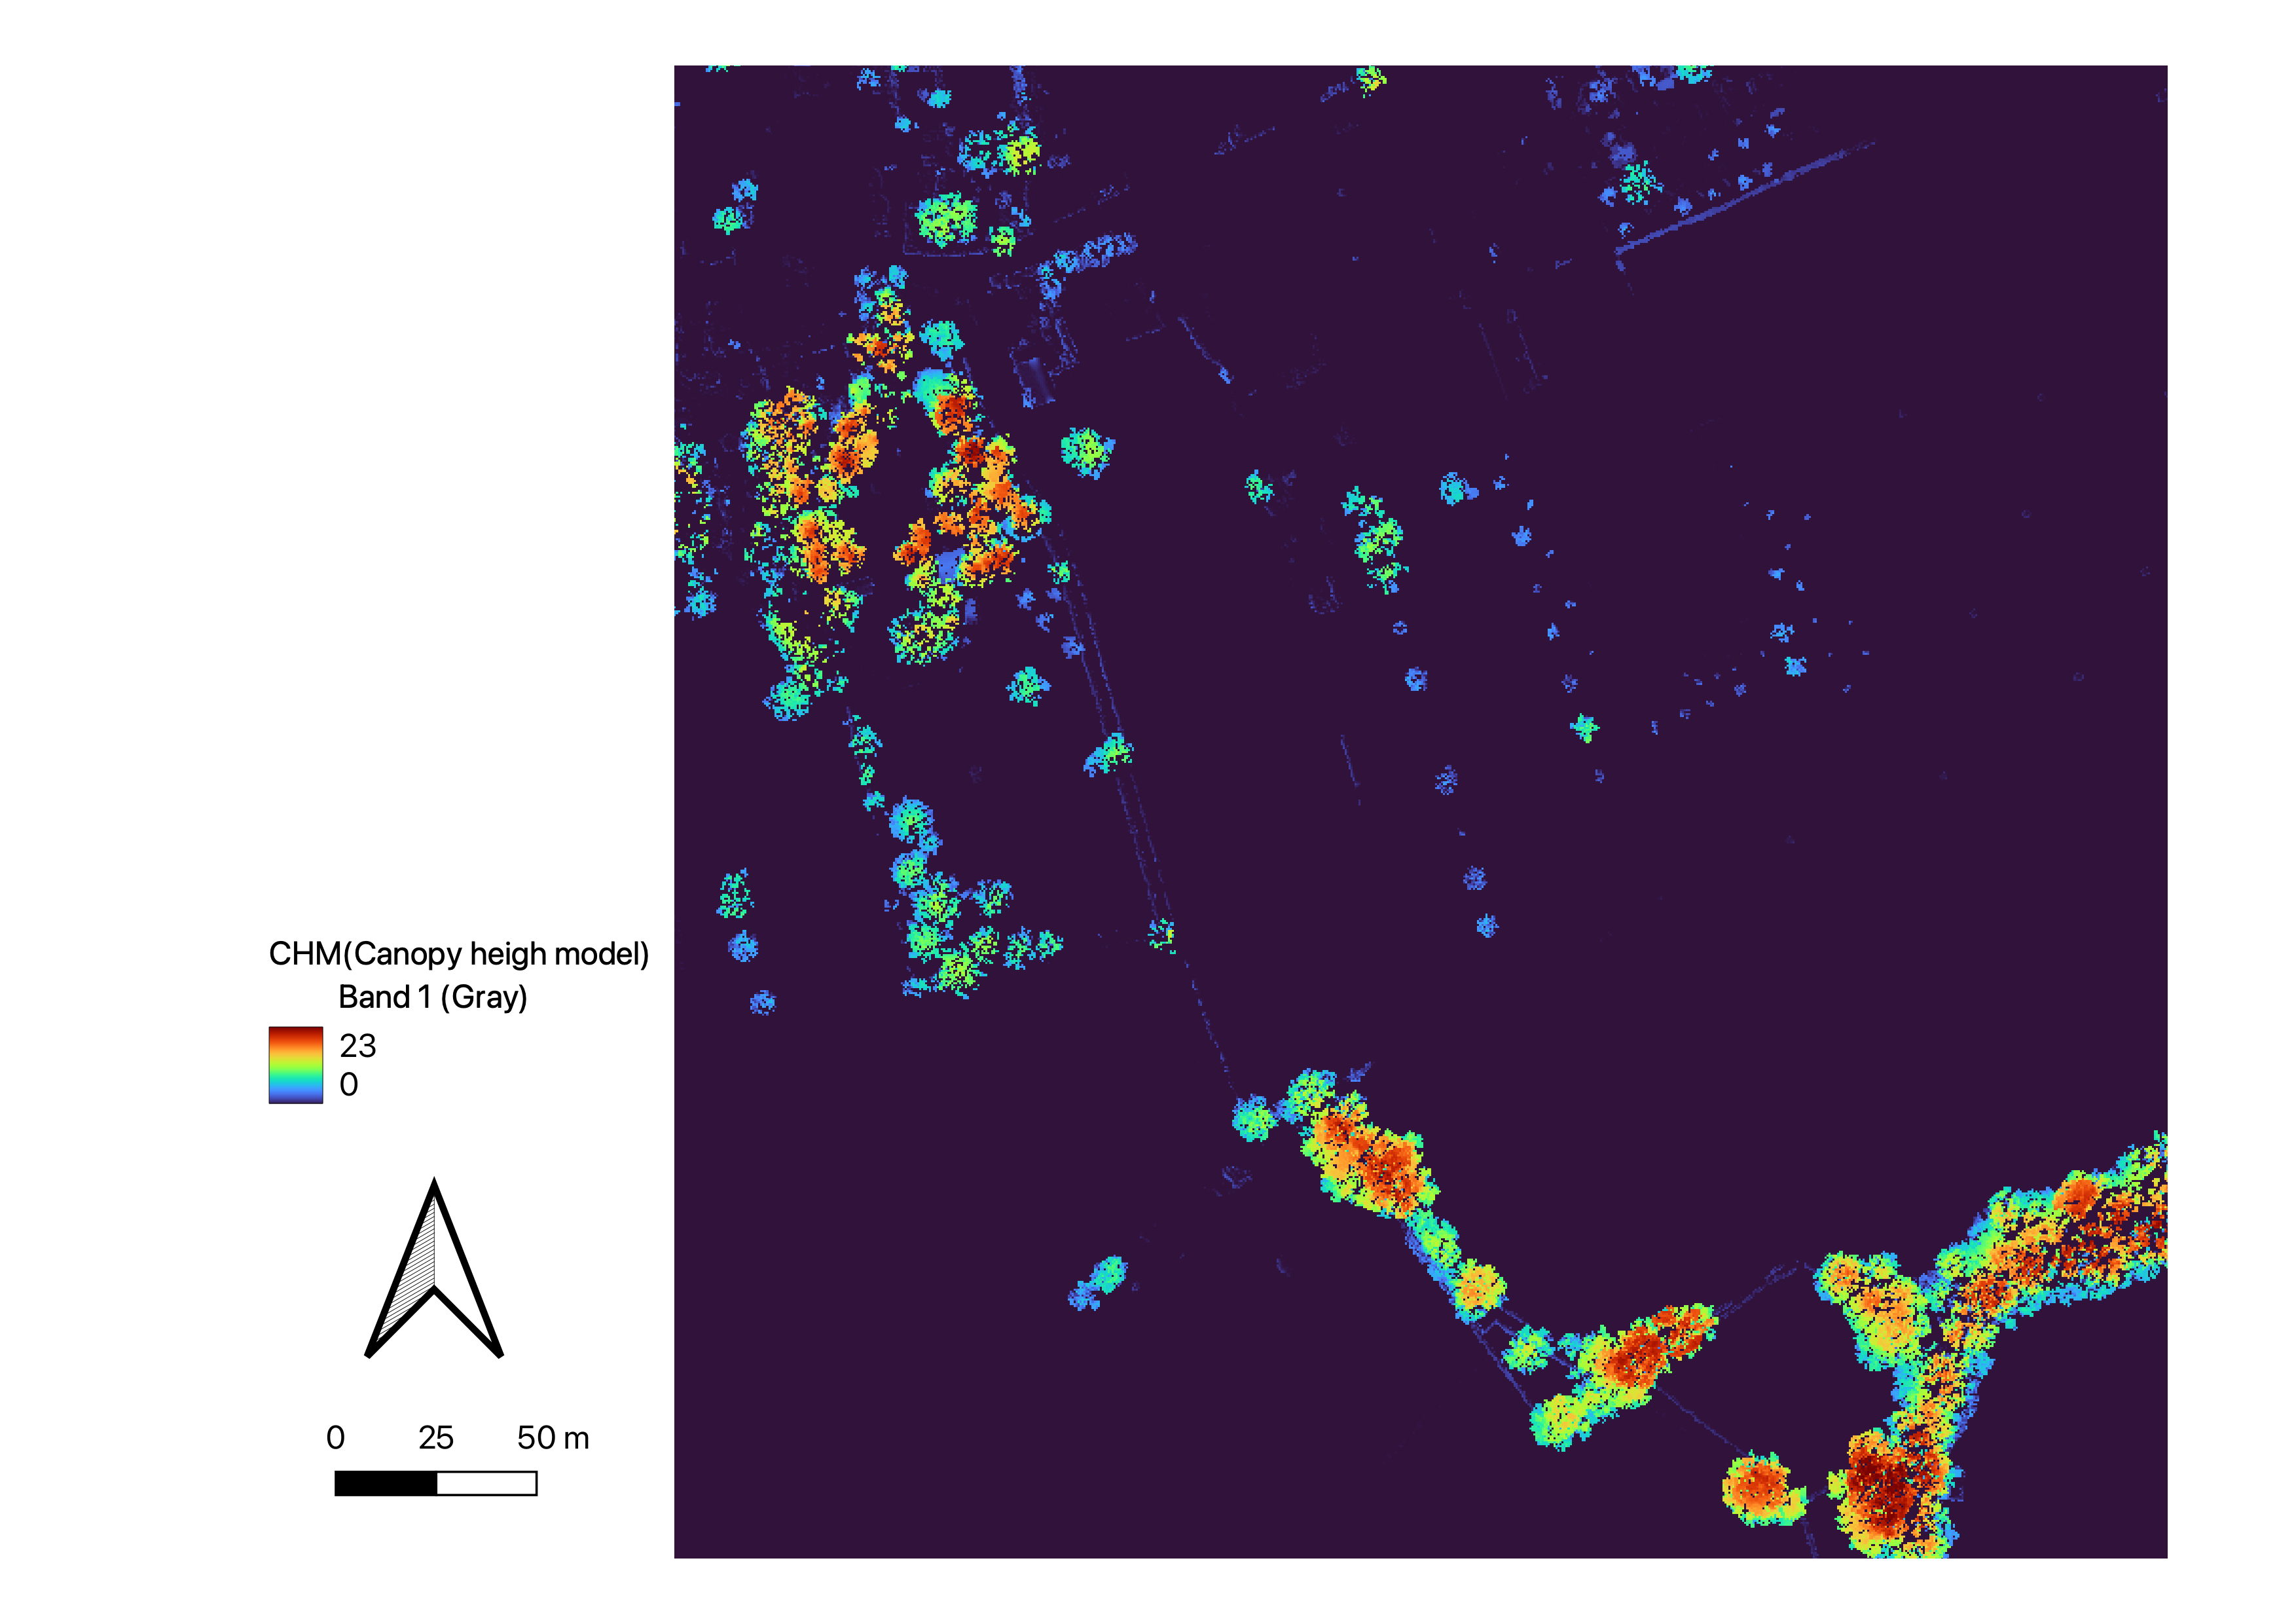
\includegraphics[width=0.7\linewidth]{Figures/step5.png}
    \caption{Canopy Height Model}
    \label{step5}
\end{figure}


\noindent The resultant CHM values range from 0 to approximately 23 meters, which aligns well with the expected tree heights in our study area and thus attests to the reasonableness of our model.\\

\noindent A comparative analysis between the vegetation height model from Step 4 and the CHM provided additional insights. Notably, while the top-left corner of the study area was characterized by many tall trees, the CHM revealed that even taller trees are present in the bottom-right corner. This observation underscores the value of the CHM in providing nuanced insights into the spatial distribution of tree heights across the area. The ability of the CHM to highlight these differences in canopy height is particularly useful, as it offers a more detailed understanding of the vertical structure of the vegetation, which is crucial for various ecological and environmental analyses.



\section{Conclusion}
The report delineates the steps taken to test the processing of point cloud data, mainly applying Ground Filtering algorithm to extract the ground points, and using number-of-returns and intensity from the point cloud metadata to extract vegetation from the unclassified set of AHN4 data. These were later used to make the final Canopy Height Model (CHM). While the source code can be found in \href{https://github.com/HideBa/geo1015-ass4-team-bbq}{GitHub}, the report mainly focused on the process of how we tackled certain points in implementing the algorithm.\\

\noindent For Step 3 (\ref{step3}), we used accuracy and F1 score to choose the optimal parameter for the Ground Filtering algorithm. The final chosen parameters were a distance threshold of 5 meters, a maximum angle of 30 degrees, and a cell size of 90 meters. The evaluation of our implementation was compared with the actual AHN4 data, which yielded an accuracy of around 95.55\% and F1 score of 0.97.\\

\noindent For Step 4 (\ref{step4}), after weighing the pros and cons of different approaches, we tried using two respective metadata for vegetation extraction: number of returns and intensity. The number of returns yielded a satisfactory result using DBSCAN. There is room for improvement, however, to fill in the missing pixels. This can be a future research subject, which uses a convex hull of each tree cluster to interpolate the missing values. Using intensity was attempted, but was not selected for the final method due to its inconsistency in different datasets. Final CHM was created using the result from Step 3 and the result using number of returns.\\ 

\noindent It was a very challenging and at the same time an interesting assignment. It provided us with a good insight on different metadata point cloud data has, and ways that we can process them to use for different purposes. 


\section{Work Distribution}
We had a number of collaborative discussions on the algorithm's functioning for a comprehensive understanding. Each team member individually tried to implement the algorithm. For step 4, we brainstormed the best method for implementation after individual research, which resulted in the 2 different methods as shown in the report. Hide's code worked successfully, which is the final result in GitHub. Shawn tried the intensity method for Step 4. For the report, Hide focused on elaborating Step 3 and the DBSCAN algorithm, Shawn concentrated on intensity-related aspects, and Hyeji took charge of the other sections and the overall layout. 
\clearpage


\bibliographystyle{apacite}
\bibliography{References/references}
\clearpage

\appendix
\section{Performance Challenges in Implementing Laplace Interpolation}
\noindent During the implementation of Laplace interpolation in our project, we encountered significant challenges related to the speed of execution. The interpolation process was taking an inordinately long time, prompting a need for a thorough investigation. To diagnose the cause of this poor performance, we utilized a line profiler to analyze the execution time of our code on a line-by-line basis.\\

\noindent The results of this profiling are illustrated below, which displays our interpolation code alongside the execution time for each line. A critical observation from this analysis is that a substantial amount of time is consumed when referencing points within startinpy's triangulation network. These specific lines of code were identified as the bottleneck of our program.\\

\begin{lstlisting}[language=Python, caption={Interpolation Code with Execution Time}, label={code1},basicstyle={\fontsize{5.5}{10}\selectfont\ttfamily}][H]
Line #      Hits         Time  Per Hit   % Time  Line Contents
==============================================================
    21                                               @profile
    22                                               def _laplace_interpolate(self, p):
    23                                                   """
    24                                                   Performs Laplace interpolation at a given point.
    25                                           
    26                                                   Args:
    27                                                       p (list): The coordinates of the point [x, y].
    28                                           
    29                                                   Returns:
    30                                                       float: The interpolated value at the given point.
    31                                                   """
    32                                           
    33       400        207.0      0.5      0.0          p = [p[0], p[1], 0.0]
    34       400       8282.0     20.7      0.0          p_index = self.dt.insert_one_pt(p[0], p[1], p[2])
    35       400        452.0      1.1      0.0          if self.dt.is_vertex_convex_hull(p_index):  # impossible to interpolate
    36                                                       self.dt.remove(p_index)
    37                                                       return np.nan
    38       400      30191.0     75.5      0.0          triangles = self.dt.incident_triangles_to_vertex(p_index)
    39                                           
    40       400         80.0      0.2      0.0          weight_z_pairs = []
    41      2988       6962.0      2.3      0.0          for i, tri in enumerate(triangles):
    42      2588       7899.0      3.1      0.0              p0_i, p1_i, p2_i = tri
    43      2588       5061.0      2.0      0.0              p0, p1, p2 = (
    44      2588   18000104.0   6955.2     11.0                  tuple(self.dt.points[p0_i]),
    45      2588   18067023.0   6981.1     11.1                  tuple(self.dt.points[p1_i]),
    46      2588   18093927.0   6991.5     11.1                  tuple(self.dt.points[p2_i]),
    47                                                       )
    48      2588       7592.0      2.9      0.0              next_tri = triangles[(i + 1) % len(triangles)]
    49      2588       3085.0      1.2      0.0              p3_i, p4_i, p5_i = next_tri
    50      2588       5338.0      2.1      0.0              p3, p4, p5 = (
    51      2588   18110375.0   6997.8     11.1                  tuple(self.dt.points[p3_i]),
    52      2588   18090358.0   6990.1     11.1                  tuple(self.dt.points[p4_i]),
    53      2588   18081831.0   6986.8     11.1                  tuple(self.dt.points[p5_i]),
    54                                                       )
    55                                           
    56      5176       4891.0      0.9      0.0              common_points_indices = list(
    57      2588      17620.0      6.8      0.0                  set([p0_i, p1_i, p2_i]).intersection(set([p3_i, p4_i, p5_i]))
    58                                                       )
    59      2588      25816.0     10.0      0.0              cc1 = self._circimcircle_center(p0, p1, p2)
    60      2588       7701.0      3.0      0.0              cc2 = self._circimcircle_center(p3, p4, p5)
    61      2588       1084.0      0.4      0.0              if cc1 is None or cc2 is None:
    62                                                           continue
    63      2588       6941.0      2.7      0.0              voronoi_edge_length = math.dist(cc1, cc2)
    64      5176     513582.0     99.2      0.3              edge = math.dist(
    65      2588   17827431.0   6888.5     10.9                  self.dt.points[common_points_indices[0]],
    66      2588   18173467.0   7022.2     11.1                  self.dt.points[common_points_indices[1]],
    67                                                       )
    68      2588       2294.0      0.9      0.0              weight = voronoi_edge_length / edge
    69      2588      40810.0     15.8      0.0              common_points_indices.remove(p_index)
    70      2588   18023326.0   6964.2     11.0              z = self.dt.points[common_points_indices[0]][2]
    71      2588       9905.0      3.8      0.0              weight_z_pairs.append([weight, z])
    72       800       3723.0      4.7      0.0          interpolated_value = sum([w * z for w, z in weight_z_pairs]) / sum(
    73       400        513.0      1.3      0.0              [w for w, _ in weight_z_pairs]
    74                                                   )
    75                                           
    76       400       2939.0      7.3      0.0          self.dt.remove(p_index)
    77       400         69.0      0.2      0.0          return interpolated_value
\end{lstlisting}


\noindent This led us to question why startinpy’s interpolation method exhibited significantly faster performance compared to our implementation. The bottleneck, interestingly, occurs at the same point of referencing triangulation points in both implementations. Upon examining startinpy’s implementation, we noticed that it employs a \textit{link} structure to efficiently access linked vertices of a given vertex. However, the Python interface of startin returns all points as a NumPy array. We hypothesize that the conversion from startinpy’s internal array structure to a Python-compatible NumPy array format, particularly in scenarios involving a large number of vertices, is a time-consuming process. This conversion step is likely contributing to the slower performance of our implementation compared to the native execution in startinpy.\\



\begin{lstlisting}[language=Python, caption={\protect\href{https://github.com/hugoledoux/startinpy/blob/d99e96c7818b9003801db48085b46e54c0db03a0/src/lib.rs#L73C1-L76C6}{Code to Convert startin Data Structure to Python Data Structure}}, label={code2}][H]
   fn points<'py>(&self, py: Python<'py>) -> PyResult<&'py PyArray<f64, numpy::Ix2>> {
        let vs = self.t.all_vertices();
        Ok(PyArray::from_vec2(py, &vs).unwrap())
    }
    
\end{lstlisting}

\noindent Understanding this bottleneck has provided us with valuable insights into potential areas for optimization in our interpolation code. It suggests that modifying our approach to handle triangulation point references more efficiently, or minimizing the need for conversion to NumPy arrays, could significantly improve the performance of our Laplace interpolation implementation.\\


\end{document}







